% AgenticTO Guidebook. Build: see README.md in this folder (latexmk -pdf guidebook.tex).
\documentclass[11pt,a4paper,twoside,openany]{book}
\usepackage{agentto-guide}
% Generated by docs/guidebook/gen_tables.py from the code. Do not edit by hand.
\newcommand\LadderMax{$8\times10^{7}$}
\newcommand\LadderMin{5000}
\newcommand\MgSwitch{$6\times10^{7}$}
\newcommand\MgRetry{$6.6\times10^{7}$}
\newcommand\MaxOuter{300}
\newcommand\MovingPPM{100}
\newcommand\SketchCells{40}
\newcommand\SpillEvery{10}
\newcommand\SolveTimeout{900}
\newcommand\VolTol{0.001}
\newcommand\MgIRBytes{146}
\newcommand\MgSixtyFourBytes{366}
\newcommand\CheckDelay{300}
\newcommand\RungNames{sketch, preview, refine, release}
\newcommand\NTools{27}
\newcommand\NToolsSpec{16}
\newcommand\NToolsClarify{17}
\newcommand\NToolsFull{27}


\graphicspath{{../user_guide/img/}{figures/}}
\makeindex[intoc,columns=2,title=Index,options={-s index.ist}]
\indexsetup{othercode={\setlength{\parskip}{0pt plus 0.3pt}\small}}

\hypersetup{pdftitle={AgenticTO Guidebook},
  pdfauthor={Shaoliang Yang and Jun Wang},
  pdfsubject={Agent-assisted, certified 3D topology optimization on one GPU},
  pdfkeywords={topology optimization, language agents, design specification, certificate, MCP}}

\newcommand\rref[1]{\hyperref[rule:#1]{\textsf{\bfseries #1}}}
\newcommand\repourl{https://github.com/nbbllxx0/From-brief-design-to-verified-release}
\newcommand\papertitle{From topology-optimization brief to solver-checked release: separating intent,
admissibility and acceptance knowledge for language agents}

\begin{document}
\frontmatter
% Title page and colophon
\begin{titlepage}
\thispagestyle{empty}
\begin{tikzpicture}[remember picture,overlay]
  \fill[guigrey] (current page.north west) rectangle ([yshift=-104mm]current page.north east);
  \fill[okgreen] ([yshift=-104mm]current page.north west) rectangle ([xshift=70mm,yshift=-106.5mm]current page.north west);
  \fill[okamber] ([xshift=70mm,yshift=-104mm]current page.north west) rectangle ([xshift=140mm,yshift=-106.5mm]current page.north west);
  \fill[okblue]  ([xshift=140mm,yshift=-104mm]current page.north west) rectangle ([yshift=-106.5mm]current page.north east);
  \node[anchor=north west,text=white,font=\sffamily\bfseries\fontsize{13}{15}\selectfont,align=left]
    at ([xshift=30mm,yshift=-30mm]current page.north west) {GUIDEBOOK\enspace{\mdseries\color{white!70!guigrey}$\cdot$\enspace Version \AgenticVersion}};
  \node[anchor=north west,text=white,font=\sffamily\bfseries\fontsize{52}{56}\selectfont]
    at ([xshift=29mm,yshift=-40mm]current page.north west) {AgenticTO};
  \node[anchor=north west,text=white!88!guigrey,font=\sffamily\fontsize{15}{20}\selectfont,align=left,text width=150mm]
    at ([xshift=30mm,yshift=-66mm]current page.north west)
    {Agent-assisted, certified 3D topology optimization on one GPU:\\ the workspace, the tool contract and the release record};
  \node[anchor=north,inner sep=0] at ([yshift=-122mm]current page.north)
    {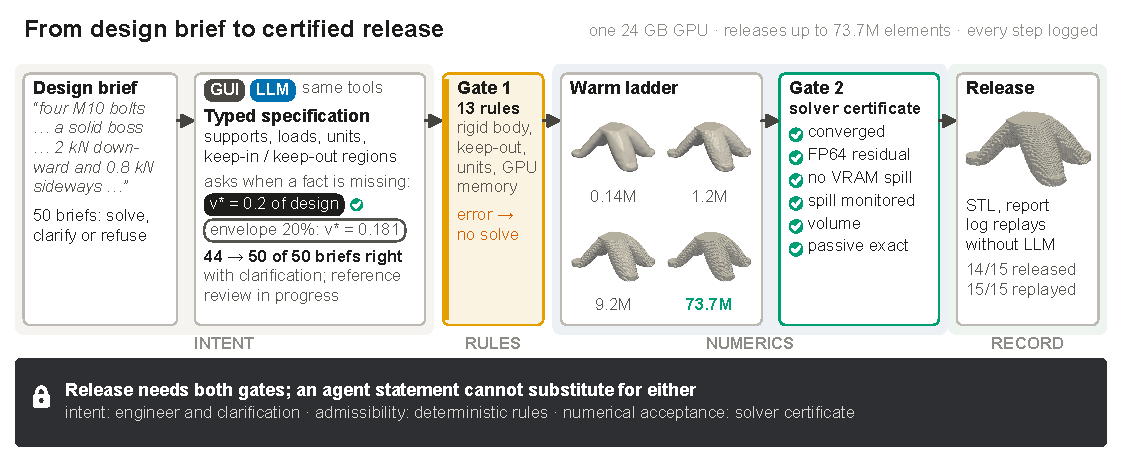
\includegraphics[width=160mm]{graphical_abstract_art.pdf}};
  \node[anchor=north west,font=\sffamily,align=left,text width=150mm] at ([xshift=30mm,yshift=-200mm]current page.north west)
    {{\fontsize{14}{18}\selectfont\bfseries Shaoliang Yang \quad Jun Wang}\\[2mm]
     {\color{muted}Department of Mechanical Engineering, Santa Clara University}\\[9mm]
     {\small\color{muted}Companion to the paper}\\[1mm]
     {\small\itshape\rmfamily \papertitle}};
  \node[anchor=south west,font=\sffamily\small\color{muted},align=left,text width=150mm]
    at ([xshift=30mm,yshift=22mm]current page.south west)
    {October 2026\hfill Software version \AgenticVersion, spec schema \texttt{agentto.spec/v0}};
\end{tikzpicture}
\end{titlepage}

% ---- colophon ----
\thispagestyle{empty}
\vspace*{\fill}
{\small\sffamily
\textbf{AgenticTO Guidebook}\\
Version \AgenticVersion, October 2026. Describes AgenticTO \AgenticVersion\ (Python package \code{agentto}) and the
specification schema \code{agentto.spec/v0}.

\medskip
\textbf{Authors.} Shaoliang Yang and Jun Wang, Department of Mechanical Engineering, Santa Clara University,
500 El Camino Real, Santa Clara, CA 95053, USA. Correspondence: Jun Wang, \href{mailto:jwang22@scu.edu}{jwang22@scu.edu}.

\medskip
\textbf{Software.} The application code, the 50-brief task suite with its adjudicated reference readings, the saved
agent outputs and tool logs, the numerical result records, the generators of the tables and data figures, and the
\code{voxfem} solver that AgenticTO runs on (BSD 3-Clause; Chapter~\ref{ch:install}) are available at \url{\repourl}.

\medskip
\textbf{How this book is made.} The reference tables for the specification schema, the rules, the tools, the certificate,
the schedules, the command-line flags, the HTTP endpoints, the keyboard map and the script catalogue are generated from
the source code by \code{docs/guidebook/gen\_tables.py}, so they match the code they describe. Every screenshot comes from a
real session recorded by \code{scripts/guide\_shots.py}, which drives the workspace with real clicks and keystrokes.
Numbers about performance and accuracy are taken from the paper or from the result files it cites, never measured
again for this book; each such number is marked with its claim identifier from \code{results/claims\_ledger.md}, for
example \claim{C3.1}.

\medskip
\textbf{Scope.} AgenticTO is research software. A certificate in this book means a set of numerical acceptance checks
on a stated computation. It is not a structural safety assessment, and a released design needs further engineering
analysis before anything is built from it.

\medskip
\textbf{Typography.} Set in XCharter, Helvetica and Inconsolata. Colours follow the paper's figures: green for a passing
check, vermillion for a failure, blue for the agent, amber for the rule gate, dark grey for the workspace.
}
\clearpage

\chapter*{Preface}
\addcontentsline{toc}{chapter}{Preface}
\markboth{Preface}{Preface}

A topology optimization can converge and still solve the wrong problem. A support may restrain a direction the
engineer meant to leave free, a load may sit on the wrong face, a pad may be retained that nobody asked for. Neither the
solver's residual nor a language agent's confident summary reveals such errors. AgenticTO is built around that
observation. It keeps the design intent in one typed specification, checks it with deterministic rules before anything
is solved, and lets only the solver issue the certificate that marks a result as released. A language agent can help
at every step, but it works through the same logged tools as the engineer and cannot write a certificate.

This guidebook explains how to install the software, build and solve designs in its graphical workspace, work with the
built-in assistant, connect other agents through the Model Context Protocol, read the provenance log, and reproduce the
results of the companion paper.

\paragraph{Who this book is for.} Two groups of readers. Journal reviewers who want to know what the software actually
does, which check is responsible for which guarantee, and how each number in the paper can be traced to a file and a
script: Chapters~\ref{ch:overview}, \ref{ch:ladder}, \ref{ch:reproduce} and \ref{ch:limits} are written for you.
Engineers who download the public release and want to use it: start with Chapters~\ref{ch:install} and
\ref{ch:quickstart}, then read the chapters on the workspace, the specification and the rules.

\paragraph{How to read it.} Chapter~\ref{ch:overview} gives the concepts in a few pages. Chapter~\ref{ch:quickstart}
takes you from a fresh start to a certified, exported design in about ten minutes. The remaining chapters can be read in
any order. The appendices are reference material: every field of the specification, every tool with its arguments,
every certificate field, the keyboard map, every script, and a glossary. A one-page quick reference precedes the
index.

\paragraph{Conventions.}
\begin{itemize}
  \item Interface labels are set in bold sans serif: \gui{Optimize release}. Keys look like \keycap{S} or
        \keycap{Ctrl}+\keycap{K}.
  \item File names, commands, tool names and JSON fields are set in monospace: \code{scripts/serve.py},
        \tool{validate_spec}, \code{volume\_fraction}. Tool names link to their reference entry in
        Appendix~\ref{app:tools}; rule codes such as \rref{R003} link to Chapter~\ref{ch:rules}.
  \item Commands are shown for a POSIX shell. On Windows, the same commands work in PowerShell except where a box says
        otherwise.
  \item A grey bracket such as \claim{C2.3} names the claim in \code{results/claims\_ledger.md} that backs a number.
\end{itemize}

\begin{tipbox}[Four kinds of boxes]
Green boxes like this one give practical tips. Blue boxes add background. Vermillion boxes warn about something that
can cost you a result or mislead you. Amber boxes quote evidence from the paper, with its denominator.
\end{tipbox}

\paragraph{Acknowledgement of tools.} The software was developed with the help of OpenAI Codex and Claude-based
coding tools, as stated in the paper's declaration. This guidebook was drafted with AI assistance from the source code, the
existing user guide and the paper; its reference tables are generated from the code.

{\hypersetup{linkcolor=ink}\tableofcontents}

\mainmatter
\chapter{What AgenticTO is}\label{ch:overview}
\chapterintro{AgenticTO turns a written design brief into a certified 3D topology-optimized part. This chapter explains
the three independent checks the system is built around, the five objects you will meet everywhere, who may do what,
and how the parts of the software fit together.}

AgenticTO minimizes the compliance of a structure (maximizes its stiffness) under a material budget, on a regular voxel
grid, with the density-based SIMP method and a GPU multigrid solver. You describe the problem: a box of space, its
supports and loads, regions that must stay solid or empty, a material and a volume fraction. AgenticTO solves it on a
ladder of ever finer grids, up to several times $10^7$ elements on one 24~GB graphics card, and exports the result as a
closed STL surface with a report.

What sets the system apart is not the solver, which comes from companion work, but the way it separates the questions
that have to be answered before a result can be trusted. A design can fail in three different ways, and each needs its
own check.

\section{Three checks, three kinds of knowledge}\label{sec:threechecks}
\index{three checks}

\begin{figure}[t]
\centering
\begin{tikzpicture}[font=\sffamily\footnotesize,
  box/.style={draw=#1,line width=0.8pt,fill=#1!8,rounded corners=2pt,align=center,minimum height=13mm,
    text width=23.5mm,inner sep=2pt},
  arr/.style={-{Stealth[length=2.2mm]},line width=0.7pt,color=guigrey}]
  \node[box=guigrey] (brief) {\textbf{Brief}\\written text};
  \node[box=okblue,right=4.5mm of brief] (spec) {\textbf{Specification}\\\texttt{agentto.spec/v0}};
  \node[box=okamber,right=4.5mm of spec] (rules) {\textbf{Rule gate}\\R001--R013};
  \node[box=guigrey,right=4.5mm of rules] (ladder) {\textbf{Ladder}\\sketch $\rightarrow$ release};
  \node[box=okgreen,right=4.5mm of ladder] (cert) {\textbf{Certificate}\\six predicates};
  \draw[arr] (brief) -- (spec);
  \draw[arr] (spec) -- (rules);
  \draw[arr] (rules) -- (ladder);
  \draw[arr] (ladder) -- (cert);
  \node[below=2.5mm of spec,text width=34mm,align=center,color=okblue] (q1)
    {\textbf{Intent}\\Is this the problem the engineer meant?\\[1pt]{\color{muted}engineer, clarification}};
  \node[below=2.5mm of rules,text width=30mm,align=center,color=okamber!80!black] (q2)
    {\textbf{Formulation}\\Is the problem admissible?\\[1pt]{\color{muted}deterministic rules}};
  \node[below=2.5mm of cert,text width=32mm,align=center,color=okgreen!75!black] (q3)
    {\textbf{Numerics}\\Did this computation meet its requirements?\\[1pt]{\color{muted}solver-issued record}};
  \draw[decorate,decoration={brace,amplitude=4pt,mirror},color=rulegrey] ([yshift=-1mm]brief.south west) -- ([yshift=-1mm]spec.south east);
\end{tikzpicture}
\caption{The path from a brief to a released design, and the question each check answers. A design is released only
when all three are settled: the engineer (helped by clarification) settles intent, the rules settle admissibility,
and the solver's certificate settles numerical acceptance.}
\label{fig:threechecks}
\end{figure}

Figure~\ref{fig:threechecks} shows the path from a brief to a released design.

\begin{description}
  \item[Intent.] Does the specification say what the engineer meant? Only the engineer can answer this, so AgenticTO
  makes the specification readable and editable, shows every region in the viewport, and lets the assistant ask a
  question when a brief leaves a design-changing fact open (Chapter~\ref{ch:assistant}).
  \item[Formulation.] Is the stated problem admissible at all? Thirteen deterministic rules check it within
  milliseconds of every edit: free rigid-body motion, regions that select nothing, a load inside a keep-out region,
  overlapping keep-in and keep-out regions, a grid too large for the GPU, and more (Chapter~\ref{ch:rules}). Any error
  blocks solving.
  \item[Numerics.] Did the computation meet its own requirements? The solver issues a certificate with six predicates:
  convergence, an accepted FP64 state solve, no GPU memory spill, active spill monitoring, the volume within
  $10^{-3}$, and exact keep-in and keep-out regions (Chapter~\ref{ch:ladder}). Only a certified result on the release
  rung is a released design.
\end{description}

The three checks are not redundant. Each catches failures the others pass, and the paper shows this with
experiments.

\begin{evidencebox}[Each check catches what the others miss]
\begin{itemize}[leftmargin=1.1em]
  \item \textbf{Intent errors pass the rules.} With grounding tools but without questions, the primary agent returned
  6 wrong specifications on 50 briefs, and all 6 passed every rule. With clarification it returned none
  \claim{C2.3, C4.2}.
  \item \textbf{A rule violation can pass the certificate.} With the rule gate switched off, a brief whose load sits
  inside its own keep-out region converged and received a passing numerical certificate, at about $3.8\times10^{8}$
  times the compliance of the corrected problem. Rule \rref{R008} stops it before any solve \claim{C4.4}.
  \item \textbf{The certificate holds back failed computations.} Of 54 recorded release attempts, 52 were certified;
  the census also contains 11 solves that ended without converging, which a system without the gate would have shown as
  designs \claim{C4.3}.
\end{itemize}
\end{evidencebox}

\section{The five objects}\label{sec:fiveobjects}
Five objects run through the whole system. Every chapter of this book is about one or more of them.

\begin{description}
  \item[The specification.]\index{specification} One typed, versioned JSON document (\code{agentto.spec/v0}) holds the
  design intent: units, domain, material, volume fraction, supports, loads, keep-in and keep-out regions, base mesh
  and an optional minimum feature size. The workspace, the assistant, external agents and scripts all edit this same
  document through the same tools. It is geometric, not discrete: a face stays a face when the mesh changes
  (Chapter~\ref{ch:spec}).
  \item[The rules.]\index{rules} Thirteen checks with stable codes R001--R013 run on every change. Errors block
  solving; warnings and notes stay visible with a suggested fix (Chapter~\ref{ch:rules}).
  \item[The ladder.]\index{resolution ladder} Each problem is solved on up to four rungs (sketch, preview, refine,
  release). Each rung has twice as many elements along every edge as the one below, so eight times as many in total, and
  starts from the design of the rung below (Chapter~\ref{ch:ladder}).
  \item[The certificate.]\index{certificate} Every finished solve carries a certificate created by the solver. No tool
  can write one. Only a certified result on the release rung is a finished design.
  \item[The log.]\index{session log} Every edit, agent step, answer and solve is written to \code{session.jsonl} with
  the actor who made it (user, agent, system or script) and the hash of the specification after it. A session can be
  replayed without any language model, and the solves reproduce bit for bit (Chapter~\ref{ch:provenance}).
\end{description}

\section{Who may do what}\label{sec:authority}
\index{authority}
AgenticTO makes authority explicit. Table~\ref{tab:authority} lists what each participant can do. The agent can
propose, edit, ask and solve, but the certificate comes only from the solver, and the export of a released design
requires a certified release-rung result.

\begin{table}[t]
\caption{Who may do what. ``Instruction'' marks a limit stated in the assistant's instructions rather than enforced by
the tool profile.}\label{tab:authority}
\newcolumntype{C}[1]{>{\centering\arraybackslash}p{#1}}
\begin{fixtable}{@{}>{\raggedright\arraybackslash}p{0.2\linewidth}C{0.09\linewidth}C{0.07\linewidth}%
C{0.09\linewidth}C{0.1\linewidth}C{0.1\linewidth}>{\raggedright\arraybackslash}X@{}}
 & Edit spec & Ask user & Solve sketch, preview & Solve refine, release & Write certificate & Notes \\ \midrule
Engineer in the workspace & \yes & -- & \yes & \yes & \no & starts every release in the GUI \\
Assistant, Propose & private copy & \yes & \no & \no & \no & changes come back as cards to accept \\
Assistant, Act & \yes & \yes & \yes & instruction: no & \no & a whole run can be undone in one step \\
External agent, \code{full} profile & \yes & \yes & \yes & \yes & \no & every call tagged \code{agent} in the log \\
Solver & \no & \no & -- & -- & \yes & from solver evidence only \\
\end{fixtable}
\end{table}

\begin{notebox}[A certificate is not a safety assessment]
The certificate states that a specific computation met specific numerical requirements on a stated grid. It does not
prove a global optimum, and it says nothing about stress, buckling, fatigue, manufacturability or the behaviour of
the exported surface as a physical part. Treat a released design as the input to further engineering analysis.
\end{notebox}

\section{How the software fits together}\label{sec:architecture}
\index{architecture}

\begin{figure}[t]
\centering
\begin{tikzpicture}[font=\sffamily\footnotesize,
  layer/.style={draw=#1,line width=0.8pt,fill=#1!7,rounded corners=2pt,align=left,inner sep=3pt,text width=38mm},
  arr/.style={{Stealth[length=2mm]}-{Stealth[length=2mm]},line width=0.6pt,color=guigrey},
  lab/.style={font=\sffamily\scriptsize,color=muted,fill=white,inner sep=1pt}]
  \node[layer=guigrey] (web) {\textbf{Web workspace}\\React + three.js, port 5173\\viewport, inspector, ladder, cards};
  \node[layer=guigrey,right=11mm of web] (api) {\textbf{Backend}\quad\code{scripts/serve.py}\\FastAPI, 127.0.0.1:8765\\one \code{Session}, \code{session.jsonl}};
  \node[layer=guigrey,right=11mm of api] (gpu) {\textbf{GPU worker}\\separate process, owns CUDA\\\code{SessionSIMP} on \code{voxfem}};
  \node[layer=okblue,below=12mm of web] (codex) {\textbf{Built-in assistant}\\Codex CLI (subscription)\\one session per message};
  \node[layer=okblue,below=12mm of api] (mcp) {\textbf{MCP server}\\\code{agentto.mcp\_server}\\stand-alone or \code{--attach}};
  \node[layer=okblue,below=12mm of gpu] (ext) {\textbf{External agents}\\Claude Code, Codex, any MCP client};
  \draw[arr] (web) -- node[lab,above]{WebSocket} (api);
  \draw[arr] (api) -- node[lab,above]{job queue} (gpu);
  \draw[arr] (codex) -- node[lab,above]{stdio} (mcp);
  \draw[arr] (ext) -- node[lab,above]{stdio} (mcp);
  \draw[arr] (mcp) -- node[lab,right]{HTTP \code{/api/tools}} (api);
  \draw[arr] (web) -- node[lab,right]{chat} (codex);
\end{tikzpicture}
\caption{Processes and connections. All edits, whether from the workspace, the assistant or an external agent, become
calls on the one \code{Session} in the backend and land in the same log. Solves run one at a time on the GPU worker.}
\label{fig:architecture}
\end{figure}

Figure~\ref{fig:architecture} shows the processes. The backend holds one \code{Session}, the object that owns the
specification, its undo history, the solve jobs and the log. Every change, whatever its source, is a call of the form
\code{Session.call(name, args, actor)}: the arguments are validated against the tool's signature, the tool runs, and
one record is appended to \code{session.jsonl}. The workspace sends its calls over a WebSocket, an attached agent over
HTTP. The GPU worker is a separate process, so a solver failure or a memory spill cannot take the server down and the
compiled kernels stay warm between jobs.

The tool contract has \NTools\ tools (Appendix~\ref{app:tools}). The same functions serve the workspace, the
built-in assistant, external agents over MCP, and Python scripts.

\begin{figure}[p]
\centering
\makebox[\textwidth][c]{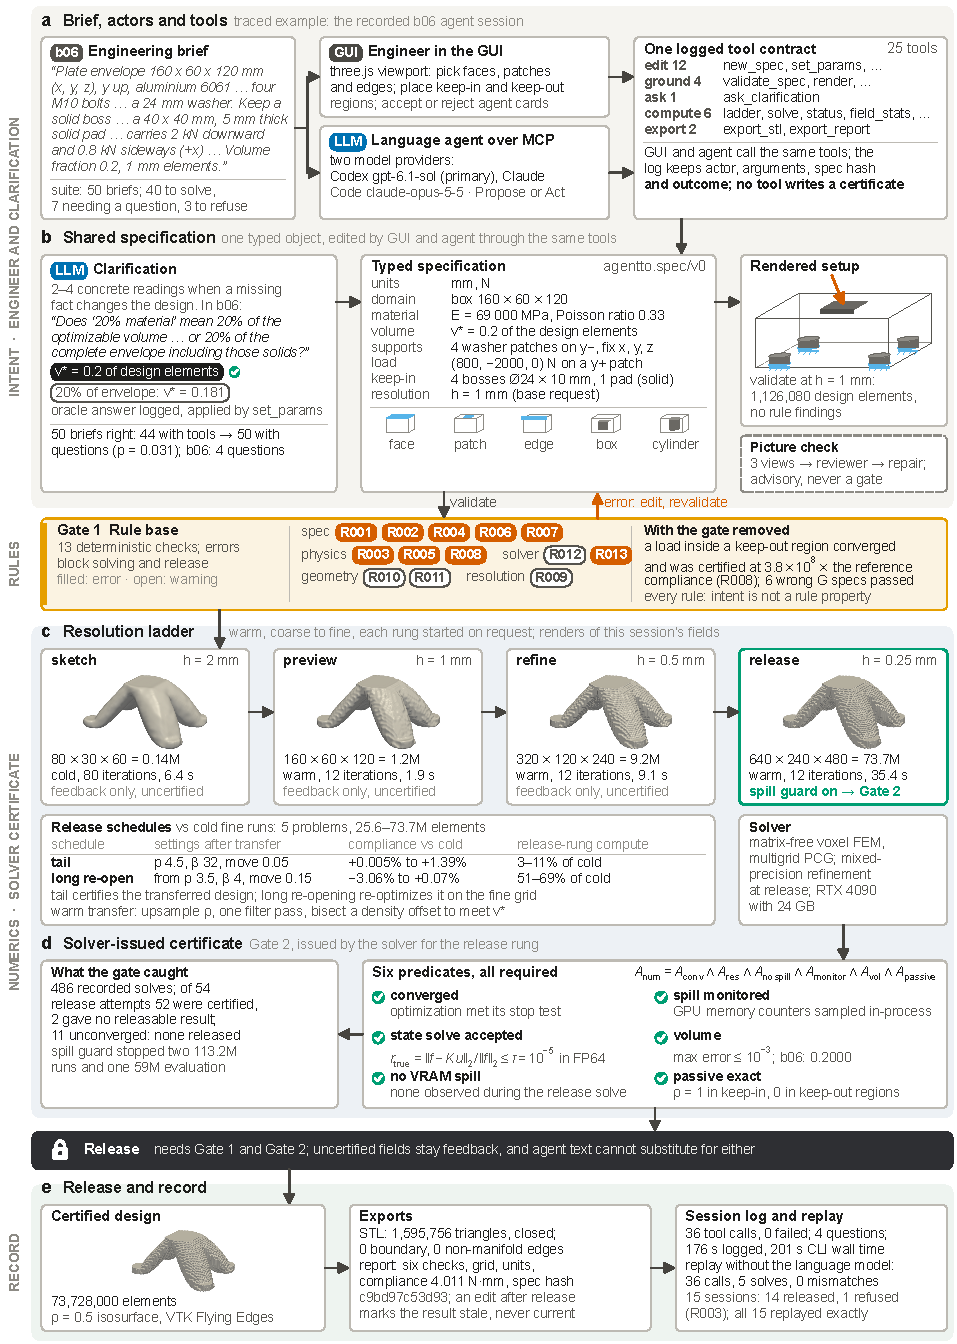
\includegraphics[width=156mm]{fig1_workflow.pdf}}
\caption{The AgenticTO workflow traced through one recorded agent session on the motor-mount brief b06, reproduced from
Figure~1 of the paper. The engineer and clarification settle intent, the rule gate admissibility and the solver
certificate numerical acceptance. Renders are $\rho=0.5$ isosurfaces of the saved fields; under the tail schedule the
fine rungs keep the transferred voxel steps.}
\label{fig:workflow}
\end{figure}

Figure~\ref{fig:workflow} follows one complete agent session through all of these pieces, from the brief to the
exported release. Chapter~\ref{ch:quickstart} repeats the same task by hand in the workspace.

\chapter{Installation and requirements}\label{ch:install}
\chapterintro{AgenticTO is a Python package with a web front end and a separate GPU solver. This chapter lists what you
need, installs the Python environment and the front end, connects the \code{voxfem} solver, and sets up the optional
language agents, which run on personal subscriptions only.}

\section{Requirements}\label{sec:requirements}

\begin{table}[h]
\caption{Requirements. ``Tested with'' is the configuration used for every result in the paper.}\label{tab:req}
\begin{fixtable}{@{}>{\raggedright\arraybackslash}p{0.2\linewidth}>{\raggedright\arraybackslash}p{0.27\linewidth}X@{}}
Item & Tested with & Notes \\ \midrule
GPU & NVIDIA GeForce RTX 4090, 24 GB & A CUDA 12 GPU. GPU memory bounds the finest grid you can release; rule
\rref{R013} estimates the memory before a solve starts. \\
Host & Intel Core i9-13900KF, 96 GB RAM & Large releases keep density fields in host memory as well. \\
Operating system & Windows 11 & The spill guard reads the Windows GPU-memory counters. Other platforms have not been
tested. \\
Python & 3.10 or newer (a conda environment) & See Section~\ref{sec:pyenv} for packages. \\
Node.js & 22 & Only for the web front end. \\
Solver & \code{voxfem} & Included in \code{src/voxfem/} (BSD 3-Clause; Section~\ref{sec:voxfem}). \\
Browser & Chrome & The workspace has been tested in Chrome with one user per session. \\
Codex CLI (optional) & 0.165.0, ChatGPT login & Runs the built-in assistant. \\
Claude Code (optional) & 2.1.312, claude.ai login & An external agent over MCP. \\
\end{fixtable}
\end{table}

\begin{notebox}[Shared desktop GPU]
In the paper the GPU also drove the desktop, and other processes held about 2--5~GB of its memory. That is why the
default ladder stops below \LadderMax\ elements, although a 24~GB card could hold more on its own. A guarded attempt at
$1.13\times10^{8}$ elements was stopped twice by the spill guard and is not part of any reported result
\claim{C3.2}.
\end{notebox}

\section{The Python environment}\label{sec:pyenv}
Create a conda environment with a CUDA 12 build of CuPy and the packages AgenticTO imports:

\begin{shell}
conda create -n agentto python=3.11
conda activate agentto
pip install numpy scipy matplotlib "cupy-cuda12x" "pydantic>=2.8,<3" \
    fastapi uvicorn mcp vtk pillow websockets pytest
\end{shell}

What each package is for: \code{numpy}, \code{scipy} and \code{cupy} for the numerics and \code{field\_stats};
\code{pydantic} for the specification schema and the tool arguments; \code{fastapi}, \code{uvicorn} and
\code{websockets} for the backend; \code{mcp} for the agent interface; \code{matplotlib} for the setup pictures of the
\tool{render} tool; \code{vtk} for the marching-cubes surface and the STL export; \code{pillow} for thumbnails.

Optional extras:
\begin{itemize}
  \item \code{pywin32} on Windows. The spill guard then reads the GPU memory counters in-process (about 0.1~ms per
  sample) instead of through a PowerShell subprocess (about 2.4~s per sample).
  \item \code{pyvista} for the 3D renders of the paper figures, \code{scikit-fem} for the independent cross-check of
  study X0, and \code{openpyxl} for the adjudication sheets (Chapter~\ref{ch:reproduce}).
\end{itemize}

AgenticTO is not installed into the environment. The scripts put \code{src/} on the Python path themselves, and the
MCP configurations in Chapter~\ref{ch:mcp} set \code{PYTHONPATH}. If you prefer an installed package,
\code{pip install -e .} in the repository root uses \code{pyproject.toml}.

\section{The web front end}
\begin{shell}
cd web
npm install
cd ..
\end{shell}
This installs React, three.js and Vite at the versions pinned in \code{web/package.json}.

\section{Connecting the solver}\label{sec:voxfem}
\index{voxfem@\code{voxfem}}\index{AGENTTO_VOXFEM_SRC@\code{AGENTTO\_VOXFEM\_SRC}}
AgenticTO runs on \code{voxfem}, the GPU solver of the authors' companion work on fused matrix-free operators,
Galerkin multigrid and guarded state solves. \code{voxfem} ships with the AgenticTO repository in \code{src/voxfem/}, unchanged and
under its own BSD 3-Clause License, and is found automatically when \code{src/} is on the path. AgenticTO imports it read-only, never writes into
it (no bytecode caches either), and extends it only by subclassing.

To use another copy of the solver, point AgenticTO at the directory that contains that \code{voxfem} package (the
directory you would put on \code{PYTHONPATH} to make \code{import voxfem} work):

\begin{shell}
# POSIX shell
export VOXFEM_SRC=/path/to/other/src
# Windows PowerShell
$env:VOXFEM_SRC = "D:/other/src"
\end{shell}

Set the variable in the shell that starts the backend, the MCP server or a script; the GPU worker inherits it.
The older name \code{AGENTTO\_VOXFEM\_SRC} still works.

\begin{warnbox}[Without a GPU]
Without a CUDA GPU you can still read the code, the briefs, the logs and every result file, and regenerate the
paper's tables and data figures from those files (Chapter~\ref{ch:reproduce}). Every solve needs a CUDA GPU.
\end{warnbox}

\section{Checking the installation}
\begin{shell}
python -B -m pytest -q
\end{shell}
The tests that solve on the GPU need a free GPU. Run one GPU job at a time: another CUDA program on the
same card can push a solve into shared memory, and the spill guard will then stop it.

\section{Optional: language agents on a subscription}\label{sec:agents}
\index{subscription policy}\index{PolicyError}
AgenticTO calls language models only through command-line tools that are logged in with a personal subscription:
the Codex CLI with a ChatGPT login for the built-in assistant, and optionally Claude Code with a claude.ai login.

\begin{shell}
codex login        # sign in with your ChatGPT account
claude             # the first run asks you to sign in with your claude.ai account
\end{shell}

Before every call AgenticTO checks two things, and refuses to start the agent if either fails:
\begin{enumerate}\sloppy
  \item No API-key variable is set: \code{OPENAI\_API\_KEY}, \code{CODEX\_API\_KEY}, \code{ANTHROPIC\_API\_KEY},
  \code{ANTHROPIC\_AUTH\_TOKEN}, \code{CLAUDE\_CODE\_USE\_BEDROCK} or \code{CLAUDE\_CODE\_USE\_VERTEX}. Any of them would
  silently switch billing to metered API use.
  \item The CLI is logged in with a subscription: \code{codex login status} must report ChatGPT, and
  \code{claude auth status} must report \code{claude.ai}.
\end{enumerate}
A refusal appears in the assistant panel as a \code{PolicyError}. Unset the variable, or log in again, and retry. The
child processes are started with those variables removed from their environment as a second safeguard.

The built-in assistant uses the model \code{gpt-6.1-sol} at reasoning effort high (the defaults in
\code{src/agentto/llm/cli.py}). Set \code{AGENTTO\_CODEX} or \code{AGENTTO\_CLAUDE} if the CLI is not on your
\code{PATH}.

\begin{tipbox}[The assistant is optional]
Every design in the paper's 50-brief suite can be built and solved in the workspace alone. The assistant and external
agents use the same tools you do.
\end{tipbox}

\chapter{Quick start: a certified release in ten minutes}\label{ch:quickstart}
\chapterintro{This chapter takes the motor-mount brief b06 from the task suite to a certified, exported design of
73.7 million elements. You start two processes, read the specification against the brief, climb the resolution
ladder, read the certificate and export the STL with its report. No language model is involved.}

\begin{notebox}[What you need]
A finished installation (Chapter~\ref{ch:install}) with the solver connected, and a GPU with about 24~GB of memory
that no other CUDA program is using. On a smaller GPU, start the backend with a lower ladder cap
(Section~\ref{sec:qs-small}); everything else in this chapter stays the same.
\end{notebox}

\section{The brief}
The brief is a plain-text file, \code{briefs/b06\_motor\_mount.md}:

\begin{quote}\small\sffamily
Plate envelope 160 x 60 x 120 mm (x, y, z), y up, aluminium 6061. It bolts to the machine bed through four M10 bolts on
its bottom face (y = 0) at x = 20 and 140 mm, z = 20 and 100 mm; each bolt clamps through a 24 mm washer. Keep a solid
boss of 24 mm diameter and 10 mm height around each bolt.

The motor sits on a 40 x 40 mm, 5 mm thick solid pad on the top face, centred at x = 80, z = 60. Its mounting pad
carries 2 kN downward and 0.8 kN sideways (+x) from belt tension.

Volume fraction 0.2, 1 mm elements.
\end{quote}

\section{Start the workspace}
\begin{steps}
\item Start the backend and its GPU worker. It listens on \code{127.0.0.1:8765}.
\begin{shell}
python -B scripts/serve.py
\end{shell}
\item In a second terminal, start the web front end:
\begin{shell}
node web/node_modules/vite/bin/vite.js web     # or: cd web && npm run dev
\end{shell}
\item Open \url{http://127.0.0.1:5173} in Chrome. The \gui{GPU} pill at the bottom right reads \emph{starting} until the
worker has loaded CUDA and the solver, then \emph{ready}.
\end{steps}

When the backend session is still empty, the workspace opens the suite task \code{b06\_motor\_mount} with its reference
specification, and shows the brief in the assistant panel. If the session already holds a design (the problem picker
then reads \gui{live session}), choose \gui{b06\_motor\_mount} in the problem picker at the top left.

\section{Read the specification against the brief}
Before solving anything, check that the specification says what the brief says. This is the intent check of
Section~\ref{sec:threechecks}, and no software can do it for you. The \gui{Design intent} tree on the left lists every
item; click one to see its exact values in the \gui{Inspector} and to highlight it in the viewport.
Table~\ref{tab:b06} maps the brief to the specification.

\begin{table}[h]
\caption{Brief b06 and its specification. Coordinates are absolute, in millimetres, with the origin at the domain's
minimum corner.}\label{tab:b06}
\begin{fixtable}{@{}>{\raggedright\arraybackslash}p{0.36\linewidth}>{\raggedright\arraybackslash}X@{}}
Brief & Specification \\ \midrule
envelope 160 x 60 x 120 mm, aluminium 6061 & domain \code{[160, 60, 120]}; material $E = 69000$~N/mm$^2$,
$\nu = 0.33$ \\
four M10 bolts through 24 mm washers on the bottom face & supports \code{bolt\_1}--\code{bolt\_4}: elliptical
\code{patch} regions of size 24 x 24 on face \code{y-}, centred at $(x,z)$ = (20, 20), (20, 100), (140, 20), (140, 100);
all directions fixed \\
solid boss, 24 mm diameter, 10 mm high & keep-in \code{boss\_1}--\code{boss\_4}: cylinders along $y$, radius 12,
span 0--10 \\
40 x 40 mm, 5 mm solid pad on top, centred at x = 80, z = 60 & keep-in \code{pad}: box from (60, 55, 40) to
(100, 60, 80) \\
2 kN down and 0.8 kN in +x on the pad & load \code{motor}: force \code{[800, -2000, 0]}~N on a 40 x 40 patch of face
\code{y+} \\
volume fraction 0.2, 1 mm elements & \code{volume\_fraction} 0.2 (of the design volume); resolution $h = 1$ \\
\end{fixtable}
\end{table}

The \gui{Checks} panel should read \emph{All rules pass}, and the top bar \emph{valid spec}. The ladder at the bottom
then shows four buttons.

\section{Climb the ladder}
The ladder for this specification has four named rungs. The spec's 1~mm elements are the base mesh; the release rung is
the finest grid that fits on the GPU, here 0.25~mm:

\begin{center}\small\sffamily
\begin{tabular}{@{}lrrl@{}}
\toprule
Rung & Element edge & Grid & Elements \\ \midrule
Sketch & 2 mm & 80 x 30 x 60 & 144,000 \\
Preview & 1 mm & 160 x 60 x 120 & 1.15 million \\
Refine & 0.5 mm & 320 x 120 x 240 & 9.2 million \\
Release & 0.25 mm & 640 x 240 x 480 & 73.7 million \\
\bottomrule
\end{tabular}
\end{center}

\begin{steps}
\item Click \gui{Sketch}. Density frames stream into the viewport while it runs. The first sketch of a new
specification builds its multigrid hierarchy and takes a few seconds; on the paper's workstation the cold b06 sketch
took 3.4~s.
\item Click \gui{Preview}, then \gui{Refine}. Each starts from the design of the rung below (marked \gui{$\uparrow$}
on the button) and takes seconds. Figure~\ref{fig:b06refine} shows the refine design.
\item When Refine has converged, click \gui{Optimize release}. It re-opens the optimization on the 73.7-million-element
grid for about 60 iterations. On the paper's workstation this policy used 61\% of the compute of a cold release-rung run
(423~s) and ended within 0.03\% of its compliance \claim{C3.1}. Alternatively, \gui{Release} certifies the upsampled
refine design in about 12 iterations (18~s of compute for b06 in the latency study \claim{C6.4}), but it barely changes
the design (Section~\ref{sec:policies}).
\end{steps}

\begin{figure}[t]
\wideshot{b06_refine.png}
\caption{The motor mount after Refine (9.2 million elements). The result card at the top right shows the checks: five
pass, but \emph{spill monitored} fails because spill monitoring runs only on the release rung, so the card says
\emph{not certified}. That is expected for every rung below Release. Screenshot from \code{scripts/gui\_screenshots.py}.}
\label{fig:b06refine}
\end{figure}

\section{Read the certificate}
When the release finishes, the result card shows the latest design and its certificate. A release is finished only
when the card reads \gui{certified}: all six checks carry a \pass, and the grid is the release grid (here
640 x 240 x 480). Chapter~\ref{ch:ladder} explains each check. The certified design is shown as its $\rho = 0.5$
surface; \gui{Voxels} switches to the raw density field.

\begin{figure}[t]
\centering
\shot[0.47\linewidth]{11_result_card.png}\hfill
\shot[0.47\linewidth]{13_export.png}
\caption{Left: the result card of a certified release, with all six checks passing. Right: the card after export,
with links to the STL and the two report files. These two screenshots come from the bracket of
Chapter~\ref{ch:spec} on a reduced ladder; the card for b06 has the same layout.}
\label{fig:qs-card}
\end{figure}

\section{Export}
Click \gui{Export STL + report}. Three files are written to the session's \code{exports/} folder, under
\code{sessions/}\meta{date-time}\code{/exports/}, and linked from the card (Figure~\ref{fig:qs-card}):

\begin{itemize}
  \item \code{b06\_motor\_mount\_}\meta{job}\code{.stl}: a closed binary STL of the full-resolution $\rho = 0.5$ surface
  (in the latency study the export at release took 0.3--2.2~s \claim{C6.4});
  \item \code{b06\_motor\_mount\_}\meta{job}\code{\_report.md} and \code{\_report.json}: the specification and its hash,
  the rung, grid and solver, iterations and compute time, the compliance, every certificate check, the STL's hash, and
  the hash of the session log at the moment of export (Appendix~\ref{app:certificate}).
\end{itemize}

A design that is not a certified release is exported with \code{\_draft} in its file name, so a draft cannot be
mistaken for a release later.

\begin{tipbox}[You are done]
You now hold a certified design, its STL, a report that ties it to the exact specification and solver settings, and a
session log in \code{sessions/}\meta{date-time}\code{/session.jsonl} from which the whole session can be replayed
(Chapter~\ref{ch:provenance}).
\end{tipbox}

\section{On a smaller GPU}\label{sec:qs-small}
Cap the ladder when you start the backend:
\begin{shell}
python -B scripts/serve.py --ladder-max 1.2e7
\end{shell}
The cap can lower the default of \LadderMax\ elements but never raise it. With this cap b06 gets the rungs 18,000 /
144,000 / 1.15 million / 9.2 million, and the 9.2-million-element rung becomes its release rung. The certificate means
the same on any rung that is the release rung of its ladder: the result is certified on the grid it reports, and the
report states that grid.

\section{The same task with an agent}
The paper ran this task without a person: a Codex agent connected over MCP built the specification from the brief,
asked four clarification questions (answered by a scripted oracle holding the reference reading), climbed the ladder and
exported a certified 73.7-million-element release in 176~s from its first tool call. Its specification equalled the
reference reading in every field, and the log replayed exactly. Chapter~\ref{ch:assistant} shows how to do the same with
the built-in assistant, and Chapter~\ref{ch:mcp} how to connect an agent of your own.

\chapter{The workspace}\label{ch:workspace}
\chapterintro{The workspace is a single browser page with ten areas. This chapter names each area, explains the status
indicators, and shows how to move around the 3D view. Later chapters use these names.}

\begin{figure}[t]
\centering
\widegraphic[178mm]{00_overview.png}
\caption{The workspace after a certified release of the bracket built in Chapter~\ref{ch:spec}. The numbers refer to
Table~\ref{tab:areas}.}
\label{fig:overview}
\end{figure}

\begin{table}[p]
\caption{The ten areas of the workspace (Figure~\ref{fig:overview}).}\label{tab:areas}
\begin{fixtable}{@{}c>{\raggedright\arraybackslash}p{0.2\linewidth}X@{}}
\# & Area & What it does \\ \midrule
\callout{1} & \gui{Top bar} & Problem picker (\gui{New design\ldots}, the 50 suite tasks, the three template problems),
specification status, backend connection and round-trip time, light/dark theme. \\
\callout{2} & \gui{Design intent} & The specification as a tree: domain, material, supports, loads, keep-in and keep-out
regions. Click an item to select it; a red \gui{error} or amber \gui{check} badge marks an item that a rule flags. \\
\callout{3} & \gui{Checks} & Live rule findings, each with its code, severity and message. \\
\callout{4} & \gui{Inspector} & Exact values of the selected item, edited in place: region kind, face, centre, size,
force, fixed directions. \\
\callout{5} & \gui{Viewport tools} & \gui{Select}, \gui{Support}, \gui{Load}, \gui{Keep-in}, \gui{Keep-out};
\gui{Hide design}. \\
\callout{6} & \gui{3D viewport} & The domain with supports (blue), loads (orange arrows), keep-in (green) and keep-out
(pink) regions; the density design or its surface; the orientation cube; a size legend. \\
\callout{7} & \gui{Result card} & The latest finished design: certified or not, current or stale, compliance, volume,
grid, each certificate check, \gui{Surface}/\gui{Voxels}, \gui{Export STL + report}. \\
\callout{8} & \gui{Assistant} & Chat with the design assistant, the \gui{Propose}/\gui{Act} dial, clarification
questions and proposed changes as cards. \\
\callout{9} & \gui{Resolution ladder} & \gui{Sketch}, \gui{Preview}, \gui{Refine} and \gui{Release} with their element
counts, times and certificate seals; \gui{Optimize release}; \gui{Stop}; live compliance and volume with a convergence
sparkline; the \gui{GPU} status pill. \\
\callout{10} & \gui{Timeline} & The session log, newest on the right, each record tagged \gui{USER}, \gui{AGENT},
\gui{GPU} or \gui{SYSTEM}. Hover a record for its time and details. \\
\end{fixtable}
\end{table}

\section{The areas}
Figure~\ref{fig:overview} and Table~\ref{tab:areas} name the ten areas. Three of them carry most of the work: the
\gui{Design intent} tree with its \gui{Inspector} below (where you state the problem), the viewport (where you place
regions by clicking faces), and the ladder with the result card (where you solve and read the outcome).

\section{Status indicators}
\begin{description}
  \item[Specification status] (top bar). \emph{valid spec}, \emph{valid $\cdot$ $n$ warnings}, or \emph{$n$ errors}.
  It counts rule findings and schema errors. The ladder is hidden or disabled while there is an error.
  \item[Backend] (top bar). Whether the WebSocket to the backend is open, with the round-trip time in milliseconds.
  \item[GPU] (bottom right). \emph{off} before the first solve request, \emph{starting} while the worker process loads
  CUDA and the solver, \emph{ready}, or \emph{dead} if the worker exited (Chapter~\ref{ch:limits}).
  \item[Rung buttons]. Each shows its element count and, after a solve, its compute time; an \gui{$\uparrow$} marks a warm
  start from the rung below, a seal marks a certified result. While a rung runs it shows \emph{setting up\ldots} and then
  the iteration count.
  \item[Result card badges]. \gui{certified} or \gui{not certified}, and \gui{stale} when the specification has changed
  since this design was solved (Section~\ref{sec:stale}).
\end{description}

\section{First launch}
On first launch a \gui{Getting started} card sits above the result card (Figure~\ref{fig:firstrun}). It summarizes the
workflow in three steps and the two shortcuts worth learning first: \keycap{?} for the keyboard map and
\keycap{Ctrl}+\keycap{K} for the command palette. \gui{Got it} hides it.

\begin{figure}[t]
\wideshot{01_first_run.png}
\caption{The \gui{Getting started} card at the top right. In this screenshot the backend session already held the
bracket of Chapter~\ref{ch:spec}, so the problem picker reads \gui{live session}; on an empty session the workspace opens
the suite task b06 instead.}
\label{fig:firstrun}
\end{figure}

\section{Moving around the 3D view}
\index{viewport navigation}
\begin{itemize}
  \item Left-drag orbits, right-drag pans, the mouse wheel zooms.
  \item Click a face of the orientation cube to look along that axis.
  \item Click an item in the viewport or in the tree to select it; the inspector shows its values.
  \item \gui{Hide design} hides the density so you can see the regions inside it.
\end{itemize}

\section{The timeline}
The timeline at the bottom is the session log made visible (Figure~\ref{fig:timeline}). Each record is a tool call or a
solve result, tagged with its actor. Agent edits appear here just like yours. Chapter~\ref{ch:provenance} describes the
log behind it.

\begin{figure}[h]
\widegraphic[178mm]{15_timeline.png}
\caption{The timeline: user edits, solves and GPU results, each tagged with its actor.}
\label{fig:timeline}
\end{figure}

\section{Themes, keyboard and palette}
\gui{Dark}/\gui{Light} in the top bar switches the theme (Figure~\ref{fig:dark}). \keycap{?} opens the keyboard map and
\keycap{Ctrl}+\keycap{K} the command palette, which runs any rung, \gui{Optimize release}, \gui{Stop}, shows the last
surface, exports, undoes and redoes, picks a tool and switches the theme. Appendix~\ref{app:keys} lists all shortcuts.
Shortcuts are off while you type in a field.

\begin{figure}[h]
\wideshot[150mm]{18_dark.png}
\caption{The dark theme.}
\label{fig:dark}
\end{figure}

\chapter{Building a specification}\label{ch:spec}
\chapterintro{The specification is the one document that says what problem is solved. This chapter builds one by hand
in the workspace, a small steel bracket with a solid pad and a bolt hole, and then explains each part of the document:
the coordinate frame, units, material, supports, loads, keep-in and keep-out regions, the volume fraction and the
mesh.}

\section{Tutorial: a cantilever bracket}\label{sec:tutorial}
The bracket is a 100 x 50 x 50~mm steel block, fixed at one end and loaded at the other, with a mounting pad that must
stay solid and a hole that must stay empty. The screenshots were recorded with the ladder capped at
$1.2\times10^{7}$ elements, so that the release solves in about a minute.

\subsection{Start a new design}
Choose \gui{New design\ldots} in the problem picker. You get an empty 100 x 50 x 50~mm box in steel ($E = 210000$,
$\nu = 0.3$, in N and mm) with a volume fraction of 0.3 and 20 elements along the shortest edge. The \gui{Checks} panel
says what is missing, and the ladder stays hidden until the specification is valid (Figure~\ref{fig:newdesign}).

\begin{figure}[t]
\wideshot{02_new_design.png}
\caption{A new design. The checks say what is missing and how to add it.}
\label{fig:newdesign}
\end{figure}

Select \gui{Domain} in the tree to set the size, the units, the volume fraction (\gui{volume \%}), the mesh (by element
size $h$ or by cells along the shortest edge) and an optional minimum feature size. Select \gui{Material} to set its
name, Young's modulus $E$ and Poisson's ratio $\nu$.

\subsection{Add a support}
Press \keycap{S} (or click \gui{Support}) to arm the support tool. The toolbar asks you to click a face of the domain
(Figure~\ref{fig:supporttool}). Click the face at $x = 0$. It becomes a support fixed in all three directions, the tool
returns to \gui{Select}, and the new support is selected in the inspector. There you can change the region kind (face,
patch, edge, box or cylinder) and untick fixed directions to make a roller.

\begin{figure}[t]
\wideshot{03_support_tool.png}
\caption{The support tool armed: click the face to fix.}
\label{fig:supporttool}
\end{figure}

\subsection{Add a load}
Press \keycap{L} and click the face at $x = 100$. A 1~kN load appears on a small patch centred where you clicked,
pointing into the face. Edit it in the inspector: here the force becomes 2000~N downward (force $y = -2000$) and the
patch 10 x 20~mm (Figure~\ref{fig:loadinspector}). Each edit takes effect as you type and can be undone.

\begin{figure}[t]
\wideshot{04_load_inspector.png}
\caption{A load placed by clicking and then edited in the inspector.}
\label{fig:loadinspector}
\end{figure}

\subsection{When a check fails}
The rules run \CheckDelay~ms after every edit. Untick $y$ and $z$ on the support, so that it fixes only $x$: rule
\rref{R003} reports the rigid-body motions left free (translation in $y$ and $z$, rotation about $x$), the support gets
an \gui{error} badge in the tree, and the ladder locks (Figure~\ref{fig:ruleerror}). Tick $y$ and $z$ again and the error
clears. Errors block solving; warnings and notes do not.

\begin{figure}[t]
\centering
\shot[0.30\linewidth]{06_rule_error.png}
\caption{Rule R003: the support leaves rigid-body motion free. The ladder stays locked until the support is fixed.}
\label{fig:ruleerror}
\end{figure}

\subsection{Keep-in and keep-out regions}
Press \keycap{K} and click a face to add a keep-in region (always solid), or \keycap{O} for a keep-out region (always
empty). Each starts as a slab 10\% thick against that face. In the inspector a keep-in or keep-out region can be a box
or a cylinder, and you can switch it between keep-in and keep-out.

In Figure~\ref{fig:keep} the keep-in region was resized to an 8 x 20 x 30~mm pad under the load, using its min/max
fields. The keep-out region was converted to a cylinder of radius 8~mm along $z$, centred at $x = 40$, which leaves a
through-hole for a bolt or a cable.

\begin{figure}[t]
\wideshot{05_keepin_keepout.png}
\caption{The finished setup: support (blue), load on a solid pad (green) and a keep-out cylinder (pink). All rules
pass.}
\label{fig:keep}
\end{figure}

\subsection{Undo and redo}
\keycap{Ctrl}+\keycap{Z} undoes and \keycap{Ctrl}+\keycap{Shift}+\keycap{Z} or \keycap{Ctrl}+\keycap{Y} redoes, across
your edits and agent edits alike. Every step is a record in the timeline. Chapter~\ref{ch:ladder} continues with this
bracket and solves it.

\section{The document}\label{sec:document}
\index{specification!document}
Whatever you do in the workspace ends up as one JSON document. This is the reference specification of suite task b01:

\begin{jsoncode}
{
  "schema_version": "agentto.spec/v0",
  "name": "b01 cantilever block",
  "units": {"length": "mm", "force": "N"},
  "domain": {"size": [200, 100, 100]},
  "material": {"name": "steel", "E": 210000.0, "nu": 0.3},
  "volume_fraction": 0.3,
  "supports": [{"id": "wall", "region": {"kind": "face", "face": "x-"}}],
  "loads": [{"id": "pad", "force": [0, -1000, 0],
             "region": {"kind": "patch", "face": "x+", "center": [50, 50],
                        "size": [10, 10], "shape": "rect"}}],
  "passive": [],
  "resolution": {"h": 1.0}
}
\end{jsoncode}

The schema is strict: unknown fields are rejected, every \code{id} must be unique across supports, loads and passive
regions, and a document needs at least one support, one load, a volume fraction and a resolution. A draft that is not
complete yet (no load, say) is kept as a draft; the tools report what is missing and the rules do not run until it is
complete. Appendix~\ref{app:spec} lists every field.

\subsection{Coordinate frame}
\index{coordinate frame}
The domain is an axis-aligned box from $(0,0,0)$ to the size you give. All coordinates are absolute, in that frame. The
faces are named \code{x-}, \code{x+}, \code{y-}, \code{y+}, \code{z-} and \code{z+}: \code{x-} is the face at $x = 0$,
\code{x+} the face at $x = L_x$. Which axis is ``up'' is yours to choose; the brief b06, for example, says ``y up''.

A patch on a face gives its centre and full size in the face's two in-plane axes, always in increasing axis order:
$(y,z)$ on $x$ faces, $(x,z)$ on $y$ faces, $(x,y)$ on $z$ faces. This is the most common source of misplaced regions.
\tool{list_regions} prints the in-plane axes of every face, and the viewport shows the result.

\subsection{Units}
\index{units}
Lengths are in mm, m or in; forces in N, kN or lbf. The units label the numbers; they do not convert them.

\begin{warnbox}[Units relabel; they do not convert]
Switching from mm to m changes the label on the numbers, not the numbers. Enter every value in the units shown, and
keep $E$ consistent with them: in N and mm, $E$ is in N/mm$^2$ (MPa), so steel is 210000. In kN and mm, steel is 210. In
the paper's second-provider benchmark, two of the four remaining wrong answers were exactly this slip: the agent worked
in kN and mm but left $E$ in MPa, a material 1000 times too stiff.
\end{warnbox}

\subsection{Material}
An isotropic linear-elastic material: a name, $E$ (positive) and $\nu$ (between $-1$ and $0.5$). The name is a label;
only $E$ and $\nu$ enter the computation. Because the objective is compliance under one load case, the optimal layout
does not depend on $E$, but the reported compliance does, and the specification must state the problem the engineer
meant.

\subsection{Regions}\label{sec:regions}
\index{regions}
Supports and loads select grid \emph{nodes}; keep-in and keep-out regions select \emph{elements} by their centres.
Table~\ref{tab:regions} lists the five region kinds.

\begin{table}[h]
\caption{Region kinds. All lengths are in the spec's length unit; ``in-plane order'' is the increasing axis order of
the face's two in-plane axes.}\label{tab:regions}
\begin{fixtable}{@{}l>{\raggedright\arraybackslash}X>{\raggedright\arraybackslash}p{0.26\linewidth}@{}}
Kind & Fields & Valid for \\ \midrule
\code{face} & \code{face}: one of \code{x-}, \code{x+}, \code{y-}, \code{y+}, \code{z-}, \code{z+} & supports, loads \\
\code{patch} & \code{face}; \code{center} and \code{size} in in-plane order; \code{shape} \code{rect} (default) or
\code{ellipse} (the inscribed ellipse, e.g. a washer) & supports, loads \\
\code{edge} & \code{axis}; \code{at}: the other two coordinates in increasing order; optional \code{span} [start, end]
along the axis & supports, loads \\
\code{box} & \code{min}, \code{max}: opposite corners, \code{min} $<$ \code{max} on every axis & supports, loads,
keep-in/out \\
\code{cylinder} & \code{axis}; \code{center}: the axis position in the other two coordinates; \code{radius};
\code{span} [start, end] along the axis & supports, loads, keep-in/out \\
\end{fixtable}
\end{table}

Selection uses a rounding tolerance of $10^{-9}$ element edges. A patch with no node within half its size of its
centre, or an edge between grid lines, is snapped to the nearest grid line and reported by rule \rref{R010}; nothing is
snapped silently. A region that selects nothing is an error (\rref{R002} for a support, \rref{R004} for a load) or a
warning (\rref{R011} for a passive region).

\subsection{Supports}
A support fixes the nodes of its region in the directions listed in \code{fix}; the default is all three. A roller
fixes fewer: \code{"fix": ["y"]} on a bottom edge leaves the span and width directions free. Supports only need to
remove the six rigid-body modes together; rule \rref{R003} checks exactly that.

\subsection{Loads}
A load is a total force vector, in the spec's force unit, shared equally by the nodes of its region. This keeps the
total force the same on every mesh, but it is not a pressure integration: on a curved or partial region the nodal
shares are equal, not area-weighted. All loads act together as one load case. A load component that falls on a fixed
degree of freedom is dropped, because it would go straight into the support, and rule \rref{R005} reports the share.

\subsection{Keep-in and keep-out regions}
\index{keep-in region}\index{keep-out region}\index{passive region|see{keep-in region, keep-out region}}
In the document these are \code{passive} items with \code{kind} \code{solid} (keep-in) or \code{void} (keep-out), each
a box or a cylinder. An element whose centre falls inside is held at density 1 or 0 at every iteration and is not a
design variable. Keep-out elements keep a small stiffness rather than zero, so their nodes stay well defined. The
certificate checks that every keep-in element ends at exactly 1 and every keep-out element at exactly 0.

\subsection{Volume fraction}\label{sec:vf}
\index{volume fraction}
The volume fraction $v^*$ is the share of the \emph{design} volume, which is the domain minus every keep-in and keep-out
element:
\begin{equation}
  \frac{1}{|\mathcal D|}\sum_{e\in\mathcal D}\bar\rho_e \le v^*,\qquad \bar\rho_e = 1\ (e\in\mathcal S),\quad
  \bar\rho_e = 0\ (e\in\mathcal V),
\end{equation}
where $\mathcal D$ are the design elements, $\mathcal S$ the keep-in and $\mathcal V$ the keep-out elements, and
$\bar\rho$ the filtered and projected density. Adding a keep-in pad therefore adds material on top of the budget; it
changes both the feasible set and the total material. That is why an agent that invents a pad the brief did not ask for
has changed the problem, even if the result looks stiffer.

\subsection{Resolution and the minimum feature}
\index{resolution}
Give the mesh as an element edge \code{h} or as \code{cells\_short\_edge}, the number of elements along the shortest
side; exactly one of the two. The edge must divide all three sides into whole numbers of elements, or rule \rref{R001}
fires. This resolution is the \emph{base} mesh from which the ladder is built. The release rung is the finest rung that
fits on the GPU and is often finer: for b06 the spec says 1~mm and the release rung is 0.25~mm
(Section~\ref{sec:rungs}).

The optional \code{min\_feature} is the smallest member you need. It does not constrain the optimizer; it only feeds
rule \rref{R009}, which warns when that size spans fewer than about 2.4 elements and would be filtered out.

\section{Editing through the tools}\label{sec:editing}
Every edit in the workspace is a call to one of the editing tools, logged like an agent's call. The same calls work from
Python and over MCP:

\begin{itemize}
  \item \tool{new_spec} starts a box domain; \tool{set_spec} replaces the whole document.
  \item \tool{set_params} sets scalar fields (name, size, units, $E$, $\nu$, material name, volume fraction, $h$ or
  \code{cells\_short\_edge}, \code{min\_feature}); only the arguments given change.
  \item \tool{add_support}, \tool{add_load} and \tool{add_passive} add items; \tool{update_item} changes fields of one;
  \tool{remove_item} deletes one.
  \item \tool{undo} and \tool{redo} step through the history.
\end{itemize}

A failed edit leaves the specification unchanged. Every successful edit is undoable and records the hash of the
resulting specification in the log, so any later result can be tied to the exact document it was solved from.

\begin{tipbox}[Ground before you solve]
\tool{list_regions} reports, for every item, its physical bounding box and how many nodes or elements it selects at a
given mesh, with any snapping. \tool{explain_spec} prints the whole specification in plain sentences, and
\tool{render} draws the supports, loads and passive regions as a picture. All three are cheap; use them before the
first solve.
\end{tipbox}

\chapter{Rules}\label{ch:rules}
\chapterintro{Thirteen deterministic rules check that a specification states an admissible problem before anything is
solved. This chapter explains when the rules run, how to read a finding, and what each code means and how to fix it.
The rule list in this chapter is generated from \code{src/agentto/rules.py}.}

\section{When the rules run}
\index{rules!when they run}
\begin{itemize}
  \item In the workspace, \CheckDelay~ms after the last edit. In the paper's latency study the 95th-percentile
  validation time per task was 1.2--10.5~ms \claim{C6.4}.
  \item On every \tool{validate_spec} call, at the specification's own mesh or at a mesh size \code{h} you pass.
  \item On every \tool{solve} call, again at the mesh of the requested rung. A solve whose rung fails validation is
  refused before it reaches the GPU, and the GPU worker checks once more before it starts.
\end{itemize}

Any \sev{error} blocks solving and release. A \sev{warning} or \sev{info} finding does not block; it stays visible in
the \gui{Checks} panel, often with a suggested fix. Several rules depend on the grid (for example R002, R010, R011 and
R013), so a specification can pass at one mesh and fail at another.

\section{Reading a finding}
Each finding has a stable code, a severity, a message, the ids of the items it concerns (the tree marks those items),
and, where one exists, a fix. A fix either sets a field (the workspace can offer it as one click, and an agent can
propose it as a card) or suggests an action in words. \tool{validate_spec} returns the findings as JSON:

\begin{jsoncode}
{"ok": false,
 "resolution": {"h": 1.0, "grid": [100, 50, 50], "n_elem": 250000, ...},
 "findings": [{"code": "R003", "severity": "error",
   "message": "supports leave rigid-body motion free: translation y, translation z, rotation about x",
   "ids": ["support_1"],
   "fix": {"suggest": "add a support that restrains translation y, translation z, rotation about x"}}]}
\end{jsoncode}

The codes are stable: experiments, logs and this book refer to them, and a code is never reused for a different
check.

\section{Summary}
% Generated by docs/guidebook/gen_tables.py from the code. Do not edit by hand.
\begin{reftable}{@{}l>{\raggedright\arraybackslash}p{0.2\linewidth}X@{}}
Code & Severity & Fires when \\ \midrule
\hyperref[rule:R001]{\textbf{R001}} & \sev{error} & no grid fits the domain at this element size \\
\hyperref[rule:R002]{\textbf{R002}} & \sev{error} & a support selects no nodes \\
\hyperref[rule:R003]{\textbf{R003}} & \sev{error} & the supports leave a rigid-body mode free \\
\hyperref[rule:R004]{\textbf{R004}} & \sev{error} & a load selects no nodes, or every load is zero \\
\hyperref[rule:R005]{\textbf{R005}} & \sev{error} / \sev{warning} & part of the load acts on fixed degrees of freedom \\
\hyperref[rule:R006]{\textbf{R006}} & \sev{error} & no design elements remain \\
\hyperref[rule:R007]{\textbf{R007}} & \sev{error} & elements are both keep-in and keep-out \\
\hyperref[rule:R008]{\textbf{R008}} & \sev{error} & a support or load lies entirely inside a keep-out region \\
\hyperref[rule:R009]{\textbf{R009}} & \sev{warning} & the minimum feature is not resolvable at this mesh \\
\hyperref[rule:R010]{\textbf{R010}} & \sev{warning} & a region was snapped to the grid \\
\hyperref[rule:R011]{\textbf{R011}} & \sev{warning} & a passive region contains no element centre \\
\hyperref[rule:R012]{\textbf{R012}} & \sev{warning} / \sev{info} & supports change on the coarsest multigrid level \\
\hyperref[rule:R013]{\textbf{R013}} & \sev{error} & the grid needs more GPU memory than is available \\
\end{reftable}


\section{Rule by rule}
In the messages below, \meta{id} and similar placeholders stand for values filled in at run time.

% Generated by docs/guidebook/gen_tables.py from the code. Do not edit by hand.
\begin{rulecard}{R001}{\sev{error}}{no grid fits the domain at this element size}\label{rule:R001}\index{R001@\texttt{R001} (rule)}
\rulefield{Message}\msgline{domain \meta{axis} size \meta{length} is not a whole number of elements of edge \meta{h}}
\rulefield{Meaning}A side of the domain is not a whole number of elements of edge $h$ (or the number of cells along the short edge gives a non-integer count on another side). R001 stops the check: no other rule runs until a grid exists.
\rulefield{Fix}Choose an $h$ that divides all three sides, or accept the one-click fix, which sets \code{cells\_short\_edge} to a value that fits. \emph{(The finding carries a fix: one click: set \code{resolution.cells\_\allowbreak{}short\_\allowbreak{}edge}.)}
\end{rulecard}

\begin{rulecard}{R002}{\sev{error}}{a support selects no nodes}\label{rule:R002}\index{R002@\texttt{R002} (rule)}
\rulefield{Message}\msgline{support '\meta{id}' selects no nodes}
\rulefield{Meaning}The support's region misses every grid node: a box between grid planes, a cylinder thinner than the node spacing, an edge span outside the domain. The support does nothing.
\rulefield{Fix}Run \code{list\_regions} to see the node count of each item, then move or enlarge the region, or refine the mesh.
\end{rulecard}

\begin{rulecard}{R003}{\sev{error}}{the supports leave a rigid-body mode free}\label{rule:R003}\index{R003@\texttt{R003} (rule)}
\rulefield{Message}\msgline{supports leave rigid-body motion free: \meta{modes}}
\rulefield{Meaning}The fixed degrees of freedom do not remove all six rigid-body modes, so the stiffness matrix is singular. The message names the free translations and rotations. A common cause is a single edge support (free rotation about the edge) or rollers that fix only one direction.
\rulefield{Fix}Add a support, or fix more directions, so that the listed modes are restrained. Fix in the spec; do not rely on the solver to fail. \emph{(The finding carries a fix: suggests: add a support that restrains \meta{modes}.)}
\end{rulecard}

\begin{rulecard}{R004}{\sev{error}}{a load selects no nodes, or every load is zero}\label{rule:R004}\index{R004@\texttt{R004} (rule)}
\rulefield{Message}\msgline{every load has zero force} \newline \msgline{load '\meta{id}' selects no nodes}
\rulefield{Meaning}Either a load region misses every node, or the force vectors of all loads are zero, so there is nothing to optimize against.
\rulefield{Fix}Check the load's region with \code{list\_regions} and its force components with \code{explain\_spec}.
\end{rulecard}

\begin{rulecard}{R005}{\sev{error} / \sev{warning}}{part of the load acts on fixed degrees of freedom}\label{rule:R005}\index{R005@\texttt{R005} (rule)}
\rulefield{Message}\msgline{\meta{share}\% of the applied load acts on fixed DOFs and is lost}
\rulefield{Meaning}The problem builder drops every load component that falls on a fixed degree of freedom (it would go straight into the support) and records the share. Above 50\% of the load the finding is an error, otherwise a warning.
\rulefield{Fix}Move the load off the support, or leave that direction free at the shared nodes.
\end{rulecard}

\begin{rulecard}{R006}{\sev{error}}{no design elements remain}\label{rule:R006}\index{R006@\texttt{R006} (rule)}
\rulefield{Message}\msgline{no design elements remain after passive regions}
\rulefield{Meaning}The keep-in and keep-out regions together cover every element, so there is nothing to design.
\rulefield{Fix}Shrink or remove passive regions.
\end{rulecard}

\begin{rulecard}{R007}{\sev{error}}{elements are both keep-in and keep-out}\label{rule:R007}\index{R007@\texttt{R007} (rule)}
\rulefield{Message}\msgline{\meta{n} elements are both keep-in and keep-out}
\rulefield{Meaning}A keep-in and a keep-out region overlap. An element cannot be held solid and empty at once.
\rulefield{Fix}Remove the overlap: shrink one region, or split it.
\end{rulecard}

\begin{rulecard}{R008}{\sev{error}}{a support or load lies entirely inside a keep-out region}\label{rule:R008}\index{R008@\texttt{R008} (rule)}
\rulefield{Message}\msgline{\meta{support\textbar{}load} '\meta{id}' lies entirely inside a keep-out region}
\rulefield{Meaning}Every element around the item's nodes is held empty, so the load has no material path (or the support holds nothing). The solver can still converge on such a problem because empty elements keep a small stiffness; in the paper's gate ablation it converged and passed the numerical certificate.
\rulefield{Fix}Move the item out of the keep-out region, or move the keep-out region.
\end{rulecard}

\begin{rulecard}{R009}{\sev{warning}}{the minimum feature is not resolvable at this mesh}\label{rule:R009}\index{R009@\texttt{R009} (rule)}
\rulefield{Message}\msgline{min feature \meta{min feature} is \meta{n} elements; members below about \meta{2.4} elements are filtered out}
\rulefield{Meaning}\code{min\_feature} spans fewer than about 2.4 elements (twice the final filter radius of 1.2 elements); members that thin are filtered out.
\rulefield{Fix}Accept the one-click fix, which sets $h$ to \code{min\_feature}/2.4, or relax \code{min\_feature}. \emph{(The finding carries a fix: one click: set \code{resolution.h}.)}
\end{rulecard}

\begin{rulecard}{R010}{\sev{warning}}{a region was snapped to the grid}\label{rule:R010}\index{R010@\texttt{R010} (rule)}
\rulefield{Message}\msgline{\meta{n}}
\rulefield{Meaning}A patch had no node within half its size of its centre, or an edge fell between grid lines; it was moved to the nearest grid line. Nothing is snapped silently.
\rulefield{Fix}Usually harmless. If the change matters, align the coordinates with the grid or refine the mesh.
\end{rulecard}

\begin{rulecard}{R011}{\sev{warning}}{a passive region contains no element centre}\label{rule:R011}\index{R011@\texttt{R011} (rule)}
\rulefield{Message}\msgline{passive region '\meta{id}' contains no element centre at h=\meta{h}}
\rulefield{Meaning}At this element size no element centre falls inside the keep-in or keep-out region, so it has no effect.
\rulefield{Fix}Refine the mesh or enlarge the region. \emph{(The finding carries a fix: suggests: refine the mesh or enlarge the region.)}
\end{rulecard}

\begin{rulecard}{R012}{\sev{warning} / \sev{info}}{supports change on the coarsest multigrid level}\label{rule:R012}\index{R012@\texttt{R012} (rule)}
\rulefield{Message}\msgline{on the coarsest multigrid level (1/\meta{stride} resolution) the supports leave rigid modes free (\meta{modes}); the solver switches to the dilated coarse support rule (RobustGMG)} \newline \msgline{supports \meta{ids} are not represented on the coarsest multigrid level (1/\meta{stride}); the solve stays correct but may need more iterations}
\rulefield{Meaning}On the coarsest multigrid level the supports either leave rigid modes free (warning: the solver switches to the dilated coarse support rule) or lose some supports (info: the solve stays correct but may need more iterations). Neither blocks solving.
\rulefield{Fix}No action is needed. The finding explains a slower solve.
\end{rulecard}

\begin{rulecard}{R013}{\sev{error}}{the grid needs more GPU memory than is available}\label{rule:R013}\index{R013@\texttt{R013} (rule)}
\rulefield{Message}\msgline{\meta{g.n\_elem / 1000000.0}M elements need about \meta{need / 1000000000.0} GB with \meta{solver}; the GPU has \meta{vram\_bytes / 1000000000.0} GB}
\rulefield{Meaning}The memory estimate (bytes per element times elements) exceeds the GPU memory. The estimate uses about 366 bytes per element for \code{mg64} and 146 for \code{mg\_ir}.
\rulefield{Fix}Solve a coarser rung. A solve checks with \code{mg\_ir}; validation at the spec's own mesh checks with \code{mg64}. \emph{(The finding carries a fix: suggests: use mg\_ir or a coarser rung.)}
\end{rulecard}


\section{What the rules cannot see}\label{sec:rulelimits}
The rules decide whether a problem is admissible, not whether it is the problem the engineer meant. A support that
selects real nodes and removes every rigid-body mode passes, even if it restrains a direction the brief leaves free. A
keep-in pad that the brief never mentioned passes. A load with the right magnitude on the wrong face passes. These are
intent errors, and only the engineer, helped by clarification, can catch them (Chapter~\ref{ch:assistant}).

\begin{evidencebox}
With grounding tools but no questions, the primary agent produced 6 wrong specifications on the 50-brief suite. All 6
passed every rule \claim{C4.2}. Conversely, the rules stopped all 3 deliberately ill-posed briefs before any solve: two
rigid-body cases (\rref{R003}) and one load inside its own keep-out region (\rref{R008}) \claim{C4.1}.
\end{evidencebox}

The rules also do not check that the final design is connected, that the exported surface is manufacturable, or that
the structure is safe. The release certificate (Chapter~\ref{ch:ladder}) covers the numerical computation, and nothing
in AgenticTO covers structural safety.

\chapter{The resolution ladder and the release certificate}\label{ch:ladder}
\chapterintro{A specification is solved on a ladder of grids, each twice as fine per axis as the one below. This chapter
explains how the rungs are chosen, how one rung starts from the design of the one below, the three warm release
policies and what each can and cannot do, and the six predicates of the release certificate.}

\section{The rungs}\label{sec:rungs}
\index{resolution ladder}\index{rung}
The ladder is built from the specification's base mesh $h$. Candidate element sizes are $h\cdot 2^k$ for integer
$k$; a candidate is kept when its grid divides the domain into whole elements and has between \LadderMin\ and
\LadderMax\ elements. Consecutive rungs must differ by exactly a factor of two per axis, so that every rung can start
from the one below. The four finest rungs are named \emph{sketch}, \emph{preview}, \emph{refine} and \emph{release};
any coarser ones are named \code{coarse0}, \code{coarse1}, \ldots{} and are not shown in the workspace.

\begin{figure}[h]
\centering
\begin{tikzpicture}[font=\sffamily\footnotesize,
  rung/.style={draw=#1,fill=#1!10,line width=0.7pt,rounded corners=1.5pt,minimum height=9mm,align=center},
  arr/.style={-{Stealth[length=2mm]},line width=0.6pt,color=guigrey}]
  \node[rung=guigrey,minimum width=20mm] (s) {\textbf{Sketch}\\144k};
  \node[rung=guigrey,minimum width=24mm,right=7mm of s] (p) {\textbf{Preview}\\1.15M};
  \node[rung=guigrey,minimum width=28mm,right=7mm of p] (r) {\textbf{Refine}\\9.2M};
  \node[rung=okgreen,minimum width=34mm,right=7mm of r] (R) {\textbf{Release}\\73.7M, spill guard on};
  \draw[arr] (s) -- node[above,font=\scriptsize\sffamily]{warm} (p);
  \draw[arr] (p) -- node[above,font=\scriptsize\sffamily]{warm} (r);
  \draw[arr] (r) -- node[above,font=\scriptsize\sffamily]{warm} (R);
  \node[below=1.5mm of s,font=\scriptsize\sffamily,color=muted] {seconds, cold};
  \node[below=1.5mm of p,font=\scriptsize\sffamily,color=muted] {seconds};
  \node[below=1.5mm of r,font=\scriptsize\sffamily,color=muted] {seconds};
  \node[below=1.5mm of R,font=\scriptsize\sffamily,color=muted] {seconds to minutes};
\end{tikzpicture}
\caption{The ladder of the motor mount b06: element counts per rung. Each rung has eight times the elements of the one
below and starts from its design. Only the release rung runs with spill monitoring, so only it can be certified.}
\label{fig:ladder}
\end{figure}

The release rung is the finest grid on the ladder, not the specification's $h$. When a brief asks for elements of at
most 1~mm, a release at 0.25~mm satisfies it; \tool{ladder} says so in a note. Asking \tool{solve} for a rung and an
\code{h} that disagree is an error, so an agent cannot accidentally solve the refine grid under the release name.

\paragraph{Solver choice.} Grids up to \MgSwitch\ elements use the FP64 multigrid solver \code{mg64}; larger grids use
\code{mg\_ir}, a mixed-precision iterative-refinement variant that needs less memory. If \code{mg\_ir} fails on a grid
of at most \MgRetry\ elements, the worker retries once on \code{mg64}.

\paragraph{Typical times.} Table~\ref{tab:rungtimes} gives the latency study's numbers on the RTX~4090.

\begin{table}[h]
\caption{Backend timings over the 14 released tasks of the session study, each measured through the running backend
\claim{C6.4, C6.5}. Warm means started from the design of the rung below or, for the sketch, from the previous sketch
after an edit.}\label{tab:rungtimes}
\begin{fixtable}{@{}>{\raggedright\arraybackslash}p{0.38\linewidth}X@{}}
Interaction & Range over tasks \\ \midrule
Edit $\rightarrow$ validation, 95th percentile & 1.2--10.5 ms \\
Edit $\rightarrow$ warm sketch, 95th percentile & 0.59--2.40 s \\
Cold sketch of a new specification & 2.5--6.7 s (4 of 14 within 3 s); first density frame after about 0.1 s \\
Release, warm (tail policy), compute & 3.1--56.4 s, all 14 certified \\
\end{fixtable}
\end{table}

\section{Warm starts}\label{sec:warm}
\index{warm start}
When a solve has a suitable earlier design, it starts from it:
\begin{enumerate}
  \item The coarse density is upsampled by a factor of two in each direction (piecewise constant).
  \item One pass of the fine rung's density filter smooths it, so boundary elements take intermediate values. Without
  this step an upsampled 0/1 design is saturated under the sharp final projection, and no small move can change it.
  \item A constant density offset, found by bisection, makes the projected design volume equal the target. Keep-in and
  keep-out regions voxelize differently at the two resolutions, so the upsampled volume is not exactly the target.
\end{enumerate}

The warm source is chosen automatically. A solve on a rung uses the design of the same specification one doubling
coarser, if there is one (even a solve still running, behind which it queues). After an edit, when no coarser design of
the new specification exists, it uses the latest design on the same grid. Without either, the solve is cold.

\section{Release policies}\label{sec:policies}
\index{release policy}\index{tail schedule}\index{long re-opening}\index{short re-opening}
After the warm start, the optimizer runs a continuation schedule. Table~\ref{tab:schedules}, generated from the code,
lists the four schedules. Each row runs until the given iteration and sets the SIMP penalty $p$, the projection
sharpness $\beta$, the move limit and the filter radius $r_\mathrm{min}$ in element units. All runs stop at
convergence or at \MaxOuter\ iterations.

\begin{table}[htb]
\caption{Continuation schedules (from \code{solver.py} and \code{escalation.py}).}\label{tab:schedules}
% Generated by docs/guidebook/gen_tables.py from the code. Do not edit by hand.
\begin{fixtable}{@{}>{\raggedright\arraybackslash}p{0.21\linewidth}rrrrr>{\raggedright\arraybackslash}X@{}}
Policy & Until it. & $p$ & $\beta$ & Move & $r_\mathrm{min}$ & Starts from \\ \midrule
Cold (reference) & 15 & 1.5 & 1 & 0.20 & 1.50 & uniform density \\
 & 40 & 3.5 & 4 & 0.15 & 1.35 &  \\
 & 65 & 4.5 & 16 & 0.08 & 1.25 &  \\
 & 120 & 4.5 & 32 & 0.05 & 1.20 &  \\
\addlinespace[2pt]
Tail & end & 4.5 & 32 & 0.05 & 1.20 & warm from the rung below (default) \\
\addlinespace[2pt]
Short re-opening & 4 & 4.5 & 8 & 0.10 & 1.20 & warm, same grid after an edit \\
 & 10 & 4.5 & 16 & 0.08 & 1.20 &  \\
 & end & 4.5 & 32 & 0.05 & 1.20 &  \\
\addlinespace[2pt]
Long re-opening & 25 & 3.5 & 4 & 0.15 & 1.35 & warm from the rung below, \textsf{Optimize release} \\
 & 50 & 4.5 & 16 & 0.08 & 1.25 &  \\
 & end & 4.5 & 32 & 0.05 & 1.20 &  \\
\addlinespace[2pt]
\end{fixtable}

\end{table}

\begin{description}
  \item[Tail] (\gui{Release}, the default warm start from a coarser rung). Only the final phase: $p = 4.5$,
  $\beta = 32$, move 0.05. It takes about 12 iterations and mostly \emph{certifies} the upsampled design on the fine grid
  rather than improving it.
  \item[Long re-opening] (\gui{Optimize release}, or \code{optimize=True} in \tool{solve}). The cold schedule from its
  second phase on: $p = 3.5$, $\beta = 4$, move 0.15, then sharpening to the final phase. The projection starts far from
  saturation, so boundaries move and members finer than the coarse rung can form. About 60 iterations.
  \item[Short re-opening] (automatic after an edit, and for clarification previews). $\beta$ steps 8, 16, 32 with
  larger moves, so a design on the same grid can follow a changed specification.
  \item[Cold.] The full schedule from uniform density: what a solve does without a warm source, and the reference in
  the paper's comparisons.
\end{description}

\begin{warnbox}[A tail release is not a fine-grid optimization]
A sharply projected upsampled design can be saturated away from the projection threshold; continuing only the final
phase then changes essentially no solid or void states. A certified tail release is an acceptance of the transferred
coarse design on the fine grid, which is useful, but it is not an optimization from a uniform fine-grid start. In the
paper's comparison the binary design changed essentially not at all after a tail release. Use \gui{Optimize release} for the final design.
\end{warnbox}

\begin{evidencebox}[Release policies on five problems (paper, Table 8)]
At their release grids of 25.6--73.7 million elements, every final result below was certified. $\Delta C$ is the
compliance relative to a cold run on the same grid; compute is the share of the cold run's release-rung compute
(earlier rungs excluded) \claim{C3.1}.

\smallskip
{\centering\sffamily\footnotesize
\begin{tabular}{@{}lrrrrrr@{}}
\toprule
Problem & Elements & Cold & Tail $\Delta C$ & Tail compute & Long $\Delta C$ & Long compute \\ \midrule
Cantilever & 65.5M & 118 s & +0.28\% & 7\% & $-$1.20\% & 69\% \\
Bridge & 65.5M & 249 s & +1.39\% & 11\% & $-$1.19\% & 51\% \\
Torsion & 65.5M & 121 s & +0.86\% & 6\% & +0.07\% & 59\% \\
L-bracket & 25.6M & 251 s & +0.00\% & 3\% & $-$3.06\% & 51\% \\
Motor mount & 73.7M & 423 s & +1.22\% & 8\% & +0.03\% & 61\% \\
\bottomrule
\end{tabular}\par}

\smallskip
The long re-opening reached a different local optimum from the cold run (binary overlap 0.86--0.97); a lower compliance
is evidence of a different trajectory, not of a global optimum. The bridge's cold reference needed a different solver
configuration after two failures. A sixth problem, a duct bridge, gave no usable comparison and is excluded.
\end{evidencebox}

\section{The release certificate}\label{sec:certificate}
\index{certificate!predicates}
Every finished solve carries a certificate, created inside the solver from its own evidence. The tool contract can read
it but has no way to write it. The certificate is the conjunction of six predicates:
\begin{equation}
  A_\mathrm{num} = A_\mathrm{conv}\land A_\mathrm{res}\land A_\mathrm{no\,spill}\land A_\mathrm{monitor}\land
  A_\mathrm{vol}\land A_\mathrm{passive}.
\end{equation}
The final state solve is accepted on the true relative residual, recomputed in FP64:
\begin{equation}
  r_\mathrm{true} = \frac{\lVert f - K u\rVert_2}{\lVert f\rVert_2} \le \tau ,
\end{equation}
where $\tau$ is the solve's configured tolerance (normally $10^{-5}$ for optimization in the paper's experiments).
Table~\ref{tab:checks}, generated from \code{solver.py} and the result card's labels, lists the six predicates.

\begin{table}[htb]
\caption{The six certificate checks. A result is certified only when all six pass.}\label{tab:checks}
% Generated by docs/guidebook/gen_tables.py from the code. Do not edit by hand.
\begin{fixtable}{@{}>{\raggedright\arraybackslash}p{0.20\linewidth}>{\raggedright\arraybackslash}p{0.19\linewidth}l>{\raggedright\arraybackslash}X@{}}
Check (record key) & Result-card label & Predicate & Passes when \\ \midrule
\code{converged} & converged & $A_\mathrm{conv}$ & The optimizer met its stopping criterion within the iteration cap. \newline{\scriptsize\color{muted}code: \code{bool(res.get('converged'))}} \\
\code{state\_\allowbreak{}solve\_\allowbreak{}accepted} & FP64 state solve accepted & $A_\mathrm{res}$ & The final state solve was accepted on the true relative residual, recomputed in FP64, at the configured tolerance $\tau$. \newline{\scriptsize\color{muted}code: \code{rel is not None and rel <= self.cfg.tol}} \\
\code{no\_\allowbreak{}vram\_\allowbreak{}spill} & no VRAM spill & $A_\mathrm{no\,spill}$ & No growth of shared GPU memory beyond the spill limit was observed: the solve stayed in dedicated GPU memory. \newline{\scriptsize\color{muted}code: \code{not self.spill.spilled}} \\
\code{spill\_\allowbreak{}monitored} & spill monitored & $A_\mathrm{monitor}$ & Spill sampling ran during the iterations. Only the release rung enables it, so lower rungs fail this check and are never certified. \newline{\scriptsize\color{muted}code: \code{self.cfg.spill\_\allowbreak{}check\_\allowbreak{}every > 0}} \\
\code{volume\_\allowbreak{}ok} & volume within 0.1\% & $A_\mathrm{vol}$ & The largest recorded volume error is at most $10^{-3}$ (0.1\%). \newline{\scriptsize\color{muted}code: \code{res.get('max\_\allowbreak{}vol\_\allowbreak{}error') is not None and res['max\_\allowbreak{}vol\_\allowbreak{}error'] <= 0.001}} \\
\code{passive\_\allowbreak{}exact} & keep-in/out exact & $A_\mathrm{passive}$ & Every keep-in element has physical density exactly 1 and every keep-out element exactly 0. \newline{\scriptsize\color{muted}code: \code{bool(pc.get('keep\_\allowbreak{}in\_\allowbreak{}ok',\allowbreak{} True) and pc.get('keep\_\allowbreak{}out\_\allowbreak{}ok',\allowbreak{} True))}} \\
\end{fixtable}

\end{table}

\begin{figure}[t]
\wideshot{09_release_surface.png}
\caption{A certified release of the bracket: the marching-cubes surface of the 8.2-million-element design (on the reduced
ladder), the result card on the right and every rung's time on the ladder.}
\label{fig:releasesurface}
\end{figure}

\paragraph{Why lower rungs are never certified.} Spill monitoring samples GPU memory every \SpillEvery\ iterations,
and only release-rung solves enable it. A sketch, preview or refine result therefore fails \emph{spill monitored} and is
shown as \gui{not certified}, even when every other check passes (Figure~\ref{fig:b06refine}). It is feedback, not a
release. Only a certified result on the release rung is a released design, and the card says so whenever the latest
result is on a lower rung.

\paragraph{What the spill check means.} On a desktop GPU, the driver can move memory into shared system memory when
the card fills up. A solve then still runs, but its timings no longer mean anything. The spill guard compares shared
GPU memory against its value at the start of the run and stops the solve when it grows past the limit. A passing
check means no spill was observed under that sampling policy.

\begin{notebox}[What the certificate does not say]
The certificate belongs to the density problem that was solved, on the reported grid. It is not a proof of a global
optimum. Extracting a surface does not transfer the certificate to a new mechanical analysis of that surface, and the
certificate says nothing about stress, buckling, fatigue or manufacturing. In the paper's gate ablation, a problem with
its load inside a keep-out region converged and passed all six numerical checks; only rule \rref{R008} stops it
\claim{C4.4}.
\end{notebox}

\section{Surface, voxels and stale results}\label{sec:stale}
\index{stale result}
A certified release is shown as its $\rho = 0.5$ isosurface, extracted with marching cubes (VTK Flying Edges). For
large grids the surface on screen is pooled for display, as the note under the buttons says; the exported STL is not.
\gui{Voxels} shows the raw density field (Figure~\ref{fig:voxels}).

Each result is tied to the hash of the specification it solved. Change the specification after a solve and the card
marks its result \gui{stale} (Figure~\ref{fig:stale}): the design on screen no longer matches the specification. Undo the
change and the badge clears.

\begin{figure}[t]
\centering
\begin{minipage}[b]{0.6\linewidth}\shot{12_voxels.png}\end{minipage}\hfill
\begin{minipage}[b]{0.33\linewidth}\shot{14_stale.png}\end{minipage}
\caption{Left: the same design shown as density voxels. Right: a stale result after the volume fraction was edited.}
\label{fig:voxels}\label{fig:stale}
\end{figure}

\section{Export}\label{sec:export}
\index{export}
\gui{Export STL + report} (or the tools \tool{export_stl} and \tool{export_report}) writes three files to the session's
\code{exports/} folder:
\begin{itemize}
  \item a closed binary STL of the full-resolution $\rho = 0.5$ surface, positions in the spec's length unit; the
  export also checks, for surfaces of up to 30 million triangles, that every edge is shared by exactly two triangles and records the enclosed volume;
  \item a Markdown report and the same report as JSON, with the specification and its hash, the rung and solver,
  iterations and compute time, the compliance, every certificate check, the STL record with its SHA-256, and the hash of
  the session log (Appendix~\ref{app:certificate}).
\end{itemize}
A design that is not a certified result is exported with \code{\_draft} in its file name.

\chapter{Working with the assistant}\label{ch:assistant}
\chapterintro{The assistant panel connects the workspace to a Codex session on your ChatGPT subscription. It builds and
edits the specification through the same tools you use, grounds every region, and asks when a brief leaves a
design-changing fact open. This chapter covers the two autonomy modes, clarification questions with consequence
previews, proposal cards, and what the paper's benchmark says about when this helps.}

\section{What the assistant can do}
Describe a part or a change in words, or paste a whole design brief, and press \keycap{Enter}. Each message starts one
headless Codex session (model \code{gpt-6.1-sol}, reasoning effort high) that has exactly one tool server: the AgenticTO
tool contract. It has no shell, no file access beyond a read-only sandbox, and no other tools, so everything it does is
a logged tool call.

The prompt it receives contains its instructions, the current specification, the item you have selected (so ``this''
and ``it'' refer to your selection), the current rule findings, the latest solve result, and the last turns of the
conversation. Its instructions tell it to:
\begin{itemize}
  \item ground every region with \tool{list_regions} and run \tool{validate_spec} after each change, fixing what it
  reports;
  \item keep the ids that already exist;
  \item when the request is ambiguous in a way that changes the design (which face, how large, what force), not guess but
  call \tool{ask_clarification} once with two to four concrete readings, then apply the reading you choose;
  \item finish with one to three plain sentences: what it changed and anything it assumed.
\end{itemize}

\section{Propose and Act}\label{sec:modes}
\index{Propose mode}\index{Act mode}
The dial in the panel header sets the autonomy (Table~\ref{tab:modes}).

\begin{table}[h]
\caption{The two autonomy modes.}\label{tab:modes}
\begin{fixtable}{@{}>{\raggedright\arraybackslash}p{0.13\linewidth}>{\raggedright\arraybackslash}X>{\raggedright\arraybackslash}X@{}}
Mode & What the assistant may do & How you see it \\ \midrule
\gui{Propose} (default) & Works on a private copy of your specification: a stand-alone session seeded with it, with the
\code{clarify} tool profile. It can edit, ground, validate and ask; it cannot solve. & When it finishes, every
difference from your specification becomes a card. Nothing changes until you accept. \\
\gui{Act} & Attached to the live session with the \code{full} profile. Its edits apply at once. Its instructions allow
the sketch and preview rungs to check its work and leave refine and release to you. & Edits appear immediately in the
tree, the viewport and the timeline, tagged \gui{AGENT}. \gui{Undo this run's edits} reverts the whole run in one
step. \\
\end{fixtable}
\end{table}

\begin{notebox}[An instruction, not a lock]
In Act mode the restriction to sketch and preview is part of the assistant's instructions. The \code{full} profile it
uses does contain \tool{solve} for every rung. Even if an agent did release a design, the certificate would still come
from the solver, and you would see the solve in the timeline.
\end{notebox}

\section{Clarification questions with consequence previews}\label{sec:clarify}
\index{clarification}\index{consequence preview}
When a brief leaves something open that changes the design, the assistant asks instead of guessing. Each possible
reading is a concrete option, either a complete support, load or keep-in/keep-out item, or parameter values such as a
volume fraction. The workspace solves each reading on the sketch rung, all starting from the same latest design so that
their compliances compare fairly, and shows it as a chip with a thumbnail of the design it leads to and its compliance
(Figures~\ref{fig:clarify} and~\ref{fig:chips}). Pick a chip, or type your own answer under \gui{None of these}.

\begin{figure}[t]
\wideshot{20_clarify.png}
\caption{Building a part from the ambiguous brief b44, the assistant asks which axis is vertical and which way the
torque turns. Each reading is shown with the design it produces. In Propose mode your own specification is untouched
until you accept, so the viewport still shows the empty starting box.}
\label{fig:clarify}
\end{figure}

\begin{figure}[tb]
\begin{minipage}[b]{0.4\linewidth}\shot[\linewidth]{21_clarify_chips.png}\end{minipage}\hfill
\begin{minipage}[b]{0.55\linewidth}
\caption{The clarification chips, each with its sketch design and compliance. Picking a chip answers the question
with that reading.}
\label{fig:chips}
\end{minipage}
\end{figure}

The question, its options, the previews and your answer are written to the session log, so the chosen interpretation
becomes part of the record, and a replay reuses the recorded answer without asking again.

\begin{tipbox}[Take your time]
A question stays open for ten minutes. The assistant is told to keep waiting for your answer. If its session has ended
by the time you answer, your answer starts a follow-up run that applies it, so the answer is not lost.
\end{tipbox}

\section{Cards and the ghost overlay}\label{sec:cards}
\index{cards}
In Propose mode the result is a set of cards, one per change: \emph{add}, \emph{change} or \emph{remove} for an item,
\emph{set} for a field such as the volume fraction. Hover a card to see its ghost in the viewport
(Figure~\ref{fig:cards}). \gui{Accept} or \gui{Reject} each card, or use \gui{Accept all} and \gui{Reject all}. Accepted
cards are applied as one undoable step, logged as yours (actor \code{user}), with the cards and the agent run recorded
beside it.

\begin{figure}[t]
\wideshot{22_cards.png}
\caption{Proposed changes as cards. Hovering a card draws its ghost in the viewport.}
\label{fig:cards}
\end{figure}

\begin{figure}[t]
\wideshot{23_accepted.png}
\caption{After \gui{Accept all}: the specification is built and valid, and the ladder is ready.}
\label{fig:accepted}
\end{figure}

\section{An Act run}
In Figure~\ref{fig:act} the assistant in Act mode lowers the volume fraction and runs a sketch to check the design. The
steps drawer lists every tool call. A failed call shows its error, which the assistant then fixes. The footer gives the
wall time and the token use. \gui{Undo this run's edits} reverts the run as a whole.

\begin{figure}[p]
\wideshot[150mm]{24_act.png}
\caption{An Act run: six tool calls (list the regions, set the volume fraction, validate, solve the sketch, wait, read the field
statistics), the 16,000-element sketch in the viewport, and \gui{AGENT} records in the timeline. The run took 14~s.}
\label{fig:act}
\vspace{8mm}
\begin{minipage}[b]{0.30\linewidth}\shot[\linewidth]{25_act_panel.png}\end{minipage}\hfill
\begin{minipage}[b]{0.65\linewidth}
\caption{The assistant panel after an Act run: the instruction, the steps drawer with the six numbered tool calls and
their arguments, the link that undoes the run, the footer with wall time and token use, and the reply.}
\label{fig:actpanel}
\end{minipage}
\end{figure}

\section{When the assistant helps, and what it costs}\label{sec:x2}
The paper measured how often agents recover the intended specification from a brief, on a suite of 50 three-dimensional
briefs: 40 to solve, 7 that need a clarification, and 3 that must be refused because they are ill-posed as stated.

\begin{evidencebox}[Specification grounding on 50 briefs, primary provider, first repeat]
Right behaviour means a specification equivalent to the intended or an admissible reading, or a refusal where the
brief must be refused \claim{C2.1, C2.3}.

\smallskip
{\centering\sffamily\footnotesize
\begin{tabular}{@{}lrr@{}}
\toprule
Condition & Right behaviour & Silent wrong \\ \midrule
T: text only, JSON from the brief and schema & 37 / 50 & 1 \\
G: grounding tools, no questions allowed & 44 / 50 & 6 \\
G+C: grounding and clarification & 50 / 50 & 0 \\
G+C+V: G+C followed by a three-view picture check & 50 / 50 & 0 \\
\bottomrule
\end{tabular}\par}

\smallskip
T to G corrected 8 tasks and broke 1 ($p \approx 0.039$); G to G+C corrected 6 and broke none ($p \approx 0.031$)
\claim{C2.2}. A deterministic rule parser without a language model got 9 right.
\end{evidencebox}

Three lessons for use:
\begin{enumerate}
  \item \textbf{Grounding fixes representation errors.} Text-only output often failed to encode valid geometry (for
  example zero-length cylinders for washers). With the tools these errors largely disappear.
  \item \textbf{Clarification fixes intent errors, at a price.} The G condition was not allowed to ask and guessed; its
  6 silent errors all passed the rules. Allowed to ask, the agent fixed all six, but it asked 59 questions, 45 of them on
  fully stated briefs \claim{C2.5}. Expect to confirm details that the brief already states.
  \item \textbf{The benefit depends on the agent choosing to ask.} A second provider (Claude Code, \code{claude-opus-5-5},
  effort high) with the same tools asked 7 questions instead of 59 and reached 46 of 50 under G+C, keeping 4 silent
  wrong specifications; two of them were unit slips. The difference in right outcomes was not significant on this sample
  ($p \approx 0.12$) \claim{C2.6}.
\end{enumerate}

\begin{warnbox}[Read the cards, not the summary]
An agent can explain its assumption fluently and still return a specification that differs from what you meant. The
cards, the tree and the viewport show what the specification actually says. Accept a card only when you would have
written that item yourself.
\end{warnbox}

\begin{notebox}[What the benchmark does and does not show]
In the benchmark a scripted oracle answered the questions from the stored reference reading; it ignored the
consequence previews. The results therefore show that asking and using the answer works under a cooperative oracle,
not that the previews improve a person's choice. The reference readings were adjudicated by two authors, the second blind to condition and provider, and no
participant study has been run.
\end{notebox}

\chapter{Connecting external agents through MCP}\label{ch:mcp}
\chapterintro{The tool contract is exposed as a Model Context Protocol server, \code{agentto.mcp\_server}. Any MCP
client can drive a design session with it: attached to the live workspace, where its edits appear as you watch, or in a
session of its own. This chapter covers the server's modes and profiles, configuration for Claude Code and the Codex
CLI, and the conventions an agent needs to know.}

\section{The server}
\index{MCP server}
The server speaks MCP over standard input and output and publishes one MCP tool per contract tool, with the tool's
docstring as its description and its signature as the argument schema. Every call is forwarded to a
\code{Session} and validated there, so a malformed call is rejected and logged like any other failed call, and the agent
receives the error text. Results are compact JSON text; \tool{render} returns its picture as an image.

The server runs in one of two modes:
\begin{description}
  \item[Attach] (\code{--attach http://127.0.0.1:8765}). The agent drives the session the workspace has open. Its calls go
  to the backend's \code{/api/tools/}\meta{name} endpoint with actor \code{agent}, appear in the workspace as they happen,
  and can be undone like any other step. Solves run on the workspace's GPU worker.
  \item[Stand-alone] (\code{--session DIR}). The server keeps its own session in a directory, with its own log and its
  own GPU worker. This is how the paper's benchmarks ran.
\end{description}

\subsection*{Command-line flags}
% Generated by docs/guidebook/gen_tables.py from the code. Do not edit by hand.
\begin{reftable}{@{}>{\raggedright\arraybackslash}p{0.2\linewidth}>{\raggedright\arraybackslash}p{0.18\linewidth}X@{}}
Flag & Values & Meaning \\ \midrule
\code{-{}-session}\index{session@\texttt{-{}-session} (MCP flag)} & directory & session directory (stand-alone mode) \\
\code{-{}-attach}\index{attach@\texttt{-{}-attach} (MCP flag)} & URL & backend URL of a running GUI session \\
\code{-{}-profile}\index{profile@\texttt{-{}-profile} (MCP flag)} & \code{spec} | \code{clarify} | \code{spec\_\allowbreak{}prov} | \code{clarify\_\allowbreak{}prov} | \code{full} (default \code{spec}) & which tool set the server offers (the profile table above) \\
\code{-{}-seed}\index{seed@\texttt{-{}-seed} (MCP flag)} & JSON file & stand-alone mode: JSON spec the session starts from (logged as actor system) \\
\code{-{}-oracle}\index{oracle@\texttt{-{}-oracle} (MCP flag)} & JSON file & stand-alone mode: intended-reading JSON; a scripted oracle answers ask\_clarification (X2 condition G+C) \\
\code{-{}-answer-url}\index{answer-url@\texttt{-{}-answer-url} (MCP flag)} & URL & stand-alone mode: a GUI backend that puts ask\_clarification to its user \\
\code{-{}-no-rules}\index{no-rules@\texttt{-{}-no-rules} (MCP flag)} & JSON file & stand-alone mode: validate\_spec checks the schema only, no rule findings (X2 ablation GNR) \\
\end{reftable}


\section{Profiles}\label{sec:profiles}
\index{profile}
A profile decides which tools the server offers. The default is \code{spec}; give \code{--profile full} for an agent
that should solve and export.

% Generated by docs/guidebook/gen_tables.py from the code. Do not edit by hand.
\begin{reftable}{@{}lc>{\raggedright\arraybackslash}X@{}}
Profile & Tools & Contents \\ \midrule
\code{spec} & 16 & \code{new\_\allowbreak{}spec}, \code{set\_\allowbreak{}spec}, \code{set\_\allowbreak{}params}, \code{add\_\allowbreak{}support}, \code{add\_\allowbreak{}load}, \code{add\_\allowbreak{}passive}, \code{update\_\allowbreak{}item}, \code{remove\_\allowbreak{}item}, \code{undo}, \code{redo}, \code{get\_\allowbreak{}spec}, \code{list\_\allowbreak{}regions}, \code{validate\_\allowbreak{}spec}, \code{explain\_\allowbreak{}spec}, \code{render}, \code{ladder} \\
\code{clarify} & 17 & everything in \code{spec}, plus \code{ask\_\allowbreak{}clarification} \\
\code{full} & 27 & everything in \code{clarify}, plus \code{load\_\allowbreak{}template}, \code{set\_\allowbreak{}source}, \code{list\_\allowbreak{}sources}, \code{solve}, \code{status}, \code{wait\_\allowbreak{}job}, \code{cancel}, \code{field\_\allowbreak{}stats}, \code{export\_\allowbreak{}stl}, \code{export\_\allowbreak{}report} \\
\end{reftable}


In the paper, \code{spec} was the grounding condition G, \code{clarify} the condition G+C and the Propose assistant, and
\code{full} the complete sessions from brief to release, Act mode, and attaching to the workspace. The follow-up
conditions used two further profiles. \code{spec\_prov} adds \tool{set_source} and \tool{list_sources} to \code{spec}
(condition G+P): the agent tags each specification item as stated, derived, assumed or answered.
\code{clarify\_prov} does the same for \code{clarify} and limits questions to items tagged assumed (condition G+C+P).
Under both, \tool{validate_spec} adds an advisory note with code R014 that lists the items tagged assumed and the
untagged items; it never blocks a solve and is not one of the thirteen rules. The \code{-{}-no-rules} flag gave the
rule-feedback ablation GNR.

\section{Attach Claude Code to the workspace}
With the backend running, save this as \code{mcp.json}, replacing the two paths with your Python interpreter of the
\code{agentto} environment and the repository's \code{src} directory:

\begin{jsoncode}
{"mcpServers": {"agentto": {
  "command": "/path/to/envs/agentto/bin/python",
  "args": ["-B", "-m", "agentto.mcp_server", "--profile", "full",
           "--attach", "http://127.0.0.1:8765"],
  "env": {"PYTHONPATH": "/path/to/AgenticTO/src"}}}}
\end{jsoncode}

\begin{shell}
claude --mcp-config mcp.json
\end{shell}

Allow the \code{mcp\_\_agentto} tools when Claude Code asks, or start it with \code{--allowedTools mcp\_\_agentto}.
Set \code{AGENTTO\_VOXFEM\_SRC} in the environment block too if the server runs stand-alone and must solve.

In Figure~\ref{fig:attach}, Claude Code (\code{claude-opus-5-5} on a claude.ai subscription) was asked to add a 300~N
load on the top face of the part from Chapter~\ref{ch:assistant} and to validate the specification. It took 13~s. Its
calls appear in the timeline as \gui{AGENT} records, and the new load appears in the tree and the viewport.

\begin{figure}[t]
\wideshot{26_attach.png}
\caption{Claude Code, attached over MCP, added \code{load\_claude} to the live design.}
\label{fig:attach}
\end{figure}

\begin{figure}[h]
\widegraphic[178mm]{27_attach_timeline.png}
\caption{The timeline after the Claude Code session: its tool calls are tagged \gui{AGENT}.}
\label{fig:attachtimeline}
\end{figure}

\needspace{14\baselineskip}
\section{Attach the Codex CLI}
Add this to \code{\textasciitilde/.codex/config.toml}:

\begin{tomlcode}
[mcp_servers.agentto]
command = "/path/to/envs/agentto/bin/python"
args = ["-B", "-m", "agentto.mcp_server", "--profile", "full",
        "--attach", "http://127.0.0.1:8765"]
env = { PYTHONPATH = "/path/to/AgenticTO/src" }
startup_timeout_sec = 60
tool_timeout_sec = 900
default_tools_approval_mode = "approve"
\end{tomlcode}

\begin{warnbox}[Approval in non-interactive runs]
Without \code{default\_tools\_approval\_mode = "approve"}, non-interactive Codex runs (\code{codex exec}) reject every MCP
call, because they cannot ask you. The AgenticTO tools only touch the session directory. A \code{tool\_timeout\_sec}
shorter than your longest solve cuts the call off; the solve itself keeps running, and the agent can collect it with
\tool{wait_job}.
\end{warnbox}

\needspace{9\baselineskip}
\section{Stand-alone sessions}
Without the workspace, the server keeps its own session:

\begin{shell}
python -B -m agentto.mcp_server --session runs/my_session --profile full
python -B -m agentto.mcp_server --session runs/b01 --profile clarify --seed spec.json
python -B -m agentto.mcp_server --session runs/b01 --profile clarify \
    --answer-url http://127.0.0.1:8765
\end{shell}

\code{--seed} starts the session from an existing specification (logged as actor \code{system}). \code{--answer-url}
sends the agent's clarification questions to the user of a running workspace; this is how the Propose assistant asks
you its questions. \code{--oracle} makes a scripted oracle answer them from a reference reading (the benchmark's
condition G+C); without an answerer, a question returns at once with the advice to choose the most reasonable reading
and state it as an assumption.

\section{Conventions an agent needs}\label{sec:agentconventions}
The server's instructions and the tool descriptions carry most of these; they are listed here so that you can write
your own prompts.

\begin{description}
  \item[Coordinates.] Absolute, origin at the domain's minimum corner. Patch centres and sizes are in the face's two
  in-plane axes in increasing order. \tool{new_spec} and \tool{list_regions} return the in-plane axes of every face.
  \item[Grounding.] After adding an item, \tool{list_regions} reports how many nodes or elements it selects; an item that
  selects 0 does nothing. \tool{validate_spec} returns the rule findings. \tool{render} returns a picture to check
  placement and directions.
  \item[Long solves.] \tool{solve} blocks until the job finishes or \code{timeout\_s} (default \SolveTimeout~s) passes.
  On a timeout it returns the job id with a hint; the agent should call \tool{wait_job}, not cancel and resubmit, which
  would start the run again from zero. \code{wait=False} returns the job id at once; \tool{status} lists the jobs.
  \item[Rungs.] Ask for a rung by name. The release rung is often finer than the specification's \code{h}, which still
  satisfies a brief that asks for elements of at most \code{h}. Asking for a rung and an \code{h} that disagree is an
  error.
  \item[Certificates.] The agent can read the certificate in every solve result, but no tool can write one. Only a
  certified release-rung result is a released design; anything else is exported as a draft.
  \item[Clarification.] One question at a time, with two to four options, each a complete item or parameter values.
  The call returns once the user has answered.
\end{description}

The complete tool reference, with every argument, its type and its default, is Appendix~\ref{app:tools}. The summary
below shows which tools change the specification, which profiles offer them, and how replay treats them.

% Generated by docs/guidebook/gen_tables.py from the code. Do not edit by hand.
\begin{reftable}{@{}>{\raggedright\arraybackslash}p{0.22\linewidth}lccc>{\raggedright\arraybackslash}X@{}}
Tool & Changes spec & \code{spec} & \code{clarify} & \code{full} & Replay \\ \midrule
\multicolumn{6}{@{}l}{\textsf{\bfseries Build the spec}} \\
\hyperref[tool:new_spec]{\code{new\_\allowbreak{}spec}} & yes & \yes & \yes & \yes & re-run, compared \\
\hyperref[tool:set_spec]{\code{set\_\allowbreak{}spec}} & yes & \yes & \yes & \yes & re-run, compared \\
\hyperref[tool:load_template]{\code{load\_\allowbreak{}template}} & yes & \no & \no & \yes & re-run, compared \\
\hyperref[tool:set_params]{\code{set\_\allowbreak{}params}} & yes & \yes & \yes & \yes & re-run, compared \\
\hyperref[tool:add_support]{\code{add\_\allowbreak{}support}} & yes & \yes & \yes & \yes & re-run, compared \\
\hyperref[tool:add_load]{\code{add\_\allowbreak{}load}} & yes & \yes & \yes & \yes & re-run, compared \\
\hyperref[tool:add_passive]{\code{add\_\allowbreak{}passive}} & yes & \yes & \yes & \yes & re-run, compared \\
\hyperref[tool:update_item]{\code{update\_\allowbreak{}item}} & yes & \yes & \yes & \yes & re-run, compared \\
\hyperref[tool:remove_item]{\code{remove\_\allowbreak{}item}} & yes & \yes & \yes & \yes & re-run, compared \\
\hyperref[tool:undo]{\code{undo}} & yes & \yes & \yes & \yes & re-run, compared \\
\hyperref[tool:redo]{\code{redo}} & yes & \yes & \yes & \yes & re-run, compared \\
\multicolumn{6}{@{}l}{\textsf{\bfseries Inspect and check}} \\
\hyperref[tool:get_spec]{\code{get\_\allowbreak{}spec}} & -- & \yes & \yes & \yes & re-run, compared \\
\hyperref[tool:list_regions]{\code{list\_\allowbreak{}regions}} & -- & \yes & \yes & \yes & re-run, compared \\
\hyperref[tool:validate_spec]{\code{validate\_\allowbreak{}spec}} & -- & \yes & \yes & \yes & re-run, compared \\
\hyperref[tool:explain_spec]{\code{explain\_\allowbreak{}spec}} & -- & \yes & \yes & \yes & re-run, compared \\
\hyperref[tool:render]{\code{render}} & -- & \yes & \yes & \yes & re-run, compared \\
\hyperref[tool:ladder]{\code{ladder}} & -- & \yes & \yes & \yes & re-run, compared \\
\multicolumn{6}{@{}l}{\textsf{\bfseries Ask the user}} \\
\hyperref[tool:ask_clarification]{\code{ask\_\allowbreak{}clarification}} & -- & \no & \yes & \yes & re-run, compared \\
\multicolumn{6}{@{}l}{\textsf{\bfseries Record value sources}} \\
\hyperref[tool:set_source]{\code{set\_\allowbreak{}source}} & -- & \no & \no & \yes & re-run, compared \\
\hyperref[tool:list_sources]{\code{list\_\allowbreak{}sources}} & -- & \no & \no & \yes & re-run, compared \\
\multicolumn{6}{@{}l}{\textsf{\bfseries Solve}} \\
\hyperref[tool:solve]{\code{solve}} & -- & \no & \no & \yes & re-solved, compared \\
\hyperref[tool:status]{\code{status}} & -- & \no & \no & \yes & skipped \\
\hyperref[tool:wait_job]{\code{wait\_\allowbreak{}job}} & -- & \no & \no & \yes & skipped \\
\hyperref[tool:cancel]{\code{cancel}} & -- & \no & \no & \yes & skipped \\
\hyperref[tool:field_stats]{\code{field\_\allowbreak{}stats}} & -- & \no & \no & \yes & re-run, compared \\
\multicolumn{6}{@{}l}{\textsf{\bfseries Export}} \\
\hyperref[tool:export_stl]{\code{export\_\allowbreak{}stl}} & -- & \no & \no & \yes & re-run, compared \\
\hyperref[tool:export_report]{\code{export\_\allowbreak{}report}} & -- & \no & \no & \yes & re-run, compared \\
\end{reftable}


\section{The HTTP interface}\label{sec:http}
\index{HTTP API}
The backend's own endpoints are listed below, generated from \code{src/agentto/app/server.py}. Attach mode uses only
\code{POST /api/tools/}\meta{name} with the body \code{\{"args": \{\ldots\}, "actor": "agent"\}}; the workspace uses the
WebSocket. The backend listens on \code{127.0.0.1} only.

% Generated by docs/guidebook/gen_tables.py from the code. Do not edit by hand.
\begin{reftable}{@{}l>{\raggedright\arraybackslash}p{0.3\linewidth}X@{}}
Method & Path & Purpose (from the handler's docstring or name) \\ \midrule
GET & \code{/\allowbreak{}api/\allowbreak{}health} & Version and schema version. \\
GET & \code{/\allowbreak{}api/\allowbreak{}schema} & The live JSON Schema of the spec. \\
GET & \code{/\allowbreak{}api/\allowbreak{}library} & Names of the template problems. \\
GET & \code{/\allowbreak{}api/\allowbreak{}library/\allowbreak{}\{name\}} & A template problem as a spec (query parameter k: cells on the short edge). \\
GET & \code{/\allowbreak{}api/\allowbreak{}tasks} & Draft X2 tasks (briefs/intended/*.json), for development: their intended specs load like library items. \\
GET & \code{/\allowbreak{}api/\allowbreak{}tasks/\allowbreak{}\{slug\}} & A suite task: its intended spec, expected response and brief text. \\
POST & \code{/\allowbreak{}api/\allowbreak{}validate} & Run the schema and the rules on a posted spec. \\
POST & \code{/\allowbreak{}api/\allowbreak{}ladder} & The rungs for a posted spec. \\
POST & \code{/\allowbreak{}api/\allowbreak{}tools/\allowbreak{}\{name\}} & Tool contract over HTTP (used by the MCP server in -{}-attach mode). \\
GET & \code{/\allowbreak{}api/\allowbreak{}session} & The live spec, the tail of the session log and the chat. \\
POST & \code{/\allowbreak{}api/\allowbreak{}clarify} & ask\_clarification from a stand-alone (propose-mode) agent session: answered by this app's user. \\
GET & \code{/\allowbreak{}api/\allowbreak{}mesh/\allowbreak{}\{job\}} & Preview surface of a finished design (pooled to at most 1.5M triangles): uint32 n\_vertices, uint32 n\_triangles, float32 h\_eff, then float32 positions (spec units) and uint32 indices. \\
GET & \code{/\allowbreak{}api/\allowbreak{}files/\allowbreak{}\{name\}} & Download an exported file (STL, report) of the live session. \\
WS & \code{/\allowbreak{}ws/\allowbreak{}session} & JSON messages \{type, ...\}: ping, validate, tool \{name, args, meta, ref\}, worker\_start. \\
\end{reftable}


\chapter{Logs, replay and provenance}\label{ch:provenance}
\chapterintro{Every session writes a log of everything that happened in it, by whom, and to which specification. This
chapter describes the session folder, the four record types, the specification hash, the replay that re-runs a log
without any language model, and the tool contract from Python.}

\section{The session folder}\label{sec:folder}
\index{session folder}
The backend writes each workspace session to \code{sessions/}\meta{yyyymmdd-hhmmss}\code{/} in the repository root. A
stand-alone MCP session or a script writes to the directory you give it. The layout is the same:

\begin{table}[h]
\caption{The session folder.}\label{tab:folder}
\begin{fixtable}{@{}>{\raggedright\arraybackslash}p{0.26\linewidth}X@{}}
Path & Contents \\ \midrule
\code{session.jsonl} & The log: one JSON record per line (Section~\ref{sec:records}). \\
\code{fields/} & The final density of every finished solve, \code{rho\_}\meta{job}\code{.npy}, as float16 (2 bytes per
element). \tool{field_stats}, the surface view and the export read them. \\
\code{exports/} & STL files and design reports. \\
\code{renders/} & The PNG pictures made by \tool{render}, named by call number and view. \\
\code{agent/}\meta{run}\code{/} & One folder per assistant run: the run's Codex event stream (\code{work/events.jsonl}),
its standard error, its final message and, in Propose mode, the seed specification and the private session it worked
in. \\
\end{fixtable}
\end{table}

\section{Records}\label{sec:records}
\index{session log!records}
The log has four record types. The examples below are real records from the paper's agent session on brief b06
(\code{results/X3/b06\_motor\_mount/session/session.jsonl}), reformatted and shortened.

\paragraph{\code{session}} opens the log: time, software version, schema version, a session id and the tool profile.
\begin{jsoncode}
{"type": "session", "t": "2026-10-30T12:19:37.880+00:00", "agentto": "0.0.1",
 "schema": "agentto.spec/v0", "id": "f5f023ceb534", "profile": "full"}
\end{jsoncode}

\paragraph{\code{call}} records one tool call: its sequence number, time, actor, tool, arguments, whether it succeeded,
its result (or error), the hash of the specification after the call, and its duration. Binary payloads such as PNG
images are dropped from the log; their hashes are kept.
\begin{jsoncode}
{"type": "call", "seq": 2, "t": "2026-10-30T12:20:00.035+00:00", "actor": "agent",
 "tool": "set_params",
 "args": {"material_name": "Aluminium 6061", "E": 69000, "nu": 0.33, "h": 1,
          "volume_fraction": 0.2},
 "ok": true, "spec_hash": "be59dc4a6544fc93", "dt_s": 0.0001,
 "result": {"changed": ["E", "nu", "material_name", "volume_fraction", "h"]}}
\end{jsoncode}

\paragraph{\code{result}} records a solve that finished after its call returned: the job, its grid and solver, whether
it was warm-started and from which call, iterations, compliance, volume, compute and wall time, the certificate
verdict and its six checks, and the hash of the specification it solved. This one is the cold sketch; note that
\code{spill\_monitored} is false, so it is not certified.
\begin{jsoncode}
{"type": "result", "seq": 25, "job": "39cd686c8342",
 "result": {"status": "converged", "h": 2.0, "grid": [80, 30, 60],
   "n_elem": 144000, "solver": "mg64", "warm_used": false, "iterations": 80,
   "compliance_phys": 3.9057077848391675, "volume": 0.199999999999788,
   "compute_s": 6.29, "wall_s": 6.67, "certified": false,
   "checks": {"converged": true, "state_solve_accepted": true,
              "no_vram_spill": true, "spill_monitored": false,
              "volume_ok": true, "passive_exact": true},
   "release_rung": false, "spec_hash": "c9bd97c53d933b5b"}}
\end{jsoncode}

\paragraph{\code{answer}} records the answer to a clarification question (who answered, which option or none, and any
comment) and, when previews were computed, their summaries.
\begin{jsoncode}
{"type": "answer", "seq": 3, "t": "2026-10-30T12:20:00.065+00:00",
 "answer": {"choice": null, "label": null, "by": "oracle",
            "comment": "None of these is what the brief means."}}
\end{jsoncode}

The actor is \code{user} for workspace edits, \code{agent} for the assistant and attached MCP clients, \code{system} for
a seed, and \code{script} for Python calls unless you pass another name. A workspace call also carries a
\code{meta} field with its origin and a human-readable label (for example ``accept 3 agent cards''); replay ignores it.

\section{The specification hash}\label{sec:hash}
\index{specification hash}
\code{spec\_hash} is the first 16 hexadecimal digits of the SHA-256 of the specification in canonical JSON (sorted keys,
no spaces). A schema-valid specification is first normalized through the model, so default values count and two
documents that differ only in omitted defaults hash the same. Every call records the hash after it; every solve records
the hash it solved; every report records the hash of its specification. This is how the workspace knows that a result
is stale, and how anyone can check later that a released design belongs to a given specification.

The report also records the SHA-256 of \code{session.jsonl} at the moment of export, which ties the release to the full
history that produced it.

\section{Replay without a language model}\label{sec:replay}
\index{replay}
\begin{pycode}
import sys; sys.path.insert(0, "src")
from agentto.tools import replay
print(replay("sessions/20261031-101500/session.jsonl", root="runs/replayed"))
\end{pycode}

Replay starts a fresh session and re-runs every recorded call in order, with the recorded arguments and actors. It
checks:
\begin{itemize}
  \item every call's success flag and the specification hash after it;
  \item every \tool{render} picture's hash and every exported STL's hash;
  \item every clarification, by reusing the recorded answer instead of asking;
  \item every finished solve, which must reproduce its status, iteration count, certificate verdict, warm start and
  compliance, bit for bit.
\end{itemize}
Calls whose outcome depends on timing (\tool{status}, \tool{wait_job}, \tool{cancel}) are skipped, as are solves that
were cancelled or superseded. The result lists the number of calls, the solves replayed, the calls skipped, every
mismatch, and the final specification hash:

\begin{jsoncode}
{"ok": true, "calls": 36, "solves_replayed": 5, "skipped": 3, "mismatches": [],
 "final_spec_hash": "c9bd97c53d933b5b"}
\end{jsoncode}
(the replay record of the b06 session above).

\begin{notebox}[Why the solves reproduce bit for bit]
The upstream solver assembles its coarsest multigrid matrix with atomic scatter-add operations, whose reduction order
varies from run to run, and at the sharpest projection a difference of $10^{-12}$ can flip single elements of the final
design. Sessions use a deterministic coarsest assembly with a fixed reduction order instead. Each solve also records
the coarse-level policy it used, and replay re-runs it with that policy.
\end{notebox}

\begin{evidencebox}
All 15 complete agent sessions of the paper's study X3, including the one that ended in a refusal, replayed with no
mismatch \claim{C1.4}. Replay checks that the recorded decisions reproduce the recorded results. It does not show that
a fresh language-model run would make the same decisions, and it does not check that the decisions matched the
engineer's intent.
\end{evidencebox}

\section{The tool contract from Python}\label{sec:python}
\index{Session@\code{Session}}
Scripts use the same contract. Each \code{call} is validated, applied and logged exactly as a workspace edit or an agent
call would be, and returns \code{\{"ok", "seq", "spec\_hash", "result"\}} or an \code{"error"} in place of the result.

\needspace{19\baselineskip}
\begin{pycode}
import sys; sys.path.insert(0, "src")
from agentto.tools import Session

if __name__ == "__main__":                     # the GPU worker is a spawned process
    s = Session("runs/demo", profile="full")   # writes runs/demo/session.jsonl
    s.call("new_spec", {"name": "bracket", "size": [100, 50, 50]})
    s.call("set_params", {"volume_fraction": 0.3, "cells_short_edge": 20})
    s.call("add_support", {"id": "wall", "region": {"kind": "face", "face": "x-"}})
    s.call("add_load", {"id": "tip", "force": [0, -2000, 0],
                        "region": {"kind": "patch", "face": "x+",
                                   "center": [25, 25], "size": [10, 20]}})
    print(s.call("validate_spec"))
    print(s.call("ladder"))
    print(s.call("solve", {"rung": "sketch"}))  # blocks until the sketch is done
    s.runner.close()                            # stop the GPU worker
\end{pycode}

\begin{warnbox}[A solve needs a complete specification]
\tool{new_spec} creates a draft without a volume fraction or a resolution, and the schema requires both. Until
\tool{set_params} supplies them, \tool{validate_spec} returns schema errors and \tool{solve} is refused with
``spec is not complete/valid''.
\end{warnbox}

A \code{Session} without a directory (\code{Session(None)}) keeps no log and no density fields, which is enough for
building and validating specifications in a test. A script that solves must protect its entry point, as above,
because the GPU worker is started as a spawned process that re-imports the script.

\chapter{Reproducing the paper}\label{ch:reproduce}
\chapterintro{Every number in the paper comes from a result file, and every table and figure is regenerated from those
files by a script. This chapter maps each table and figure to its generator, its records and the experiment that
produced them, marks which steps need the GPU or a language model, and explains the claims ledger.}

\newcommand\needs[1]{%
  \ifstrequal{#1}{none}{\badge{okgreen}{none}}{%
  \ifstrequal{#1}{solver}{\badge{guigrey}{solver package}}{%
  \ifstrequal{#1}{gpu}{\badge{okamber}{GPU}}{%
  \ifstrequal{#1}{heavy}{\badge{okverm}{GPU, heavy}}{%
  \ifstrequal{#1}{llm}{\badge{okblue}{LLM}}{#1}}}}}}

\section{Three levels}\label{sec:levels}
Reproduction works at three levels of cost. Each later level includes the earlier ones.

\begin{description}
  \item[Rebuild] \needs{none}. Regenerate the claims ledger, every table and every plotted figure from the saved result
  files. Needs Python with \code{matplotlib}; no solver, no GPU, no language model. Takes seconds.
  \item[Replay] \needs{gpu}. Re-run a saved session log without a language model (Section~\ref{sec:replay}). Needs the
  solver and a free GPU; the solves must reproduce bit for bit under the recorded configuration.
  \item[Re-run] \needs{heavy} \needs{llm}. Repeat an experiment from scratch. The numerical studies need the solver and
  long, exclusive use of a 24~GB GPU; the agent studies need subscription CLIs logged in as in
  Section~\ref{sec:agents}. A fresh agent run makes fresh decisions, so its counts can differ from the paper's.
\end{description}

The badges in the tables mean: \needs{none} plain Python; \needs{solver} imports the \code{voxfem} package but uses no
GPU; \needs{gpu} minutes of GPU time; \needs{heavy} grids of tens of millions of elements, from minutes to hours per
run; \needs{llm} Codex or Claude Code sessions on a subscription.

\begin{warnbox}[One GPU job at a time]
Every GPU script assumes it is alone on the card. A browser with hardware acceleration, a game or another CUDA job
can push a large solve into shared memory; the spill guard then stops it, and timings taken beside such a job are not
comparable with the paper's.
\end{warnbox}

\needspace{8\baselineskip}
\section{Rebuilding the tables, figures and ledger}\label{sec:rebuild}
\begin{shell}
python -B scripts/make_ledger.py      # results/claims_ledger.md
python -B scripts/make_tables.py      # paper/tables/<name>.tex and .md
python -B scripts/make_figures.py     # results/figures/<name>.pdf and .png
\end{shell}

\code{make\_tables.py} writes booktabs tables to \code{paper/tables/}; every number comes from a result file named in the
table's source line, and only the rule descriptions and condition labels are typed by hand. \code{make\_figures.py} uses
the project's figure style (Arial, Okabe-Ito colours with fixed meanings, text of at least 6.5~pt at print size). The
manuscript package freezes copies of these assets and builds with \code{latexmk -pdf}; the repository keeps its figure
scripts in \code{paper/V5/scripts/}, with their frozen inputs.

\section{Main paper}\label{sec:mainmap}

\begin{reftable}{@{}>{\raggedright\arraybackslash}p{0.17\linewidth}>{\raggedright\arraybackslash}p{0.2\linewidth}%
>{\raggedright\arraybackslash}p{0.22\linewidth}>{\raggedright\arraybackslash}X@{}}
Paper item & Rebuilt by & Records & Produced by \\ \midrule
Table 1, knowledge model & in the manuscript source & -- & -- \\
Table 2, rule base & \code{make\_tables.py} (\code{t2\_rules}) & \code{src/agentto/rules.py} & -- \needs{none} \\
Table 3, evaluation studies & in the manuscript source & -- & -- \\
Table 4, task suite & \code{make\_tables.py} (\code{t1\_suite}) & \code{briefs/}, \code{briefs/intended/} &
\code{make\_briefs.py} \needs{none} \\
Table 5, grounding on 50 briefs, with the follow-up conditions & \code{make\_tables.py} (\code{t4\_x2\_conditions}) &
\code{results/X2/}\meta{cond}\code{/*\_r1.json} &
\code{x2\_run.py} \needs{llm}; \code{x2\_rules\_baseline.py} \needs{solver}; \code{x2\_rescore.py} \needs{solver} \\
Table 6, two providers & \code{make\_tables.py} (\code{t7\_providers}) & \code{results/X2/claude\_high/} &
\code{x2\_run.py --provider claude --effort high} \needs{llm} \\
Table 7, gates & \code{make\_tables.py} (\code{t12\_gates}) & \code{results/C4/census.json}, \code{rules\_off.json} &
\code{c4\_gate\_ablation.py census} \needs{none}; \code{rules\_off} \needs{gpu} \\
Table 8, release policies & \code{make\_tables.py} (\code{t3\_x1\_escalation}) & \code{results/X1/escalation.json} &
\code{x1\_escalation.py}, \code{x1\_fix\_cold.py} \needs{heavy} \\
Figure 1, workflow & \code{paper/V5/scripts/ make\_fig1\_workflow.py} & frozen \code{paper/V5/figures/fig1\_data/}, from the
b06 session in \code{results/X3/} & \code{x3\_run.py} \needs{llm} \needs{gpu} \\
Figure 2, GUI & \code{paper/V5/scripts/ make\_fig2\_gui.py} & \code{paper/V5/figures/gui\_overview.png} &
\code{gui\_screenshots.py} \needs{gpu} \\
Figure 3, outcomes & \code{make\_figures.py} & \code{results/X2/} & as Table 5 \\
Figure 4, released designs & \code{paper/V5/scripts/ make\_fig\_designs.py} & STLs of the sessions in \code{results/X3/} &
\code{x3\_run.py} \needs{llm} \needs{gpu}; see the note below \\
Figure 5, session time & \code{make\_figures.py} & \code{results/X3/}, \code{results/X3\_aware/} & \code{x3\_run.py}
\needs{llm} \needs{gpu}; \code{x3\_retime\_aware.py} \needs{gpu} \\
Figure 6, release policies & \code{make\_figures.py} & \code{results/X1/escalation.json} & as Table 8 \\
Figure 7, resolution path & \code{make\_figures.py} & \code{results/X5/resolution.json} & \code{x5\_resolution.py},
\code{x5\_chain.py} \needs{heavy} \\
\end{reftable}

\section{Supplementary material}\label{sec:suppmap}

\begin{reftable}{@{}>{\raggedright\arraybackslash}p{0.2\linewidth}>{\raggedright\arraybackslash}p{0.2\linewidth}%
>{\raggedright\arraybackslash}p{0.22\linewidth}>{\raggedright\arraybackslash}X@{}}
Supplement item & Rebuilt by & Records & Produced by \\ \midrule
Table S1, studies and records & in the supplement source & -- & -- \\
Table S2, paired tests & \code{make\_tables.py} (\code{t5}) & \code{results/X2/} & as Table 5 \\
Table S3, repeats & \code{make\_tables.py} (\code{t6}) & \code{results/X2/}\meta{cond}\code{/*\_r2, *\_r3} & \code{x2\_run.py}
\needs{llm} \\
Table S4, adjudication & in the supplement source & \code{paper/adjudication/} & \code{apply\_adjudication.py},
\code{x2\_rescore.py} \needs{solver} \\
Table S5, two adjudications & in the supplement source & \code{paper/adjudication/round2/} &
\code{compare\_adjudications.py} \needs{none} \\
Table S6, schedules & in the supplement source & \code{src/agentto/escalation.py}, \code{solver.py} & -- (also
Table~\ref{tab:schedules} of this book) \\
Table S7, part compliance & \code{make\_tables.py} (\code{t9}) & \code{results/X5/resolution.json} & as Figure 7 \\
Table S8, sessions & \code{make\_tables.py} (\code{t8}) & \code{results/X3/}, \code{results/X3\_aware/} & as Figure 5 \\
Table S9, latency & \code{make\_tables.py} (\code{t11}) & \code{results/X6/latency/} & \code{x6a\_latency.py}, with the
backend running \needs{gpu} \\
Table S10, interaction model & \code{make\_tables.py} (\code{t10}) & \code{results/X6/klm.json} & \code{x6b\_klm.py}
\needs{solver} \\
Table S11, rule findings & in the supplement source & first-repeat tool logs in \code{results/X2/} & \code{x2\_run.py}
\needs{llm} \\
Table S12, injected faults & in the supplement source & \code{results/C4/fault\_matrix.json} &
\code{c4c\_fault\_matrix.py} \needs{solver} \\
Figures S1--S3, 3D renders & \code{make\_renders.py} (\code{pyvista}) & density fields and STLs of X1, X5, X3 & the studies
above; see the note below \\
Figure S4, padding & \code{make\_figures.py} & \code{results/solver/} & \code{mg\_padding\_study.py},
\code{b19\_release\_aware.py} \needs{gpu} \\
Figures S5, S6 & \code{make\_figures.py} & \code{results/X6/} & as Tables S9, S10 \\
\end{reftable}

\begin{notebox}[Density fields and meshes are not in the repository]
The release package (\code{scripts/make\_release.py}) leaves out density fields (\code{*.npy}), meshes (\code{*.stl},
\code{*.vtp}) and the render pictures inside session folders: together they are several gigabytes, and they regenerate
from the session logs by replay. To redraw Figure 4 of the paper and Figures S1--S3, first replay the sessions that produced the fields.
\end{notebox}

\section{The claims ledger}\label{sec:ledger}
\index{claims ledger}
\code{results/claims\_ledger.md} lists every number the paper may state, read from the result files by
\code{scripts/make\_ledger.py}, with its source file and a status: \emph{supported} (the evidence says what the claim
says), \emph{partial}, \emph{restate} (the planned wording went beyond the evidence; the row gives the wording to use),
\emph{pending} or \emph{missing}. Never edit the ledger by hand; rerun the script. The claim identifiers in grey
brackets throughout this book refer to its rows.

\begin{reftable}{@{}l>{\raggedright\arraybackslash}p{0.3\linewidth}>{\raggedright\arraybackslash}X@{}}
Group & Topic & Studies and records \\ \midrule
C1 & Verification and replay & X0 (\code{results/X0/}): identity with the inherited solver, independent cross-check with
scikit-fem, scripted replay; X3 replays; the rule-parser baseline \\
C2 & Specification grounding & X2 (\code{results/X2/}): conditions, paired tests, silent errors, repeats, questions, the
second provider \\
C3 & Scale and release policies & X1 (\code{results/X1/}), X5 (\code{results/X5/}), padding study
(\code{results/solver/}) \\
C4 & Gates & card replay (\code{results/X6/cards.json}), gate census and rule removal (\code{results/C4/}) \\
C5 & Complete sessions & X3 (\code{results/X3/}) and its padding-aware re-timing (\code{results/X3\_aware/}) \\
C6 & Interface & interaction model, cards and latency (\code{results/X6/}) \\
\end{reftable}

Two rows carry the status \emph{restate}, and the paper uses their wording: C3.2 (releases are $2.6$--$7.4\times10^{7}$
elements, not $1.1\times10^{8}$) and C6.5 (cold sketches miss the 1--3~s target).

\section{Re-running the studies}\label{sec:rerun}
The experiment scripts write their records into \code{results/}, beside the paper's, and most keep their session
folders. Before re-running one, read its module docstring (Appendix~\ref{app:scripts} lists them all) and move the
paper's records aside if you want to compare.

\begin{description}
  \item[X0, verification] \needs{gpu}. \code{x0\_identity\_gpu.py}, \code{x0\_export\_crosscheck.py} then
  \code{x0\_crosscheck\_skfem.py} (needs \code{scikit-fem}), \code{x0\_replay.py}, \code{x0\_coarse\_bc.py}.
  \item[X1, release policies] \needs{heavy}. \code{x1\_escalation.py} runs preview, refine and release rungs with every
  arm; the release rungs are 26--74 million elements, and a single cold release-rung run took 118--423~s of compute on
  the paper's workstation.
  \item[X2, grounding] \needs{llm}. \code{x2\_run.py} with \code{--provider codex} or \code{claude}; then
  \code{x2\_rescore.py} against the adjudicated readings, and \code{x2\_score.py} \needs{gpu} for the consequence-weighted
  error.
  \item[X3, complete sessions] \needs{llm} \needs{heavy}. \code{x3\_run.py} \meta{task} \code{[--provider claude]}: an
  agent with its own GPU worker takes a brief to a certified release, then the log is replayed.
  \item[X5, resolution] \needs{heavy}. \code{x5\_resolution.py} and \code{x5\_chain.py}; the finest grid is about 33
  million elements.
  \item[X6, interface] \code{x6a\_latency.py} \needs{gpu} with the backend running; \code{x6b\_klm.py} \needs{solver};
  \code{x6c\_cards.py} \needs{solver}.
  \item[Gates] \code{c4\_gate\_ablation.py census} \needs{none}; \code{c4\_gate\_ablation.py rules\_off} \needs{gpu}.
  \item[GUI test] \code{gui\_test.py} \needs{gpu}, against a backend started with \code{--ladder-max 1.2e7}; its
  \code{assistant} group runs Codex sessions \needs{llm}.
\end{description}

\begin{notebox}[What a re-run can and cannot match]
Numerical re-runs on the same hardware and solver configuration should match the recorded iterations and compliances;
timings vary from run to run. Agent re-runs depend on the model, its version and the CLI; the paper's records name Codex
CLI 0.165.0 with \code{gpt-6.1-sol} and Claude Code 2.1.312 with \code{claude-opus-5-5}, both at effort high, run on
30--31 October 2026. Reference readings and the comparator are in \code{briefs/intended/} and
\code{src/agentto/bench.py}.
\end{notebox}

\chapter{Limits and troubleshooting}\label{ch:limits}
\chapterintro{What this version of AgenticTO does not do, what the paper's evidence does not establish, and what to do
when something goes wrong.}

\section{Scope of the software}\label{sec:scope}
\begin{itemize}
  \item \textbf{One physics model.} Isotropic, small-displacement, linear-elastic compliance minimization under one
  volume constraint, with one load case: all loads act together. No stress limits, buckling, fatigue, contact,
  nonlinear materials, multiple load cases or manufacturing constraints.
  \item \textbf{Box domains on a regular voxel grid.} No import of existing geometry (STL or STEP) as a design domain;
  complex envelopes are described with keep-out regions.
  \item \textbf{Element-unit filters.} The density filter radius is given in elements, so the smallest member shrinks in
  physical size as the grid is refined. \code{min\_feature} only feeds a warning (\rref{R009}); it does not impose a
  physical length scale.
  \item \textbf{GPU memory bounds the release.} The default ladder stops below \LadderMax\ elements. In the paper the
  certified releases were 12.3--73.7 million elements in the session study and 25.6--73.7 million in the release-policy
  study; a guarded $1.13\times10^{8}$-element attempt did not fit beside a normal desktop's GPU memory use \claim{C3.2}.
  \item \textbf{Interaction set.} The workspace has no brush editing, design variants, comparison views, parameter sweeps
  or automatic sketch on every edit. It has been tested in Chrome on Windows with one user per session.
  \item \textbf{Agents.} The built-in assistant uses Codex; other agents connect through MCP. How much clarification
  helps depends on whether the model asks (Section~\ref{sec:x2}).
  \item \textbf{Platform.} Tested on Windows 11 with an NVIDIA RTX 4090. The spill guard reads Windows GPU-memory
  counters.
\end{itemize}

\section{What the evidence does not establish}\label{sec:validity}
The paper states these limits; they apply to every use of the numbers in this book.
\begin{itemize}
  \item The 50 reference readings and all 41 contested responses were adjudicated by two authors, not by independent
  engineers; they agreed on 49 of 50 readings and 33 of 41 contested responses. Accuracy counts and paired $p$
  values stay provisional until an adjudication outside the author team exists.
  \item The suite is small and was developed alongside the system. Only two providers, one model each, were tested.
  \item A certificate is a set of numerical acceptance checks on one computation. It is not a structural safety
  assessment, and the exported surface needs further analysis before anything is built.
  \item Warm releases reach different local optima from cold runs. Neither warm policy guarantees the cold optimum or new
  members; a duct-bridge problem gave no usable comparison at all.
  \item Timings are single-workstation measurements on a shared desktop GPU. Backend latency excludes browser rendering,
  and the interaction model excludes waiting, errors and learning. No participant study has been run.
  \item Replay shows that recorded decisions reproduce recorded results. It does not show that a fresh agent run would
  decide the same way.
\end{itemize}

\section{Troubleshooting}\label{sec:trouble}
\index{troubleshooting}

\begin{reftable}{@{}>{\raggedright\arraybackslash}p{0.32\linewidth}X@{}}
Symptom & Cause and fix \\ \midrule
The \gui{GPU} pill stays \emph{starting} or turns \emph{dead}. & The worker could not load CuPy or the solver. Check
\code{AGENTTO\_VOXFEM\_SRC} and the CUDA 12 installation, then read the backend console. \\
The ladder is missing or greyed out. & The specification has an error, or is still incomplete. Fix what \gui{Checks}
lists in red. \\
A release stops with a spill message. & Another program holds GPU memory and the solve would spill into shared memory.
Close GPU-heavy programs (browsers with hardware acceleration, games, other CUDA jobs), or release a coarser rung with
\code{--ladder-max}. \\
A release is \gui{not certified}. & Read the \fail{} on the card. \emph{converged} failing means the iteration cap was
reached: try \gui{Optimize release} or check the specification. \emph{spill monitored} failing means the result is not
on the release rung. A volume or keep-in/out failure points to a problem worth reporting. \\
The first sketch of a new specification takes several seconds. & Expected: the first solve builds the multigrid
hierarchy and runs the cold schedule (2.5--6.7~s in the latency study). Later sketches after an edit are warm. \\
A rung takes far longer than its neighbours. & The grid may be padded for multigrid (rule \rref{R012} may say so) or
the problem converges slowly; preview and refine can reach their iteration cap. \gui{Stop} cancels the solve. \\
The release grid is finer than the specification's $h$. & By design: the release rung is the finest that fits on the
GPU. \tool{ladder} explains this in a note. The certificate's \code{regularization} record gives both element edges
and the filter length at each, so the shorter physical filter of the release is on record. \\
Rule \rref{R013} on a large rung. & The memory estimate exceeds the GPU. Use a coarser rung, or cap the ladder. \\
The assistant refuses to start: \code{PolicyError}. & An API-key variable is set, or the CLI is not on a subscription
login. Unset the variable or log in again (Section~\ref{sec:agents}). \\
The assistant answers but changes nothing. & In Propose mode changes come back as cards: accept them. In Act mode, open
the steps drawer and look for failed calls. \\
The assistant asks about details the brief already states. & Known behaviour (Section~\ref{sec:x2}). Answer, or choose
the reading that matches the brief. \\
An external agent's calls are all rejected. & For Codex set \code{default\_tools\_approval\_mode = "approve"}; for
Claude Code allow the \code{mcp\_\_agentto} tools. \\
An agent cancels and resubmits a long solve. & Its tool call timed out. Tell it to call \tool{wait_job}; raise the
client's tool timeout. \\
\tool{solve} from a script fails with ``spec is not complete/valid''. & Set the volume fraction and the resolution with
\tool{set_params} first (Section~\ref{sec:python}). \\
The workspace shows \gui{live session} instead of b06. & The backend session already holds a design (yours or an
agent's). Pick a task from the problem picker, or restart the backend for an empty session. \\
The front end cannot reach the backend. & The backend listens on \code{127.0.0.1:8765} and the front end proxies
\code{/api} and \code{/ws} to it; start the backend first and open \url{http://127.0.0.1:5173}. \\
\end{reftable}

\section{Reporting a problem}
Include the session folder (at least \code{session.jsonl} and the report of the affected design), the output of the
backend console, the AgenticTO version and the GPU model. A log lets the authors replay exactly what happened. The
repository's issue tracker will be at \url{\repourl} once the code is public.


\appendix
\addtocontents{toc}{\protect\setcounter{tocdepth}{0}}
\chapter{Specification reference}\label{app:spec}
\chapterintro{Every object and field of the specification schema \code{agentto.spec/v0}. The tables are generated from
the live model in \code{src/agentto/spec.py}, which is what the tools validate against.}

All objects reject unknown fields. Vectors are JSON arrays: \code{[number $\times$ 3]} is $[x, y, z]$;
\code{[number $\times$ 2]} is a pair in the increasing axis order described in Section~\ref{sec:document}. The backend
serves the same schema as JSON Schema at \code{GET /api/schema}.

% Generated by docs/guidebook/gen_tables.py from the code. Do not edit by hand.
\begin{warnbox}[Exported schema file is out of date]
The tables in this appendix are generated from the live model in \code{src/agentto/spec.py}, which is what the tools validate against. The exported file \code{schemas/spec\_v0.schema.json} differs from it: PatchRegion.shape is missing from the file. The backend serves the live schema at \code{GET /api/schema}.
\end{warnbox}


% Generated by docs/guidebook/gen_tables.py from the code. Do not edit by hand.
\needspace{16\baselineskip}
\section{\texorpdfstring{\code{Spec}}{Spec}}\label{sch:Spec}
The top-level document. Lengths and forces are in the spec's own units; nothing depends on the mesh.

\begin{reftable}{@{}>{\raggedright\arraybackslash}p{0.19\linewidth}>{\raggedright\arraybackslash}p{0.30\linewidth}>{\raggedright\arraybackslash}p{0.17\linewidth}>{\raggedright\arraybackslash}X@{}}
Field & Type & Default & Constraints and notes \\ \midrule
\code{schema\_\allowbreak{}version} & \code{"agentto.spec/v0"} (fixed) & \code{"agentto.spec/\allowbreak{}v0"} &  \\
\code{name} & string & \emph{required} &  \\
\code{description} & string & \code{""} &  \\
\code{units} & \hyperref[sch:Units]{\code{Units}} & \code{\{"length": "mm",\allowbreak{} "force": "N"\}} &  \\
\code{domain} & \hyperref[sch:BoxDomain]{\code{BoxDomain}} & \emph{required} &  \\
\code{material} & \hyperref[sch:Material]{\code{Material}} & \code{\{"name": "steel",\allowbreak{} "E": 210000.0,\allowbreak{} "nu": 0.3\}} &  \\
\code{volume\_\allowbreak{}fraction} & number & \emph{required} & $> 0$; $< 1$; fraction of the design (non-passive) volume \\
\code{supports} & list of \hyperref[sch:Support]{\code{Support}} & \emph{required} & at least 1 \\
\code{loads} & list of \hyperref[sch:Load]{\code{Load}} & \emph{required} & at least 1 \\
\code{passive} & list of \hyperref[sch:Passive]{\code{Passive}} & -- &  \\
\code{resolution} & \hyperref[sch:Resolution]{\code{Resolution}} & \emph{required} &  \\
\code{min\_\allowbreak{}feature} & number or \code{null} & \code{null} & $> 0$; smallest member the user needs, length units \\
\code{meta} & object & -- &  \\
\end{reftable}

\needspace{9\baselineskip}
\section{\texorpdfstring{\code{Units}}{Units}}\label{sch:Units}
Length and force units. They label the numbers; switching units does not convert them.

\begin{reftable}{@{}>{\raggedright\arraybackslash}p{0.19\linewidth}>{\raggedright\arraybackslash}p{0.30\linewidth}>{\raggedright\arraybackslash}p{0.17\linewidth}>{\raggedright\arraybackslash}X@{}}
Field & Type & Default & Constraints and notes \\ \midrule
\code{length} & one of \code{mm}, \code{m}, \code{in} & \code{"mm"} &  \\
\code{force} & one of \code{N}, \code{kN}, \code{lbf} & \code{"N"} &  \\
\end{reftable}

\needspace{9\baselineskip}
\section{\texorpdfstring{\code{BoxDomain}}{BoxDomain}}\label{sch:BoxDomain}
The design domain: an axis-aligned box with its minimum corner at the origin.

\begin{reftable}{@{}>{\raggedright\arraybackslash}p{0.19\linewidth}>{\raggedright\arraybackslash}p{0.30\linewidth}>{\raggedright\arraybackslash}p{0.17\linewidth}>{\raggedright\arraybackslash}X@{}}
Field & Type & Default & Constraints and notes \\ \midrule
\code{kind} & \code{"box"} (fixed) & \code{"box"} &  \\
\code{size} & [number $\times$ 3] & \emph{required} &  \\
\end{reftable}

\needspace{10\baselineskip}
\section{\texorpdfstring{\code{Material}}{Material}}\label{sch:Material}
Isotropic linear-elastic material. $E$ is in force per length squared of the spec units (210~GPa is \code{210000} in N and mm).

\begin{reftable}{@{}>{\raggedright\arraybackslash}p{0.19\linewidth}>{\raggedright\arraybackslash}p{0.30\linewidth}>{\raggedright\arraybackslash}p{0.17\linewidth}>{\raggedright\arraybackslash}X@{}}
Field & Type & Default & Constraints and notes \\ \midrule
\code{name} & string & \code{"steel"} &  \\
\code{E} & number & \code{210000.0} & $> 0$; Young's modulus in force/length\textasciicircum{}2 of the spec units \\
\code{nu} & number & \code{0.3} & $> -1$; $< 0.5$ \\
\end{reftable}

\needspace{12\baselineskip}
\section{\texorpdfstring{\code{Support}}{Support}}\label{sch:Support}
Fixes the nodes of a region in the listed directions. When \code{fix} is omitted, all three directions are fixed; \code{["y", "z"]} makes a roller free in $x$.

\begin{reftable}{@{}>{\raggedright\arraybackslash}p{0.19\linewidth}>{\raggedright\arraybackslash}p{0.30\linewidth}>{\raggedright\arraybackslash}p{0.17\linewidth}>{\raggedright\arraybackslash}X@{}}
Field & Type & Default & Constraints and notes \\ \midrule
\code{id} & string & \emph{required} &  \\
\code{region} & region: \hyperref[sch:FaceRegion]{\code{face}}, \hyperref[sch:PatchRegion]{\code{patch}}, \hyperref[sch:EdgeRegion]{\code{edge}}, \hyperref[sch:BoxRegion]{\code{box}}, \hyperref[sch:CylinderRegion]{\code{cylinder}} & \emph{required} &  \\
\code{fix} & list of one of \code{x}, \code{y}, \code{z} & -- & at least 1 \\
\code{note} & string & \code{""} &  \\
\end{reftable}

\needspace{14\baselineskip}
\section{\texorpdfstring{\code{Load}}{Load}}\label{sch:Load}
A total force shared equally by the nodes of a region, so the total does not change with the mesh.

\begin{reftable}{@{}>{\raggedright\arraybackslash}p{0.19\linewidth}>{\raggedright\arraybackslash}p{0.30\linewidth}>{\raggedright\arraybackslash}p{0.17\linewidth}>{\raggedright\arraybackslash}X@{}}
Field & Type & Default & Constraints and notes \\ \midrule
\code{id} & string & \emph{required} &  \\
\code{region} & region: \hyperref[sch:FaceRegion]{\code{face}}, \hyperref[sch:PatchRegion]{\code{patch}}, \hyperref[sch:EdgeRegion]{\code{edge}}, \hyperref[sch:BoxRegion]{\code{box}}, \hyperref[sch:CylinderRegion]{\code{cylinder}} & \emph{required} &  \\
\code{force} & [number $\times$ 3] & \emph{required} &  \\
\code{distribution} & \code{"uniform\_nodes"} (fixed) & \code{"uniform\_\allowbreak{}nodes"} &  \\
\code{note} & string & \code{""} &  \\
\end{reftable}

\needspace{12\baselineskip}
\section{\texorpdfstring{\code{Passive}}{Passive}}\label{sch:Passive}
A keep-in (\code{solid}) or keep-out (\code{void}) volume. Elements whose centres fall inside are held at that state and excluded from the volume fraction.

\begin{reftable}{@{}>{\raggedright\arraybackslash}p{0.19\linewidth}>{\raggedright\arraybackslash}p{0.30\linewidth}>{\raggedright\arraybackslash}p{0.17\linewidth}>{\raggedright\arraybackslash}X@{}}
Field & Type & Default & Constraints and notes \\ \midrule
\code{id} & string & \emph{required} &  \\
\code{kind} & one of \code{solid}, \code{void} & \emph{required} &  \\
\code{region} & region: \hyperref[sch:BoxRegion]{\code{box}}, \hyperref[sch:CylinderRegion]{\code{cylinder}} & \emph{required} &  \\
\code{note} & string & \code{""} &  \\
\end{reftable}

\needspace{9\baselineskip}
\section{\texorpdfstring{\code{Resolution}}{Resolution}}\label{sch:Resolution}
The base mesh. Give exactly one of the two fields.

\begin{reftable}{@{}>{\raggedright\arraybackslash}p{0.19\linewidth}>{\raggedright\arraybackslash}p{0.30\linewidth}>{\raggedright\arraybackslash}p{0.17\linewidth}>{\raggedright\arraybackslash}X@{}}
Field & Type & Default & Constraints and notes \\ \midrule
\code{h} & number or \code{null} & \code{null} & $> 0$ \\
\code{cells\_\allowbreak{}short\_\allowbreak{}edge} & integer or \code{null} & \code{null} & $\ge 2$ \\
\end{reftable}

\needspace{9\baselineskip}
\section{\texorpdfstring{\code{FaceRegion}}{FaceRegion}}\label{sch:FaceRegion}
A whole face of the domain. Valid for supports and loads.

\begin{reftable}{@{}>{\raggedright\arraybackslash}p{0.19\linewidth}>{\raggedright\arraybackslash}p{0.30\linewidth}>{\raggedright\arraybackslash}p{0.17\linewidth}>{\raggedright\arraybackslash}X@{}}
Field & Type & Default & Constraints and notes \\ \midrule
\code{kind} & \code{"face"} (fixed) & \code{"face"} &  \\
\code{face} & one of \code{x-}, \code{x+}, \code{y-}, \code{y+}, \code{z-}, \code{z+} & \emph{required} &  \\
\end{reftable}

\needspace{14\baselineskip}
\section{\texorpdfstring{\code{PatchRegion}}{PatchRegion}}\label{sch:PatchRegion}
A rectangle on a face, or the ellipse inscribed in it. \code{center} and \code{size} are in the face's two in-plane axes in increasing order: $(y,z)$ on $x$ faces, $(x,z)$ on $y$ faces, $(x,y)$ on $z$ faces. Valid for supports and loads.

\begin{reftable}{@{}>{\raggedright\arraybackslash}p{0.19\linewidth}>{\raggedright\arraybackslash}p{0.30\linewidth}>{\raggedright\arraybackslash}p{0.17\linewidth}>{\raggedright\arraybackslash}X@{}}
Field & Type & Default & Constraints and notes \\ \midrule
\code{kind} & \code{"patch"} (fixed) & \code{"patch"} &  \\
\code{face} & one of \code{x-}, \code{x+}, \code{y-}, \code{y+}, \code{z-}, \code{z+} & \emph{required} &  \\
\code{center} & [number $\times$ 2] & \emph{required} &  \\
\code{size} & [number $\times$ 2] & \emph{required} & full widths along the face's two in-plane axes \\
\code{shape} & one of \code{rect}, \code{ellipse} & \code{"rect"} &  \\
\end{reftable}

\needspace{12\baselineskip}
\section{\texorpdfstring{\code{EdgeRegion}}{EdgeRegion}}\label{sch:EdgeRegion}
A grid line parallel to \code{axis} through the point \code{at} (the other two coordinates, increasing axis order). Valid for supports and loads.

\begin{reftable}{@{}>{\raggedright\arraybackslash}p{0.19\linewidth}>{\raggedright\arraybackslash}p{0.30\linewidth}>{\raggedright\arraybackslash}p{0.17\linewidth}>{\raggedright\arraybackslash}X@{}}
Field & Type & Default & Constraints and notes \\ \midrule
\code{kind} & \code{"edge"} (fixed) & \code{"edge"} &  \\
\code{axis} & one of \code{x}, \code{y}, \code{z} & \emph{required} &  \\
\code{at} & [number $\times$ 2] & \emph{required} &  \\
\code{span} & [number $\times$ 2] or \code{null} & \code{null} & optional [start, end] along the axis; default: full length \\
\end{reftable}

\needspace{10\baselineskip}
\section{\texorpdfstring{\code{BoxRegion}}{BoxRegion}}\label{sch:BoxRegion}
An axis-aligned box. Valid for supports, loads and keep-in/keep-out regions.

\begin{reftable}{@{}>{\raggedright\arraybackslash}p{0.19\linewidth}>{\raggedright\arraybackslash}p{0.30\linewidth}>{\raggedright\arraybackslash}p{0.17\linewidth}>{\raggedright\arraybackslash}X@{}}
Field & Type & Default & Constraints and notes \\ \midrule
\code{kind} & \code{"box"} (fixed) & \code{"box"} &  \\
\code{min} & [number $\times$ 3] & \emph{required} &  \\
\code{max} & [number $\times$ 3] & \emph{required} &  \\
\end{reftable}

\needspace{14\baselineskip}
\section{\texorpdfstring{\code{CylinderRegion}}{CylinderRegion}}\label{sch:CylinderRegion}
A solid circular cylinder. Valid for supports, loads and keep-in/keep-out regions.

\begin{reftable}{@{}>{\raggedright\arraybackslash}p{0.19\linewidth}>{\raggedright\arraybackslash}p{0.30\linewidth}>{\raggedright\arraybackslash}p{0.17\linewidth}>{\raggedright\arraybackslash}X@{}}
Field & Type & Default & Constraints and notes \\ \midrule
\code{kind} & \code{"cylinder"} (fixed) & \code{"cylinder"} &  \\
\code{axis} & one of \code{x}, \code{y}, \code{z} & \emph{required} &  \\
\code{center} & [number $\times$ 2] & \emph{required} & axis position in the other two axes (increasing axis order) \\
\code{radius} & number & \emph{required} & $> 0$ \\
\code{span} & [number $\times$ 2] & \emph{required} &  \\
\end{reftable}


\section{Validation beyond the field types}
The model also checks, when a document is loaded:
\begin{itemize}
  \item every \code{id} is unique across \code{supports}, \code{loads} and \code{passive};
  \item a box has \code{min} $<$ \code{max} on every axis, and a cylinder span has start $<$ end;
  \item every domain size is positive;
  \item a resolution gives exactly one of \code{h} and \code{cells\_short\_edge}.
\end{itemize}
Everything else, such as whether a region selects any nodes or whether the supports remove the rigid-body modes, is the
job of the rules (Chapter~\ref{ch:rules}).

\chapter{Tool reference}\label{app:tools}
\chapterintro{All \NTools\ tools of the contract, with their arguments, types and defaults. The entries are generated
from the tool registry in \code{src/agentto/tools.py}; the descriptions are the tools' own docstrings, which are also
what an agent sees over MCP.}

Every tool is called as \code{Session.call(name, args, actor)} from Python, as an MCP tool of the same name, or by the
workspace. Arguments are validated against the signature; unknown arguments are rejected. A call returns
\code{\{"ok": true, "seq", "spec\_hash", "result"\}} or \code{\{"ok": false, "seq", "spec\_hash", "error"\}}. Tools
marked ``changes the spec'' are undoable; a failed call leaves the specification unchanged. Profiles are explained in
Section~\ref{sec:profiles}.

% Generated by docs/guidebook/gen_tables.py from the code. Do not edit by hand.
\section{Build the spec}
\begin{toolentry}{new\_spec}{name, size, length\_unit, force\_unit}{profiles: spec, clarify, full; changes the spec (undoable)}\label{tool:new_spec}\index{new_spec@\texttt{new\_spec} (tool)}
Start a new spec: a box design domain of the given size (x, y, z) with its min corner at the origin. Replaces any current spec. Material defaults to steel (E 210e3, nu 0.3) until set\_params changes it.
\par\smallskip\begin{argtable}
\code{name} & string & \emph{required} \\
\code{size} & [x, y, z] & \emph{required} \\
\code{length\_\allowbreak{}unit} & \code{mm} | \code{m} | \code{in} & \code{"mm"} \\
\code{force\_\allowbreak{}unit} & \code{N} | \code{kN} | \code{lbf} & \code{"N"} \\
\end{argtable}
\end{toolentry}
\begin{toolentry}{set\_spec}{spec}{profiles: spec, clarify, full; changes the spec (undoable)}\label{tool:set_spec}\index{set_spec@\texttt{set\_spec} (tool)}
Replace the whole spec with an agentto.spec/v0 document. A document that does not pass the schema yet (e.g. no load) is kept as a draft and its schema errors are returned.
\par\smallskip\begin{argtable}
\code{spec} & object & \emph{required} \\
\end{argtable}
\end{toolentry}
\begin{toolentry}{load\_template}{name, k}{profiles: full; changes the spec (undoable)}\label{tool:load_template}\index{load_template@\texttt{load\_template} (tool)}
Load a FEAD benchmark problem (2:1:1 box, E = 1) at k elements on the short edge.
\par\smallskip\begin{argtable}
\code{name} & \code{cantilever} | \code{bridge} | \code{torsion} & \emph{required} \\
\code{k} & integer & \code{40} \\
\end{argtable}
\end{toolentry}
\begin{toolentry}{set\_params}{name, description, size, length\_unit, force\_unit, E, nu, material\_name, volume\_fraction, h, cells\_short\_edge, min\_feature, clear\_min\_feature}{profiles: spec, clarify, full; changes the spec (undoable)}\label{tool:set_params}\index{set_params@\texttt{set\_params} (tool)}
Set scalar spec fields; only the arguments given change. E is in force/length\textasciicircum{}2 of the spec units (210 GPa = 210e3 N/mm\textasciicircum{}2). volume\_fraction is of the design (non-passive) volume, 0-1. Resolution: give h (element edge, length units) or cells\_short\_edge, not both.
\par\smallskip\begin{argtable}
\code{name} & string, optional & -- \\
\code{description} & string, optional & -- \\
\code{size} & [x, y, z], optional & -- \\
\code{length\_\allowbreak{}unit} & \code{mm} | \code{m} | \code{in}, optional & -- \\
\code{force\_\allowbreak{}unit} & \code{N} | \code{kN} | \code{lbf}, optional & -- \\
\code{E} & number, optional & -- \\
\code{nu} & number, optional & -- \\
\code{material\_\allowbreak{}name} & string, optional & -- \\
\code{volume\_\allowbreak{}fraction} & number, optional & -- \\
\code{h} & number, optional & -- \\
\code{cells\_\allowbreak{}short\_\allowbreak{}edge} & integer, optional & -- \\
\code{min\_\allowbreak{}feature} & number, optional & -- \\
\code{clear\_\allowbreak{}min\_\allowbreak{}feature} & boolean & \code{false} \\
\end{argtable}
\end{toolentry}
\begin{toolentry}{add\_support}{id, region, fix, note}{profiles: spec, clarify, full; changes the spec (undoable)}\label{tool:add_support}\index{add_support@\texttt{add\_support} (tool)}
Fix the nodes of a region in the given directions. Regions: face \{face\}; patch \{face, center, size, shape rect\textbar{}ellipse\} with center/size in the face's two in-plane axes in increasing order ((y,z) on x faces, (x,z) on y faces, (x,y) on z faces); edge \{axis, at, span?\}; box \{min, max\}; cylinder \{axis, center, radius, span\}. Coordinates are absolute, origin at the domain's min corner.
\par\smallskip\begin{argtable}
\code{id} & string & \emph{required} \\
\code{region} & region (face, patch, edge, box, cylinder) & \emph{required} \\
\code{fix} & list of \code{x} | \code{y} | \code{z} & \code{["x",\allowbreak{} "y",\allowbreak{} "z"]} \\
\code{note} & string & \code{""} \\
\end{argtable}
\end{toolentry}
\begin{toolentry}{add\_load}{id, region, force, note}{profiles: spec, clarify, full; changes the spec (undoable)}\label{tool:add_load}\index{add_load@\texttt{add\_load} (tool)}
Apply a total force vector (spec force units, x y z components) shared equally by the region's nodes. Region forms as in add\_support.
\par\smallskip\begin{argtable}
\code{id} & string & \emph{required} \\
\code{region} & region (face, patch, edge, box, cylinder) & \emph{required} \\
\code{force} & [x, y, z] & \emph{required} \\
\code{note} & string & \code{""} \\
\end{argtable}
\end{toolentry}
\begin{toolentry}{add\_passive}{id, kind, region, note}{profiles: spec, clarify, full; changes the spec (undoable)}\label{tool:add_passive}\index{add_passive@\texttt{add\_passive} (tool)}
Keep-in (solid) or keep-out (void) volume, a box or cylinder: elements whose centres fall inside are held at that state and excluded from the volume fraction.
\par\smallskip\begin{argtable}
\code{id} & string & \emph{required} \\
\code{kind} & \code{solid} | \code{void} & \emph{required} \\
\code{region} & region (box, cylinder) & \emph{required} \\
\code{note} & string & \code{""} \\
\end{argtable}
\end{toolentry}
\begin{toolentry}{update\_item}{id, region, fix, force, kind, note, new\_id}{profiles: spec, clarify, full; changes the spec (undoable)}\label{tool:update_item}\index{update_item@\texttt{update\_item} (tool)}
Change fields of an existing support, load or passive region (only the arguments given).
\par\smallskip\begin{argtable}
\code{id} & string & \emph{required} \\
\code{region} & object, optional & -- \\
\code{fix} & list of \code{x} | \code{y} | \code{z}, optional & -- \\
\code{force} & [x, y, z], optional & -- \\
\code{kind} & \code{solid} | \code{void}, optional & -- \\
\code{note} & string, optional & -- \\
\code{new\_\allowbreak{}id} & string, optional & -- \\
\end{argtable}
\end{toolentry}
\begin{toolentry}{remove\_item}{id}{profiles: spec, clarify, full; changes the spec (undoable)}\label{tool:remove_item}\index{remove_item@\texttt{remove\_item} (tool)}
Delete a support, load or passive region by id.
\par\smallskip\begin{argtable}
\code{id} & string & \emph{required} \\
\end{argtable}
\end{toolentry}
\begin{toolentry}{undo}{}{profiles: spec, clarify, full; changes the spec (undoable)}\label{tool:undo}\index{undo@\texttt{undo} (tool)}
Revert the last spec change.
\par\smallskip{\small\sffamily No arguments.}
\end{toolentry}
\begin{toolentry}{redo}{}{profiles: spec, clarify, full; changes the spec (undoable)}\label{tool:redo}\index{redo@\texttt{redo} (tool)}
Re-apply the last spec change that undo reverted.
\par\smallskip{\small\sffamily No arguments.}
\end{toolentry}
\section{Inspect and check}
\begin{toolentry}{get\_spec}{}{profiles: spec, clarify, full}\label{tool:get_spec}\index{get_spec@\texttt{get\_spec} (tool)}
The current spec document (possibly incomplete).
\par\smallskip{\small\sffamily No arguments.}
\end{toolentry}
\begin{toolentry}{list\_regions}{h}{profiles: spec, clarify, full}\label{tool:list_regions}\index{list_regions@\texttt{list\_regions} (tool)}
Ground the spec on the mesh: domain faces and their in-plane axes, then every support/load/passive item with its physical bounding box and size, and how many nodes (or elements) it selects at mesh size h (default: the spec's resolution), with any snapping. An item that selects 0 nodes does nothing.
\par\smallskip\begin{argtable}
\code{h} & number, optional & -- \\
\end{argtable}
\end{toolentry}
\begin{toolentry}{validate\_spec}{h}{profiles: spec, clarify, full}\label{tool:validate_spec}\index{validate_spec@\texttt{validate\_spec} (tool)}
Run the schema and the deterministic rule base (well-posedness, rigid-body modes, empty regions, loads on fixed nodes, overlaps, resolvable minimum feature, memory) at mesh size h (default: the spec's). Returns ok plus findings with stable codes and suggested fixes. Only an ok spec can be solved.
\par\smallskip\begin{argtable}
\code{h} & number, optional & -- \\
\end{argtable}
\end{toolentry}
\begin{toolentry}{explain\_spec}{}{profiles: spec, clarify, full}\label{tool:explain_spec}\index{explain_spec@\texttt{explain\_spec} (tool)}
Plain-language summary of the spec, for confirming intent with the user.
\par\smallskip{\small\sffamily No arguments.}
\end{toolentry}
\begin{toolentry}{render}{view}{profiles: spec, clarify, full}\label{tool:render}\index{render@\texttt{render} (tool)}
PNG picture of the domain with supports (blue), load arrows (red) and keep-in/keep-out regions, drawn from the spec geometry. Use it to confirm the setup with the user before solving.
\par\smallskip\begin{argtable}
\code{view} & \code{iso} | \code{front} | \code{top} | \code{side} | \code{back\_\allowbreak{}iso} & \code{"iso"} \\
\end{argtable}
\end{toolentry}
\begin{toolentry}{ladder}{}{profiles: spec, clarify, full}\label{tool:ladder}\index{ladder@\texttt{ladder} (tool)}
Resolution rungs for this spec (sketch, preview, refine, release; each 2x finer per axis). The spec's resolution h is the base mesh the ladder is built from, not the release mesh: release is the finest rung that fits on the GPU, often finer than the spec's h. Only a solve at the release rung can be released.
\par\smallskip{\small\sffamily No arguments.}
\end{toolentry}
\section{Ask the user}
\begin{toolentry}{ask\_clarification}{question, options, previews, about}{profiles: clarify, full}\label{tool:ask_clarification}\index{ask_clarification@\texttt{ask\_clarification} (tool)}
Ask the user ONE question when the brief is ambiguous in a way that changes the design (which face, how large, what force or material). Give 2-4 options, each a concrete reading: the full item the spec would contain (item\_kind + item, as you would pass to add\_support / add\_load / add\_passive) and/or parameter values (params, e.g. \{"volume\_fraction": 0.3\}). Returns the chosen option, which you then apply with the editing tools, or choice null with the user's comment. previews=true (full profile) first solves each reading at the sketch rung, so the user sees what it does to the design. about: the spec items the question concerns (keys as for set\_source); in a provenance session every one must be tagged assumed.
\par\smallskip\begin{argtable}
\code{question} & string & \emph{required} \\
\code{options} & list of options (see below) & \emph{required} \\
\code{previews} & boolean & \code{false} \\
\code{about} & list of string, optional & -- \\
\end{argtable}
\end{toolentry}
\paragraph{Clarification options.} Each element of \code{options} is an object with these fields (\code{ClarifyOption}); unknown fields are rejected.
\begin{argtable}
\code{label} & string & \emph{required} \\
\code{item\_\allowbreak{}kind} & \code{support} | \code{load} | \code{passive}, optional & -- \\
\code{item} & object, optional & -- \\
\code{params} & object, optional & -- \\
\end{argtable}
\section{Record value sources}
\begin{toolentry}{set\_source}{key, source, note}{profiles: full}\label{tool:set_source}\index{set_source@\texttt{set\_source} (tool)}
Record where one spec item's value comes from. key: units, domain, material, volume\_fraction, resolution, or support:<id>, load:<id>, passive:<id>. source: stated (the brief gives it), derived (computed from numbers the brief gives), assumed (your choice where the brief is silent or ambiguous), answered (fixed by an answer to ask\_clarification). note: what was stated, derived or assumed.
\par\smallskip\begin{argtable}
\code{key} & string & \emph{required} \\
\code{source} & \code{stated} | \code{derived} | \code{assumed} | \code{answered} & \emph{required} \\
\code{note} & string & \code{""} \\
\end{argtable}
\end{toolentry}
\begin{toolentry}{list\_sources}{}{profiles: full}\label{tool:list_sources}\index{list_sources@\texttt{list\_sources} (tool)}
Every spec item with its source tag (stated, derived, assumed, answered), the untagged items, and the items tagged assumed.
\par\smallskip{\small\sffamily No arguments.}
\end{toolentry}
\section{Solve}
\begin{toolentry}{solve}{rung, h, warm, optimize, wait, timeout\_s}{profiles: full}\label{tool:solve}\index{solve@\texttt{solve} (tool)}
Optimize the current spec on a ladder rung (or mesh size h). Warm-starts from this spec's design on the 2x coarser grid when there is one. By default that warm start only certifies the upsampled coarse design (about 12 iterations); optimize=True re-opens it (about 60 iterations, \textasciitilde{}60\% of a cold run, compliance within +0.1\% of cold or better on the X1 problems). wait=False returns the job id at once. The result carries the solver's certificate; only a certified release is a released design.
\par\smallskip\begin{argtable}
\code{rung} & \code{sketch} | \code{preview} | \code{refine} | \code{release}, optional & -- \\
\code{h} & number, optional & -- \\
\code{warm} & boolean & \code{true} \\
\code{optimize} & boolean & \code{false} \\
\code{wait} & boolean & \code{true} \\
\code{timeout\_\allowbreak{}s} & number & \code{900} \\
\end{argtable}
\end{toolentry}
\begin{toolentry}{status}{}{profiles: full}\label{tool:status}\index{status@\texttt{status} (tool)}
Jobs of this session, newest last: rung h, status, iteration, certified.
\par\smallskip{\small\sffamily No arguments.}
\end{toolentry}
\begin{toolentry}{wait\_job}{job, timeout\_s}{profiles: full}\label{tool:wait_job}\index{wait_job@\texttt{wait\_job} (tool)}
Wait for a queued or running solve (default: the newest job) and return its result, as solve(wait=True) would. Use this after a solve timed out instead of cancelling and resubmitting.
\par\smallskip\begin{argtable}
\code{job} & string, optional & -- \\
\code{timeout\_\allowbreak{}s} & number & \code{900} \\
\end{argtable}
\end{toolentry}
\begin{toolentry}{cancel}{}{profiles: full}\label{tool:cancel}\index{cancel@\texttt{cancel} (tool)}
Stop the running solve (it ends with status cancelled at the next iteration).
\par\smallskip{\small\sffamily No arguments.}
\end{toolentry}
\begin{toolentry}{field\_stats}{job, region, box\_min, box\_max}{profiles: full}\label{tool:field_stats}\index{field_stats@\texttt{field\_stats} (tool)}
Numbers on a finished design (default: the latest finished job): material fraction, grey fraction, solid components, and whether each load is connected through solid to a support. With region (an item id) or box\_min/box\_max, also the density inside that region.
\par\smallskip\begin{argtable}
\code{job} & string, optional & -- \\
\code{region} & string, optional & -- \\
\code{box\_\allowbreak{}min} & [x, y, z], optional & -- \\
\code{box\_\allowbreak{}max} & [x, y, z], optional & -- \\
\end{argtable}
\end{toolentry}
\section{Export}
\begin{toolentry}{export\_stl}{job, pool}{profiles: full}\label{tool:export_stl}\index{export_stl@\texttt{export\_stl} (tool)}
Write the design's rho = 0.5 surface as a binary STL (default: the latest finished job; pool > 1 averages pool\textasciicircum{}3 element blocks first). Only a certified release is a released design: anything else is exported as a draft and says so.
\par\smallskip\begin{argtable}
\code{job} & string, optional & -- \\
\code{pool} & integer & \code{1} \\
\end{argtable}
\end{toolentry}
\begin{toolentry}{export\_report}{job}{profiles: full}\label{tool:export_report}\index{export_report@\texttt{export\_report} (tool)}
Write the design report (JSON and Markdown): spec and hash, rung and solver, iterations and time, compliance, every certificate check, the STL if one was exported, and the hash of this session's log.
\par\smallskip\begin{argtable}
\code{job} & string, optional & -- \\
\end{argtable}
\end{toolentry}


\chapter{Certificate, report and log fields}\label{app:certificate}
\chapterintro{The fields of the solver's certificate record, of the design report written at export, and of the
records in the session log. The certificate and report tables are generated from \code{solver.py} and
\code{export.py}.}

\section{Certificate checks}
% Generated by docs/guidebook/gen_tables.py from the code. Do not edit by hand.
\begin{fixtable}{@{}>{\raggedright\arraybackslash}p{0.20\linewidth}>{\raggedright\arraybackslash}p{0.19\linewidth}l>{\raggedright\arraybackslash}X@{}}
Check (record key) & Result-card label & Predicate & Passes when \\ \midrule
\code{converged} & converged & $A_\mathrm{conv}$ & The optimizer met its stopping criterion within the iteration cap. \newline{\scriptsize\color{muted}code: \code{bool(res.get('converged'))}} \\
\code{state\_\allowbreak{}solve\_\allowbreak{}accepted} & FP64 state solve accepted & $A_\mathrm{res}$ & The final state solve was accepted on the true relative residual, recomputed in FP64, at the configured tolerance $\tau$. \newline{\scriptsize\color{muted}code: \code{rel is not None and rel <= self.cfg.tol}} \\
\code{no\_\allowbreak{}vram\_\allowbreak{}spill} & no VRAM spill & $A_\mathrm{no\,spill}$ & No growth of shared GPU memory beyond the spill limit was observed: the solve stayed in dedicated GPU memory. \newline{\scriptsize\color{muted}code: \code{not self.spill.spilled}} \\
\code{spill\_\allowbreak{}monitored} & spill monitored & $A_\mathrm{monitor}$ & Spill sampling ran during the iterations. Only the release rung enables it, so lower rungs fail this check and are never certified. \newline{\scriptsize\color{muted}code: \code{self.cfg.spill\_\allowbreak{}check\_\allowbreak{}every > 0}} \\
\code{volume\_\allowbreak{}ok} & volume within 0.1\% & $A_\mathrm{vol}$ & The largest recorded volume error is at most $10^{-3}$ (0.1\%). \newline{\scriptsize\color{muted}code: \code{res.get('max\_\allowbreak{}vol\_\allowbreak{}error') is not None and res['max\_\allowbreak{}vol\_\allowbreak{}error'] <= 0.001}} \\
\code{passive\_\allowbreak{}exact} & keep-in/out exact & $A_\mathrm{passive}$ & Every keep-in element has physical density exactly 1 and every keep-out element exactly 0. \newline{\scriptsize\color{muted}code: \code{bool(pc.get('keep\_\allowbreak{}in\_\allowbreak{}ok',\allowbreak{} True) and pc.get('keep\_\allowbreak{}out\_\allowbreak{}ok',\allowbreak{} True))}} \\
\end{fixtable}


\section{Certificate record}
The solver attaches the full certificate to the worker's \emph{done} event, which the backend forwards to the
workspace. The session log, the tool responses and the design report keep the verdict (\code{certified}) and the six
\code{checks}.

% Generated by docs/guidebook/gen_tables.py from the code. Do not edit by hand.
\begin{reftable}{@{}>{\raggedright\arraybackslash}p{0.25\linewidth}X@{}}
Field & Meaning \\ \midrule
\code{certified} & true only when every check passes \\
\code{checks} & the six predicates above \\
\code{rel\_\allowbreak{}true} & final true relative residual (FP64) \\
\code{tol} & acceptance tolerance $\tau$ \\
\code{solver} & state solver (\code{mg64} or \code{mg\_ir}) \\
\code{coarse\_\allowbreak{}bc} & coarse support rule (\code{inject} or \code{dilate}) \\
\code{grid} & elements per axis \\
\code{n\_\allowbreak{}elem} & number of elements \\
\code{h} & element edge, spec length unit \\
\code{units} & the spec's length and force units \\
\code{compliance} & solver compliance (nondimensional) \\
\code{compliance\_\allowbreak{}phys} & compliance in force $\times$ length \\
\code{volume\_\allowbreak{}phys} & design volume fraction reached \\
\code{passive} & keep-in minimum and keep-out maximum density \\
\code{iterations} & optimization iterations \\
\code{termination} & why the optimizer stopped \\
\code{stopping} & the stopping settings (\code{conv\_drho}, \code{conv\_dc\_rel}, \code{conv\_window}, \code{conv\_moving\_ppm}) \\
\code{regularization} & release element edge beside the stated one, their ratio, the filter radius in elements and as a length at both sizes, the continuation schedule, the warm-start grid and the iterations on the release grid (recorded; the engineer does not accept them) \\
\code{issued\_\allowbreak{}at} & local time stamp \\
\end{reftable}


\section{Design report}
\tool{export_report} writes these fields to \meta{name}\code{\_}\meta{job}\code{\_report.json} and renders the same
content as Markdown.

% Generated by docs/guidebook/gen_tables.py from the code. Do not edit by hand.
\begin{reftable}{@{}>{\raggedright\arraybackslash}p{0.25\linewidth}X@{}}
Field & Meaning \\ \midrule
\code{report} & format tag \\
\code{issued\_\allowbreak{}at} & time stamp \\
\code{spec\_\allowbreak{}hash} & hash of the normalized spec \\
\code{spec} & the full spec \\
\code{job} & job id \\
\code{h} & element edge \\
\code{grid} & elements per axis \\
\code{n\_\allowbreak{}elem} & number of elements \\
\code{solver} & state solver \\
\code{warm\_\allowbreak{}used} & whether the solve was warm-started \\
\code{iterations} & optimization iterations \\
\code{compute\_\allowbreak{}s} & solver compute time, s \\
\code{compliance\_\allowbreak{}phys} & compliance in spec units \\
\code{volume} & volume fraction reached \\
\code{status} & job status \\
\code{certified} & certificate verdict \\
\code{checks} & every certificate check \\
\code{release\_\allowbreak{}rung} & whether the solve ran on the release rung \\
\code{regularization} & the certificate's regularization record (release and stated element edge, filter length, schedule) \\
\code{stl} & STL file record (path, triangles, bytes, SHA-256, closedness) \\
\code{session\_\allowbreak{}log\_\allowbreak{}sha256} & SHA-256 of \code{session.jsonl} at export time \\
\end{reftable}


\section{Solve result}
\sloppy
Every \tool{solve} that finishes, and every \code{result} record in the log, contains: \code{job}, \code{status}
(\code{converged}, \code{not\_converged}, \code{cancelled}, \code{solve\_failed}, \code{failed}, \code{error} or
\code{skipped}), \code{h}, \code{grid}, \code{n\_elem}, \code{solver}, \code{warm\_used}, \code{warm\_from\_seq},
\code{warm\_kind} (\code{coarser} or \code{same\_grid}), \code{iterations}, \code{compliance\_phys}, \code{volume},
\code{compute\_s}, \code{wall\_s}, \code{certified}, \code{checks}, \code{release\_rung}, \code{spec\_hash} and
\code{preview} (true for a clarification preview), plus \code{coarse\_pad} (the coarse-level policy) and, after a
solver retry, \code{retry}.

\section{Log records}
\begin{reftable}{@{}l>{\raggedright\arraybackslash}X@{}}
Type & Fields \\ \midrule
\code{session} & \code{t}, \code{agentto} (version), \code{schema}, \code{id}, \code{profile} \\
\code{call} & \code{seq}, \code{t}, \code{actor}, \code{tool}, \code{args}, \code{ok}, \code{result} or \code{error},
\code{spec\_hash}, \code{dt\_s}, optional \code{meta} \\
\code{result} & \code{seq} (of the solve call), \code{t}, \code{job}, \code{result} (the solve result above) \\
\code{answer} & \code{seq} (of the question), \code{t}, \code{answer} (\code{choice}, \code{label}, \code{by},
\code{comment}), optional \code{previews} \\
\end{reftable}

\chapter{Keyboard, mouse and command palette}\label{app:keys}
\chapterintro{Shortcuts of the workspace. The key table is generated from the keyboard map in
\code{web/src/components/Overlays.tsx}, the same list that \keycap{?} shows.}

\section{Keys}
Shortcuts are off while you type in a field.
% Generated by docs/guidebook/gen_tables.py from the code. Do not edit by hand.
\begin{reftable}{@{}>{\raggedright\arraybackslash}p{0.38\linewidth}X@{}}
Key & Action \\ \midrule
\keycap{V} & Select \\
\keycap{S} & Support tool: click a face \\
\keycap{L} & Load tool: click a face \\
\keycap{K} & Keep-in tool: click a face \\
\keycap{O} & Keep-out tool: click a face \\
\keycap{Esc} & Cancel the tool, close this \\
\keycap{Ctrl}+\keycap{Z} & Undo \\
\keycap{Ctrl}+\keycap{Shift}+\keycap{Z} or \keycap{Ctrl}+\keycap{Y} & Redo \\
\keycap{Ctrl}+\keycap{K} & Command palette \\
\keycap{?} & This keyboard map \\
\keycap{Enter} or \keycap{Shift}+\keycap{Enter} & In the assistant box: send / new line \\
\end{reftable}


\section{Mouse}
\begin{reftable}{@{}>{\raggedright\arraybackslash}p{0.38\linewidth}X@{}}
Action & Effect \\ \midrule
Left-drag in the viewport & Orbit \\
Right-drag & Pan \\
Wheel & Zoom \\
Click a face of the orientation cube & Look along that axis \\
Click an item (viewport or tree) & Select it; the inspector shows its values \\
Click a face with a tool armed & Add a support, load, keep-in or keep-out region there \\
Hover a timeline record & Show its time and details \\
Hover a proposal card & Draw its ghost in the viewport \\
\end{reftable}

\section{Command palette}
\keycap{Ctrl}+\keycap{K} opens the palette (Figure~\ref{fig:palette}). Type to filter, move with the arrow keys and
press \keycap{Enter} to run a command; \keycap{Esc} closes it. Only commands that can run now are listed: run any rung,
\gui{Optimize release} (once the rung below the release has converged), \gui{Stop the running solve}, \gui{Show the
surface of the last design}, \gui{Export STL and report}, \gui{Undo}, \gui{Redo}, the five tools, and the theme switch.

\begin{figure}[h]
\centering
\shot[0.40\linewidth]{16_keymap.png}\hfill
\shot[0.46\linewidth]{17_palette.png}
\caption{Left: the keyboard map (\keycap{?}). Right: the command palette (\keycap{Ctrl}+\keycap{K}).}
\label{fig:palette}
\end{figure}

\chapter{Script catalogue}\label{app:scripts}
\chapterintro{Every script in \code{scripts/}, with the first paragraph of its docstring and its usage line. The table is
generated from the module docstrings; read the full docstring before running a script. Chapter~\ref{ch:reproduce} says
which scripts need the GPU or a language model.}

All scripts run from the repository root with the Python of the \code{agentto} environment, and put \code{src/} on the
path themselves. The \code{-B} flag keeps Python from writing bytecode caches. Scripts that solve need
\code{AGENTTO\_VOXFEM\_SRC} (Section~\ref{sec:voxfem}).

% Generated by docs/guidebook/gen_tables.py from the code. Do not edit by hand.
\begin{reftable}{@{}>{\raggedright\arraybackslash}p{0.27\linewidth}>{\raggedright\arraybackslash}X@{}}
Script & What it does (from its docstring) \\ \midrule
\code{apply\_\allowbreak{}adjudication.py}\index{apply_adjudication@\texttt{apply\_adjudication.py} (script)} & Read the author's filled adjudication sheet back and apply what can be applied mechanically.\newline{\scriptsize \code{python -B scripts/\allowbreak{}apply\_\allowbreak{}adjudication.py <filled ADJUDICATION\_\allowbreak{}SHEET.xlsx> [-{}-dry]}} \\
\code{apply\_\allowbreak{}adjudication\_\allowbreak{}followup.py}\index{apply_adjudication_followup@\texttt{apply\_adjudication\_followup.py} (script)} & Read the filled follow-up adjudication sheet back (scripts/make\_adjudication\_pack\_followup.py) and apply it.\newline{\scriptsize \code{python -B scripts/\allowbreak{}apply\_\allowbreak{}adjudication\_\allowbreak{}followup.py <filled ADJUDICATION\_\allowbreak{}SHEET\_\allowbreak{}FOLLOWUP.xlsx> [-{}-dry]}} \\
\code{b19\_\allowbreak{}release\_\allowbreak{}aware.py}\index{b19_release_aware@\texttt{b19\_release\_aware.py} (script)} & b19's 36M release under the pad-aware coarse rule (results/solver/NOTES.md), warm from the design X3's own refine rung produced, with the same reopen\_long schedule X3's release used. X3's release under voxfem's rule: 61 iterations, 1507.6 s compute, C 121.26051525896641, certified.\newline{\scriptsize \code{python -B scripts/\allowbreak{}b19\_\allowbreak{}release\_\allowbreak{}aware.py [aware\textbar{}voxfem]}} \\
\code{c4\_\allowbreak{}gate\_\allowbreak{}ablation.py}\index{c4_gate_ablation@\texttt{c4\_gate\_ablation.py} (script)} & C4.3: the release contract with each gate switched off.\newline{\scriptsize \code{python -B scripts/\allowbreak{}c4\_\allowbreak{}gate\_\allowbreak{}ablation.py [census\textbar{}rules\_\allowbreak{}off]}} \\
\code{c4b\_\allowbreak{}void\_\allowbreak{}energy.py}\index{c4b_void_energy@\texttt{c4b\_void\_energy.py} (script)} & C4b: would a certificate predicate on the solved field catch a load inside a keep-out region?\newline{\scriptsize \code{python -B scripts/\allowbreak{}c4b\_\allowbreak{}void\_\allowbreak{}energy.py}} \\
\code{c4c\_\allowbreak{}fault\_\allowbreak{}matrix.py}\index{c4c_fault_matrix@\texttt{c4c\_fault\_matrix.py} (script)} & C4c: which specification faults do the deterministic rules catch?\newline{\scriptsize \code{python -B scripts/\allowbreak{}c4c\_\allowbreak{}fault\_\allowbreak{}matrix.py}} \\
\code{c4d\_\allowbreak{}assumption\_\allowbreak{}flags.py}\index{c4d_assumption_flags@\texttt{c4d\_assumption\_flags.py} (script)} & C4d: does the stored specification itself expose a wrong reading without the reference? \\
\code{c4e\_\allowbreak{}modulus\_\allowbreak{}plausibility.py}\index{c4e_modulus_plausibility@\texttt{c4e\_modulus\_plausibility.py} (script)} & C4e: would a deterministic modulus-plausibility check, which the rule set does not contain, flag wrong readings? \\
\code{c4f\_\allowbreak{}value\_\allowbreak{}traceability.py}\index{c4f_value_traceability@\texttt{c4f\_value\_traceability.py} (script)} & C4f: a back-filled 'stated in the brief' tag per value, computed without the reference reading. \\
\code{codex\_\allowbreak{}mcp\_\allowbreak{}probe.py}\index{codex_mcp_probe@\texttt{codex\_mcp\_probe.py} (script)} & Week-3 probe: one grounded (condition G) Codex session over MCP, to check the tool contract end to end and measure tokens and tool calls.\newline{\scriptsize \code{python -B scripts/\allowbreak{}codex\_\allowbreak{}mcp\_\allowbreak{}probe.py [b01\_\allowbreak{}cantilever\_\allowbreak{}block]}} \\
\code{codex\_\allowbreak{}probe.py}\index{codex_probe@\texttt{codex\_probe.py} (script)} & Week-1 probe: one text-only (condition T) session on Codex CLI, to check headless use and measure tokens. \\
\code{compare\_\allowbreak{}adjudications.py}\index{compare_adjudications@\texttt{compare\_adjudications.py} (script)} & Compare the second-round adjudication (S.Y.) with the first (J.W.), and bound the scores.\newline{\scriptsize \code{python -B scripts/\allowbreak{}compare\_\allowbreak{}adjudications.py <filled ADJUDICATION\_\allowbreak{}SHEET\_\allowbreak{}R2.xlsx>}} \\
\code{diag\_\allowbreak{}warm\_\allowbreak{}b06.py}\index{diag_warm_b06@\texttt{diag\_warm\_b06.py} (script)} & Diagnose warm-start convergence and iteration cost on brief b06 (motor mount, passive bosses). \\
\code{fill\_\allowbreak{}sheet\_\allowbreak{}from\_\allowbreak{}txt.py}\index{fill_sheet_from_txt@\texttt{fill\_sheet\_from\_txt.py} (script)} & Copy the adjudicator's plain-text results into a copy of ADJUDICATION\_SHEET.xlsx, for apply\_adjudication.py.\newline{\scriptsize \code{python -B scripts/\allowbreak{}fill\_\allowbreak{}sheet\_\allowbreak{}from\_\allowbreak{}txt.py <results.txt> <out.xlsx>}} \\
\code{followup\_\allowbreak{}equivalence.py}\index{followup_equivalence@\texttt{followup\_equivalence.py} (script)} & Which contested follow-up specifications state the same problem (benchmark comparator, agentto.bench.equivalent), so the adjudication sheet can point a repeated reading to its first row. No GPU, no LLM. \\
\code{gui\_\allowbreak{}screenshots.py}\index{gui_screenshots@\texttt{gui\_screenshots.py} (script)} & Paper screenshots of the GUI, driven through headless Chrome over the DevTools protocol (no extra packages).\newline{\scriptsize \code{python -B scripts/\allowbreak{}gui\_\allowbreak{}screenshots.py [overview] [assistant]}} \\
\code{gui\_\allowbreak{}test.py}\index{gui_test@\texttt{gui\_test.py} (script)} & End-to-end GUI test: headless Chrome over the DevTools protocol, real mouse and keyboard input, small meshes.\newline{\scriptsize \code{python -B scripts/\allowbreak{}gui\_\allowbreak{}test.py [setup] [ladder] [overlays] [assistant]}} \\
\code{guide\_\allowbreak{}shots.py}\index{guide_shots@\texttt{guide\_shots.py} (script)} & Screenshots for the user guide (docs/USER\_GUIDE.md): a real session driven through headless Chrome with real clicks and keys, on the same harness as scripts/gui\_test.py.\newline{\scriptsize \code{python -B scripts/\allowbreak{}guide\_\allowbreak{}shots.py [build] [solve] [overlays] [assistant] [attach]}} \\
\code{latency\_\allowbreak{}check.py}\index{latency_check@\texttt{latency\_check.py} (script)} & Week-4 latency check against the GUI latency budget (GUI\_INTERACTION\_PLAN.md section 6), through the running backend exactly as the GUI uses it (WebSocket tool calls and events, HTTP for meshes).\newline{\scriptsize \code{python -B scripts/\allowbreak{}latency\_\allowbreak{}check.py [b06\_\allowbreak{}motor\_\allowbreak{}mount]}} \\
\code{levels\_\allowbreak{}check.py}\index{levels_check@\texttt{levels\_check.py} (script)} & Per-iteration cost of b01 at its refine (1 mm, 2M) and release (0.5 mm, 16M) rungs with the session's multigrid levels (rules.session\_levels): 10 cold iterations each, s/iteration printed. Checks the cost model. \\
\code{make\_\allowbreak{}adjudication.py}\index{make_adjudication@\texttt{make\_adjudication.py} (script)} & Human adjudication pack: everything the author should check by hand before the numbers go into the paper.\newline{\scriptsize \code{python -B scripts/\allowbreak{}make\_\allowbreak{}adjudication.py      writes paper/\allowbreak{}adjudication/\allowbreak{}}} \\
\code{make\_\allowbreak{}adjudication\_\allowbreak{}pack.py}\index{make_adjudication_pack@\texttt{make\_adjudication\_pack.py} (script)} & Adjudication package for the author: one Excel fill sheet plus the evidence, zipped.\newline{\scriptsize \code{python -B scripts/\allowbreak{}make\_\allowbreak{}adjudication\_\allowbreak{}pack.py}} \\
\code{make\_\allowbreak{}adjudication\_\allowbreak{}pack\_\allowbreak{}followup.py}\index{make_adjudication_pack_followup@\texttt{make\_adjudication\_pack\_followup.py} (script)} & Adjudication package for the follow-up X2 runs, so their contested outputs get the same judgement as the suite's.\newline{\scriptsize \code{python -B scripts/\allowbreak{}make\_\allowbreak{}adjudication\_\allowbreak{}pack\_\allowbreak{}followup.py}} \\
\code{make\_\allowbreak{}adjudication\_\allowbreak{}pack\_\allowbreak{}gnr.py}\index{make_adjudication_pack_gnr@\texttt{make\_adjudication\_pack\_gnr.py} (script)} & Adjudication package for the rule-free ablation (GNR), so its outputs get the same adjudication as G's.\newline{\scriptsize \code{python -B scripts/\allowbreak{}make\_\allowbreak{}adjudication\_\allowbreak{}pack\_\allowbreak{}gnr.py}} \\
\code{make\_\allowbreak{}adjudication\_\allowbreak{}pack\_\allowbreak{}r2.py}\index{make_adjudication_pack_r2@\texttt{make\_adjudication\_pack\_r2.py} (script)} & Blinded second-round adjudication package (second adjudicator: S.Y.; first round: J.W.).\newline{\scriptsize \code{python -B scripts/\allowbreak{}make\_\allowbreak{}adjudication\_\allowbreak{}pack\_\allowbreak{}r2.py}} \\
\code{make\_\allowbreak{}briefs.py}\index{make_briefs@\texttt{make\_briefs.py} (script)} & Writes the X2 task suite: briefs b01-b50 and their intended readings. Re-run to regenerate. \\
\code{make\_\allowbreak{}figures.py}\index{make_figures@\texttt{make\_figures.py} (script)} & Paper figures, generated from the result files only (no GPU, no LLM).\newline{\scriptsize \code{python -B scripts/\allowbreak{}make\_\allowbreak{}figures.py        writes results/\allowbreak{}figures/\allowbreak{}<name>.pdf and .png}} \\
\code{make\_\allowbreak{}ledger.py}\index{make_ledger@\texttt{make\_ledger.py} (script)} & Generated claims ledger: every number the paper may state, read from the result files, with its source and status.\newline{\scriptsize \code{python -B scripts/\allowbreak{}make\_\allowbreak{}ledger.py        writes results/\allowbreak{}claims\_\allowbreak{}ledger.md (no GPU,\allowbreak{} no LLM)}} \\
\code{make\_\allowbreak{}release.py}\index{make_release@\texttt{make\_release.py} (script)} & Release package for the paper: what is published, its size and checksum, a scrub of private paths, and a privacy scan of the bytes that would be published.\newline{\scriptsize \code{python -B scripts/\allowbreak{}make\_\allowbreak{}release.py              writes paper/\allowbreak{}release/\allowbreak{}MANIFEST.md and paper/\allowbreak{}release/\allowbreak{}files.tsv}} \\
\code{make\_\allowbreak{}renders.py}\index{make_renders@\texttt{make\_renders.py} (script)} & 3D renders of released designs for the paper (pyvista, off screen).\newline{\scriptsize \code{python -B scripts/\allowbreak{}make\_\allowbreak{}renders.py [gallery\textbar{}arms\textbar{}x5]}} \\
\code{make\_\allowbreak{}tables.py}\index{make_tables@\texttt{make\_tables.py} (script)} & Paper tables, generated from the result files only (no GPU, no LLM).\newline{\scriptsize \code{python -B scripts/\allowbreak{}make\_\allowbreak{}tables.py        writes paper/\allowbreak{}tables/\allowbreak{}<name>.md and <name>.tex (booktabs)}} \\
\code{make\_\allowbreak{}user\_\allowbreak{}guide.py}\index{make_user_guide@\texttt{make\_user\_guide.py} (script)} & Build the user guide: the numbered overview figure, docs/USER\_GUIDE.html and docs/AgenticTO\_User\_Guide.pdf.\newline{\scriptsize \code{python -B scripts/\allowbreak{}make\_\allowbreak{}user\_\allowbreak{}guide.py}} \\
\code{mg\_\allowbreak{}padding\_\allowbreak{}study.py}\index{mg_padding_study@\texttt{mg\_padding\_study.py} (script)} & How void padding of the multigrid grid costs PCG iterations (finding of X5 and X3 b19, 2026-10-30).\newline{\scriptsize \code{python -B scripts/\allowbreak{}mg\_\allowbreak{}padding\_\allowbreak{}study.py [voxfem\textbar{}aware]}} \\
\code{rerun\_\allowbreak{}113m\_\allowbreak{}guarded.py}\index{rerun_113m_guarded@\texttt{rerun\_113m\_guarded.py} (script)} & Clean re-run of the 113M escalation chain (pilot chain B) with voxfem's guards ON. \\
\code{serve.py}\index{serve@\texttt{serve.py} (script)} & Start the agentto backend (127.0.0.1:8765) without installing the package. python -B scripts/serve.py [-{}-ladder-max 1.2e7]     (a lower ladder cap, for GUI tests on small meshes)\newline{\scriptsize \code{python -B scripts/\allowbreak{}serve.py [-{}-ladder-max 1.2e7]}} \\
\code{validate\_\allowbreak{}suite.py}\index{validate_suite@\texttt{validate\_suite.py} (script)} & Task-suite check on the GPU: every solve/clarify intended spec is optimized cold at its preview rung (the rung x2\_score uses for the consequence-weighted error), in mm and N. A task whose preview does not converge, or does not certify, cannot give a reliable CWE reference and is flagged.\newline{\scriptsize \code{python -B scripts/\allowbreak{}validate\_\allowbreak{}suite.py [b11 b12 ...]}} \\
\code{x0\_\allowbreak{}coarse\_\allowbreak{}bc.py}\index{x0_coarse_bc@\texttt{x0\_coarse\_bc.py} (script)} & X0 general BCs: voxfem's injection coarse rule vs RobustGMG's dilation on briefs whose supports injection loses. \\
\code{x0\_\allowbreak{}crosscheck\_\allowbreak{}skfem.py}\index{x0_crosscheck_skfem@\texttt{x0\_crosscheck\_skfem.py} (script)} & X0 independent cross-check, solve side: recompute the compliance of each exported design with scikit-fem. \\
\code{x0\_\allowbreak{}export\_\allowbreak{}crosscheck.py}\index{x0_export_crosscheck@\texttt{x0\_export\_crosscheck.py} (script)} & X0 independent cross-check, export side: optimise two problems with passive regions, then save the final design's moduli, supports and nodal loads so another FE code can recompute the compliance at that fixed design. \\
\code{x0\_\allowbreak{}identity\_\allowbreak{}gpu.py}\index{x0_identity_gpu@\texttt{x0\_identity\_gpu.py} (script)} & X0 identity (GPU part): voxfem.SIMP on the spec-built problem vs on voxfem's own problem. \\
\code{x0\_\allowbreak{}replay.py}\index{x0_replay@\texttt{x0\_replay.py} (script)} & X0 replay test: a scripted session through the tool contract, then a replay of its log with no LLM.\newline{\scriptsize \code{python -B scripts/\allowbreak{}x0\_\allowbreak{}replay.py [b01\_\allowbreak{}cantilever\_\allowbreak{}block b06\_\allowbreak{}motor\_\allowbreak{}mount ...]}} \\
\code{x1\_\allowbreak{}escalation.py}\index{x1_escalation@\texttt{x1\_escalation.py} (script)} & X1: certified coarse-to-fine escalation on the GUI's own ladder (preview -> refine -> release).\newline{\scriptsize \code{python -B scripts/\allowbreak{}x1\_\allowbreak{}escalation.py [problem ...]}} \\
\code{x1\_\allowbreak{}fix\_\allowbreak{}cold.py}\index{x1_fix_cold@\texttt{x1\_fix\_cold.py} (script)} & X1 follow-up: re-run a failed cold reference at the release rung with a more robust solver, and re-score its arms.\newline{\scriptsize \code{python -B scripts/\allowbreak{}x1\_\allowbreak{}fix\_\allowbreak{}cold.py bridge}} \\
\code{x1\_\allowbreak{}refine\_\allowbreak{}pilot.py}\index{x1_refine_pilot@\texttt{x1\_refine\_pilot.py} (script)} & X1 pilot 2: do any warm arms actually refine? One coarse -> fine doubling, all arms in agentto.escalation. \\
\code{x1\_\allowbreak{}warm\_\allowbreak{}arms\_\allowbreak{}pilot.py}\index{x1_warm_arms_pilot@\texttt{x1\_warm\_arms\_pilot.py} (script)} & X1 pilot: warm-start arms on one coarse -> fine step, against a cold fine run. \\
\code{x2\_\allowbreak{}failure\_\allowbreak{}categories.py}\index{x2_failure_categories@\texttt{x2\_failure\_categories.py} (script)} & X2: failure categories of the first-repeat text-only (T) and grounding (G) outputs, and of the T outputs that G corrected or broke. Categories, in order: right, did not refuse (refusal brief), refused a solvable brief, no specification, schema-invalid, rule error, wrong reading (schema-valid, rule-clean, not the reference). \\
\code{x2\_\allowbreak{}gnr\_\allowbreak{}ablation.py}\index{x2_gnr_ablation@\texttt{x2\_gnr\_ablation.py} (script)} & X2 ablation GNR: the grounding protocol G with the rule findings removed from validate\_spec (same prompt, tools, provider and CLI), first repeat, scored like every other X2 condition against the adjudicated references. Compares GNR with G task by task. No LLM calls, no solves. \\
\code{x2\_\allowbreak{}provenance.py}\index{x2_provenance@\texttt{x2\_provenance.py} (script)} & X2 representation and schema-feedback arms, first repeat, scored like every other condition against the adjudicated references. No LLM calls, no solves. \\
\code{x2\_\allowbreak{}rescore.py}\index{x2_rescore@\texttt{x2\_rescore.py} (script)} & Rescore every saved X2 run against the current intended readings (after the author's adjudication).\newline{\scriptsize \code{python -B scripts/\allowbreak{}x2\_\allowbreak{}rescore.py [-{}-dry]}} \\
\code{x2\_\allowbreak{}rules\_\allowbreak{}baseline.py}\index{x2_rules_baseline@\texttt{x2\_rules\_baseline.py} (script)} & X2 condition R: a deterministic rule-based brief parser (no LLM), the baseline the plan names.\newline{\scriptsize \code{python -B scripts/\allowbreak{}x2\_\allowbreak{}rules\_\allowbreak{}baseline.py}} \\
\code{x2\_\allowbreak{}run.py}\index{x2_run@\texttt{x2\_run.py} (script)} & X2 harness: brief -> spec under one condition, on the subscription Codex CLI only (llm/cli.py refuses API keys).\newline{\scriptsize \code{python -B scripts/\allowbreak{}x2\_\allowbreak{}run.py -{}-cond G [-{}-briefs b01 b06] [-{}-rep 1] [-{}-force] [-{}-provider codex\textbar{}claude]}} \\
\code{x2\_\allowbreak{}score.py}\index{x2_score@\texttt{x2\_score.py} (script)} & X2 consequence-weighted error (CWE), on the GPU: what a wrong spec costs in the design.\newline{\scriptsize \code{python -B scripts/\allowbreak{}x2\_\allowbreak{}score.py [T G claude\_\allowbreak{}high/\allowbreak{}GC ...] [-{}-force]}} \\
\code{x3\_\allowbreak{}regularization.py}\index{x3_regularization@\texttt{x3\_regularization.py} (script)} & Certificate regularization block reconstructed from the logs of the complete agent sessions (X3). \\
\code{x3\_\allowbreak{}retime\_\allowbreak{}aware.py}\index{x3_retime_aware@\texttt{x3\_retime\_aware.py} (script)} & Re-time the X3 sessions under the pad-aware coarse rule (results/solver/NOTES.md), without any LLM.\newline{\scriptsize \code{python -B scripts/\allowbreak{}x3\_\allowbreak{}retime\_\allowbreak{}aware.py [b01 ...]}} \\
\code{x3\_\allowbreak{}run.py}\index{x3_run@\texttt{x3\_run.py} (script)} & X3: end-to-end sessions. An agent takes a brief to a certified release and its STL + report, alone.\newline{\scriptsize \code{python -B scripts/\allowbreak{}x3\_\allowbreak{}run.py b01\_\allowbreak{}cantilever\_\allowbreak{}block [b06\_\allowbreak{}motor\_\allowbreak{}mount ...] [-{}-provider codex\textbar{}claude]}} \\
\code{x5\_\allowbreak{}chain.py}\index{x5_chain@\texttt{x5\_chain.py} (script)} & X5 addendum: the ladder's own release path against a cold run at the finest rung.\newline{\scriptsize \code{python -B scripts/\allowbreak{}x5\_\allowbreak{}chain.py [problem ...]}} \\
\code{x5\_\allowbreak{}connectivity\_\allowbreak{}fullres.py}\index{x5_connectivity_fullres@\texttt{x5\_connectivity\_fullres.py} (script)} & X5: connectivity of the binarized span-bridge designs at full resolution (the fields rendered in Fig. S2). \\
\code{x5\_\allowbreak{}resolution.py}\index{x5_resolution@\texttt{x5\_resolution.py} (script)} & X5: why 10\textasciicircum{}8 elements. Does a coarser optimum stay competitive when the part is judged at fine resolution?\newline{\scriptsize \code{python -B scripts/\allowbreak{}x5\_\allowbreak{}resolution.py [problem ...]}} \\
\code{x6a\_\allowbreak{}latency.py}\index{x6a_latency@\texttt{x6a\_latency.py} (script)} & X6a: the GUI latency budget (GUI\_INTERACTION\_PLAN.md section 6) over the 14 released X3 tasks, through the running backend exactly as the GUI drives it (WebSocket tool calls and events, HTTP for meshes).\newline{\scriptsize \code{python -B scripts/\allowbreak{}x6a\_\allowbreak{}latency.py [-{}-repeats 20] [b01\_\allowbreak{}cantilever\_\allowbreak{}block ...]}} \\
\code{x6b\_\allowbreak{}klm.py}\index{x6b_klm@\texttt{x6b\_klm.py} (script)} & X6b: interaction cost of setting up and releasing the 15 X3 tasks, by Keystroke-Level Model (no participants).\newline{\scriptsize \code{python -B scripts/\allowbreak{}x6b\_\allowbreak{}klm.py        writes results/\allowbreak{}X6/\allowbreak{}klm.json and results/\allowbreak{}X6/\allowbreak{}klm\_\allowbreak{}summary.md}} \\
\code{x6c\_\allowbreak{}cards.py}\index{x6c_cards@\texttt{x6c\_cards.py} (script)} & X6c: agent action cards and validation catches under the scripted oracle (no LLM, no GPU; reads the X2 runs).\newline{\scriptsize \code{python -B scripts/\allowbreak{}x6c\_\allowbreak{}cards.py           writes results/\allowbreak{}X6/\allowbreak{}cards.json and results/\allowbreak{}X6/\allowbreak{}cards\_\allowbreak{}summary.md}} \\
\end{reftable}


\chapter{Glossary}\label{app:glossary}

\begin{description}[style=nextline,leftmargin=0pt,itemsep=0.35em]
\item[Act mode] The assistant edits the live specification directly; a whole run can be undone in one step.
\item[Actor] Who made a logged call: \code{user}, \code{agent}, \code{system} or \code{script}.
\item[Admissible reading] An interpretation of a brief, other than the intended one, that the adjudication accepted as
correct.
\item[Brief] The written design requirement in natural language.
\item[Card] One proposed change (add, change, remove, set) returned by the assistant in Propose mode.
\item[Certificate] The solver-issued record of six numerical acceptance predicates. Certified means all six pass.
\item[Clarification] A question with two to four concrete readings, asked when a brief leaves a design-changing fact
open.
\item[Cold start] A solve from uniform density with the full continuation schedule.
\item[Compliance] $C = f^\mathsf{T}u$, the work done by the loads; lower is stiffer. Reported in force $\times$ length of
the spec units.
\item[Consequence preview] The sketch-rung design and compliance of one clarification option, shown on its chip.
\item[Continuation schedule] The sequence of penalty $p$, projection sharpness $\beta$, move limit and filter radius
during an optimization.
\item[Design volume] The domain minus all keep-in and keep-out elements; the volume fraction refers to it.
\item[FP64] 64-bit floating point.
\item[Grounding] Checking a specification against geometric facts returned by tools: selected nodes, bounding boxes,
rule findings, pictures.
\item[Keep-in / keep-out region] A box or cylinder held solid (\code{solid}) or empty (\code{void}); a \emph{passive}
item in the document.
\item[Ladder] The sequence of grids, each twice as fine per axis as the one below, on which a specification is solved.
\item[Long re-opening] The warm release policy behind \gui{Optimize release}: the cold schedule from its second phase.
\item[MCP] Model Context Protocol, the interface through which agents call the tools.
\item[\code{mg64}, \code{mg\_ir}] The FP64 multigrid state solver and its mixed-precision iterative-refinement variant.
\item[Oracle] The scripted answerer of the benchmark, which answers clarification questions from the stored reference
reading.
\item[Profile] The tool set an MCP server offers: \code{spec}, \code{clarify} or \code{full}, or the provenance
variants \code{spec\_prov} and \code{clarify\_prov}.
\item[Propose mode] The assistant works on a private copy and returns its changes as cards.
\item[Release rung] The finest rung of the ladder; only a certified result on it is a released design.
\item[Replay] Re-running a session log without a language model, checking that every result reproduces.
\item[Rule] A deterministic check of a specification with a stable code (R001--R013).
\item[Rung] One grid of the ladder: sketch, preview, refine or release.
\item[Silent wrong] A valid, non-refused specification that does not match the intended or an admissible reading.
\item[SIMP] Solid isotropic material with penalization, the density-based topology optimization method used.
\item[Specification] The typed JSON document \code{agentto.spec/v0} that states the design problem.
\item[Spec hash] The first 16 hex digits of the SHA-256 of the normalized specification.
\item[Spill] GPU memory moved into shared system memory by the driver; the spill guard stops a solve when it happens.
\item[Stale] A result whose specification hash no longer matches the current specification.
\item[Tail] The default warm release policy: the final continuation phase only. It certifies the transferred design.
\item[\code{voxfem}] The GPU finite-element and SIMP package from the authors' companion work that AgenticTO runs on;
included in \code{src/voxfem/} under the BSD 3-Clause License.
\item[Warm start] A solve that starts from an earlier design: upsampled, filtered once and volume-matched.
\end{description}

\chapter{Quick reference}\label{app:quickref}
\newtcolorbox{qrbox}[2]{enhanced,boxrule=0pt,borderline west={2pt}{0pt}{#1},colback=paper,left=6pt,right=4pt,
  top=3pt,bottom=3pt,title={#2},fonttitle=\bfseries\small,coltitle=ink,colbacktitle=paper,
  fontupper=\raggedright,attach title to upper={\par},before skip=0pt,after skip=8pt}
\vspace{-4mm}
{\small\sffamily
\noindent\begin{minipage}[t]{0.485\linewidth}\vspace{0pt}
\begin{qrbox}{guigrey}{Start}
\code{python -B scripts/serve.py}\\
\code{node web/node\_modules/vite/bin/vite.js web}\\
open \code{http://127.0.0.1:5173}\\[2pt]
small GPU: \code{serve.py --ladder-max 1.2e7}\\
solver: \code{AGENTTO\_VOXFEM\_SRC=}\meta{dir}
\end{qrbox}

\begin{qrbox}{guigrey}{Workflow}
1. State: \keycap{S} support, \keycap{L} load, \keycap{K} keep-in, \keycap{O} keep-out, then click a face; edit in the
inspector.\\
2. Check: fix every red finding.\\
3. Solve: \gui{Sketch} $\rightarrow$ \gui{Preview} $\rightarrow$ \gui{Refine} $\rightarrow$ \gui{Optimize release}.\\
4. Accept: card reads \gui{certified}, grid is the release grid.\\
5. Export: \gui{Export STL + report}.
\end{qrbox}

\begin{qrbox}{okgreen}{Certified = all six}
converged $\cdot$ FP64 state solve accepted ($r_\mathrm{true}\le\tau$) $\cdot$ no VRAM spill $\cdot$ spill monitored
(release rung only) $\cdot$ volume within 0.1\% $\cdot$ keep-in/out exact
\end{qrbox}

\begin{qrbox}{guigrey}{Release policies}
\gui{Release}: tail, $\approx$12 it., certifies the upsampled design.\\
\gui{Optimize release}: long re-opening, $\approx$60 it., re-optimizes.\\
after an edit: short re-opening on the same grid.
\end{qrbox}

\begin{qrbox}{guigrey}{Keys}
\keycap{V} select \enspace \keycap{Esc} cancel \enspace \keycap{?} keymap\\[2pt]
\keycap{Ctrl}+\keycap{K} palette \enspace \keycap{Ctrl}+\keycap{Z} undo\\[2pt]
\keycap{Ctrl}+\keycap{Shift}+\keycap{Z} / \keycap{Ctrl}+\keycap{Y} redo
\end{qrbox}
\end{minipage}\hfill
\begin{minipage}[t]{0.485\linewidth}\vspace{0pt}
\begin{qrbox}{okamber}{Rules (errors block solving)}
\renewcommand{\arraystretch}{1.05}
\begin{tabular}{@{}l@{\enspace}l@{}}
R001 & no grid fits \\
R002 & support selects nothing \\
R003 & rigid-body mode free \\
R004 & load empty or zero \\
R005 & load on fixed DOFs (err $>$50\%) \\
R006 & no design elements \\
R007 & keep-in overlaps keep-out \\
R008 & item inside keep-out \\
R009 & min feature too small (warn) \\
R010 & region snapped (warn) \\
R011 & passive region empty (warn) \\
R012 & coarse multigrid (warn/info) \\
R013 & GPU memory \\
\end{tabular}
\end{qrbox}

\begin{qrbox}{okblue}{Agents (MCP)}
\code{python -B -m agentto.mcp\_server}\\
\quad\code{--attach http://127.0.0.1:8765}\\
\quad\emph{or} \code{--session DIR}\\
\quad\code{--profile spec|clarify|full}\\
\quad\code{[--seed spec.json] [--answer-url URL]}\\[2pt]
Codex: \code{default\_tools\_approval\_mode="approve"}\\
Claude Code: allow \code{mcp\_\_agentto}\\
No API keys: subscription logins only.
\end{qrbox}

\begin{qrbox}{okblue}{Tools}
\textbf{build} new\_spec, set\_spec, load\_template, set\_params, add\_support, add\_load, add\_passive, update\_item,
remove\_item, undo, redo\\
\textbf{inspect} get\_spec, list\_regions, validate\_spec, explain\_spec, render, ladder\\
\textbf{ask} ask\_clarification\\
\textbf{solve} solve, status, wait\_job, cancel, field\_stats\\
\textbf{export} export\_stl, export\_report
\end{qrbox}

\begin{qrbox}{guigrey}{Files}
\code{sessions/}\meta{time}\code{/session.jsonl} \enspace log\\
\code{.../fields/} \enspace densities (float16)\\
\code{.../exports/} \enspace STL, report \code{.md}/\code{.json}\\
replay: \code{agentto.tools.replay(log)}
\end{qrbox}
\end{minipage}
}


\backmatter
\printindex
\end{document}
